\documentclass[letterpaper,notumble,foldmark]{leaflet} 
\CutLine*{1} % adds dotted lines between pages
\CutLine*{3} 
\CutLine*{4}
\CutLine*{6}

\usepackage{graphicx}
\usepackage{multicol}
\usepackage{multirow}
\usepackage{tabularx}
\usepackage{longtable}
\usepackage[table,svgnames]{xcolor} % to alternate row colours
\setmargins{5mm}{1mm}{10mm}{10mm} %t,b,l,r
\usepackage[T1]{fontenc} % for Raleway font
\usepackage[default]{raleway}
\usepackage{array}

\begin{document}
% smaller, narrower font
%\setmargins{10mm}{3mm}{8mm}{8mm} %t,b,l,r

\title{John Hendry Park}
\title{\(Trout Lake\)}

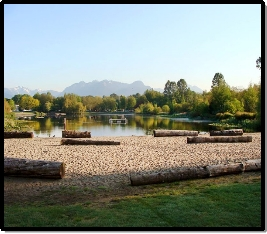
\includegraphics{tlcover.jpg}

John Hendry Park is a 27 hectare park located in the heart of East Vancouver. Frequently referred to as Trout Lake, the body of water in the centre of the park, the park itself is named after the owner of one of Vancouver’s first lumber mills, which was located in the park. 

Easily accessed from Commercial Drive, Nanaimo St, or East 12th Ave, it is a popular location for birders and nature-lovers alike in the Vancouver area. The park is also home to the Trout Lake Community Centre which provides many services to the local community. Over 135 species of birds have been observed at Trout Lake, including seven species of conservation concern. The park reaches its peak diversity during spring and fall migration, with the fewest number of birds and species during the summer. 

Certain areas of the park have proven to be better for finding different species of birds. 

Trout Lake itself usually has a large number of Mallard and wigeon, with a few other species of ducks, plus American Coots and Pied-billed Grebes from October through April. During the same time period many gulls use the lake for bathing and drinking first thing in the morning. This park has proven notable for being one of the most reliable locations for finding California and Western Gulls during this period. 

Anna’s Hummingbirds are frequently seen on the tops of small trees surrounding the lake.


\clearpage\setmargins{5mm}{19mm}{4mm}{4mm} %t,b,l,r
% pages 2, 3 and 4 are for the checklist table
% for some reason the top and bottom margins aren't
% reset with the \setmargin command above, but the 
% left and right margins are...

\linespread{0.1}
\fontfamily{phv}\fontseries{mc}\selectfont
\footnotesize
    %\tiny % usual font size
\tabcolsep=0.005cm
\rowcolors{1}{white}{Beige}
% Options: WhiteSmoke, LightCyan

%\begin{longtable}{|l|llll|llll|llll|llll|llll|llll|llll|llll|llll|llll|llll|llll|}
\begin{longtable}[c]{|p{3cm}|*{48}{c}|}
\hline
Species & \multicolumn{4}{c}{Jan} & \multicolumn{4}{c}{Feb} & \multicolumn{4}{c}{Mar} &
\multicolumn{4}{c}{Apr} & \multicolumn{4}{c}{May} & \multicolumn{4}{c}{Jun} &
\multicolumn{4}{c}{Jul} & \multicolumn{4}{c}{Aug} & \multicolumn{4}{c}{Sep} &
\multicolumn{4}{c}{Oct} & \multicolumn{4}{c}{Nov} & \multicolumn{4}{c}{Dec} \tabularnewline
\hline
\endhead
\hline
\endfoot
% latex table generated in R 3.1.0 by xtable 1.7-4 package
% Sat Apr 11 10:37:38 2015
  \hline
Greater White-fronted Goose & 
\includegraphics{bars/s-0.png} & 
\includegraphics{bars/s-0.png} & 
\includegraphics{bars/s-0.png} & 
\includegraphics{bars/s-0.png} & 
\includegraphics{bars/s-0.png} & 
\includegraphics{bars/s-0.png} & 
\includegraphics{bars/s-0.png} & 
\includegraphics{bars/s-0.png} & 
\includegraphics{bars/s-0.png} & 
\includegraphics{bars/s-0.png} & 
\includegraphics{bars/s-0.png} & 
\includegraphics{bars/s-0.png} & 
\includegraphics{bars/s-0.png} & 
\includegraphics{bars/s-0.png} & 
\includegraphics{bars/s-0.png} & 
\includegraphics{bars/s-0.png} & 
\includegraphics{bars/s-0.png} & 
\includegraphics{bars/s-0.png} & 
\includegraphics{bars/s-0.png} & 
\includegraphics{bars/s-0.png} & 
\includegraphics{bars/s-0.png} & 
\includegraphics{bars/s-0.png} & 
\includegraphics{bars/s-0.png} & 
\includegraphics{bars/s-0.png} & 
\includegraphics{bars/s-0.png} & 
\includegraphics{bars/s-0.png} & 
\includegraphics{bars/s-0.png} & 
\includegraphics{bars/s-0.png} & 
\includegraphics{bars/s-u.png} & 
\includegraphics{bars/s-0.png} & 
\includegraphics{bars/s-0.png} & 
\includegraphics{bars/s-0.png} & 
\includegraphics{bars/s-0.png} & 
\includegraphics{bars/s-0.png} & 
\includegraphics{bars/s-0.png} & 
\includegraphics{bars/s-0.png} & 
\includegraphics{bars/s-2.png} & 
\includegraphics{bars/s-2.png} & 
\includegraphics{bars/s-0.png} & 
\includegraphics{bars/s-2.png} & 
\includegraphics{bars/s-0.png} & 
\includegraphics{bars/s-0.png} & 
\includegraphics{bars/s-0.png} & 
\includegraphics{bars/s-0.png} & 
\includegraphics{bars/s-0.png} & 
\includegraphics{bars/s-0.png} & 
\includegraphics{bars/s-0.png} & 
\includegraphics{bars/s-0.png} \\ 
  Snow Goose & 
\includegraphics{bars/s-0.png} & \includegraphics{bars/s-0.png} & \includegraphics{bars/s-0.png} & \includegraphics{bars/s-0.png} & \includegraphics{bars/s-0.png} & \includegraphics{bars/s-0.png} & \includegraphics{bars/s-0.png} & \includegraphics{bars/s-0.png} & \includegraphics{bars/s-0.png} & \includegraphics{bars/s-0.png} & \includegraphics{bars/s-0.png} & \includegraphics{bars/s-0.png} & \includegraphics{bars/s-0.png} & \includegraphics{bars/s-0.png} & \includegraphics{bars/s-1.png} & \includegraphics{bars/s-3.png} & \includegraphics{bars/s-0.png} & \includegraphics{bars/s-0.png} & \includegraphics{bars/s-0.png} & \includegraphics{bars/s-0.png} & \includegraphics{bars/s-0.png} & \includegraphics{bars/s-0.png} & \includegraphics{bars/s-0.png} & \includegraphics{bars/s-0.png} & \includegraphics{bars/s-0.png} & \includegraphics{bars/s-0.png} & \includegraphics{bars/s-0.png} & \includegraphics{bars/s-0.png} & \includegraphics{bars/s-u.png} & \includegraphics{bars/s-0.png} & \includegraphics{bars/s-0.png} & \includegraphics{bars/s-0.png} & \includegraphics{bars/s-0.png} & \includegraphics{bars/s-0.png} & \includegraphics{bars/s-0.png} & \includegraphics{bars/s-0.png} & \includegraphics{bars/s-0.png} & \includegraphics{bars/s-0.png} & \includegraphics{bars/s-2.png} & \includegraphics{bars/s-0.png} & \includegraphics{bars/s-0.png} & \includegraphics{bars/s-0.png} & \includegraphics{bars/s-0.png} & \includegraphics{bars/s-0.png} & \includegraphics{bars/s-0.png} & \includegraphics{bars/s-0.png} & \includegraphics{bars/s-0.png} & \includegraphics{bars/s-0.png} \\ 
  Cackling Goose & \includegraphics{bars/s-0.png} & \includegraphics{bars/s-0.png} & \includegraphics{bars/s-0.png} & \includegraphics{bars/s-0.png} & \includegraphics{bars/s-0.png} & \includegraphics{bars/s-0.png} & \includegraphics{bars/s-0.png} & \includegraphics{bars/s-0.png} & \includegraphics{bars/s-0.png} & \includegraphics{bars/s-0.png} & \includegraphics{bars/s-0.png} & \includegraphics{bars/s-1.png} & \includegraphics{bars/s-0.png} & \includegraphics{bars/s-0.png} & \includegraphics{bars/s-0.png} & \includegraphics{bars/s-0.png} & \includegraphics{bars/s-0.png} & \includegraphics{bars/s-0.png} & \includegraphics{bars/s-2.png} & \includegraphics{bars/s-0.png} & \includegraphics{bars/s-0.png} & \includegraphics{bars/s-0.png} & \includegraphics{bars/s-0.png} & \includegraphics{bars/s-0.png} & \includegraphics{bars/s-0.png} & \includegraphics{bars/s-0.png} & \includegraphics{bars/s-0.png} & \includegraphics{bars/s-0.png} & \includegraphics{bars/s-u.png} & \includegraphics{bars/s-0.png} & \includegraphics{bars/s-0.png} & \includegraphics{bars/s-0.png} & \includegraphics{bars/s-0.png} & \includegraphics{bars/s-0.png} & \includegraphics{bars/s-0.png} & \includegraphics{bars/s-0.png} & \includegraphics{bars/s-0.png} & \includegraphics{bars/s-0.png} & \includegraphics{bars/s-0.png} & \includegraphics{bars/s-0.png} & \includegraphics{bars/s-0.png} & \includegraphics{bars/s-0.png} & \includegraphics{bars/s-0.png} & \includegraphics{bars/s-0.png} & \includegraphics{bars/s-0.png} & \includegraphics{bars/s-0.png} & \includegraphics{bars/s-0.png} & \includegraphics{bars/s-0.png} \\ 
  Canada Goose & \includegraphics{bars/s-0.png} & \includegraphics{bars/s-0.png} & \includegraphics{bars/s-0.png} & \includegraphics{bars/s-0.png} & \includegraphics{bars/s-0.png} & \includegraphics{bars/s-2.png} & \includegraphics{bars/s-2.png} & \includegraphics{bars/s-0.png} & \includegraphics{bars/s-2.png} & \includegraphics{bars/s-4.png} & \includegraphics{bars/s-3.png} & \includegraphics{bars/s-2.png} & \includegraphics{bars/s-4.png} & \includegraphics{bars/s-5.png} & \includegraphics{bars/s-1.png} & \includegraphics{bars/s-3.png} & \includegraphics{bars/s-8.png} & \includegraphics{bars/s-3.png} & \includegraphics{bars/s-2.png} & \includegraphics{bars/s-4.png} & \includegraphics{bars/s-0.png} & \includegraphics{bars/s-0.png} & \includegraphics{bars/s-2.png} & \includegraphics{bars/s-0.png} & \includegraphics{bars/s-0.png} & \includegraphics{bars/s-0.png} & \includegraphics{bars/s-0.png} & \includegraphics{bars/s-0.png} & \includegraphics{bars/s-u.png} & \includegraphics{bars/s-0.png} & \includegraphics{bars/s-0.png} & \includegraphics{bars/s-0.png} & \includegraphics{bars/s-0.png} & \includegraphics{bars/s-2.png} & \includegraphics{bars/s-3.png} & \includegraphics{bars/s-1.png} & \includegraphics{bars/s-1.png} & \includegraphics{bars/s-0.png} & \includegraphics{bars/s-2.png} & \includegraphics{bars/s-0.png} & \includegraphics{bars/s-1.png} & \includegraphics{bars/s-1.png} & \includegraphics{bars/s-0.png} & \includegraphics{bars/s-0.png} & \includegraphics{bars/s-0.png} & \includegraphics{bars/s-0.png} & \includegraphics{bars/s-0.png} & \includegraphics{bars/s-0.png} \\ 
  Trumpeter Swan & \includegraphics{bars/s-0.png} & \includegraphics{bars/s-0.png} & \includegraphics{bars/s-0.png} & \includegraphics{bars/s-0.png} & \includegraphics{bars/s-0.png} & \includegraphics{bars/s-0.png} & \includegraphics{bars/s-0.png} & \includegraphics{bars/s-0.png} & \includegraphics{bars/s-0.png} & \includegraphics{bars/s-2.png} & \includegraphics{bars/s-0.png} & \includegraphics{bars/s-0.png} & \includegraphics{bars/s-1.png} & \includegraphics{bars/s-0.png} & \includegraphics{bars/s-1.png} & \includegraphics{bars/s-0.png} & \includegraphics{bars/s-0.png} & \includegraphics{bars/s-0.png} & \includegraphics{bars/s-0.png} & \includegraphics{bars/s-0.png} & \includegraphics{bars/s-0.png} & \includegraphics{bars/s-0.png} & \includegraphics{bars/s-0.png} & \includegraphics{bars/s-0.png} & \includegraphics{bars/s-0.png} & \includegraphics{bars/s-0.png} & \includegraphics{bars/s-0.png} & \includegraphics{bars/s-0.png} & \includegraphics{bars/s-u.png} & \includegraphics{bars/s-0.png} & \includegraphics{bars/s-0.png} & \includegraphics{bars/s-0.png} & \includegraphics{bars/s-0.png} & \includegraphics{bars/s-0.png} & \includegraphics{bars/s-0.png} & \includegraphics{bars/s-0.png} & \includegraphics{bars/s-0.png} & \includegraphics{bars/s-0.png} & \includegraphics{bars/s-0.png} & \includegraphics{bars/s-2.png} & \includegraphics{bars/s-2.png} & \includegraphics{bars/s-0.png} & \includegraphics{bars/s-0.png} & \includegraphics{bars/s-0.png} & \includegraphics{bars/s-0.png} & \includegraphics{bars/s-0.png} & \includegraphics{bars/s-0.png} & \includegraphics{bars/s-0.png} \\ 
  Wood Duck & \includegraphics{bars/s-2.png} & \includegraphics{bars/s-0.png} & \includegraphics{bars/s-0.png} & \includegraphics{bars/s-0.png} & \includegraphics{bars/s-0.png} & \includegraphics{bars/s-0.png} & \includegraphics{bars/s-0.png} & \includegraphics{bars/s-0.png} & \includegraphics{bars/s-0.png} & \includegraphics{bars/s-1.png} & \includegraphics{bars/s-0.png} & \includegraphics{bars/s-0.png} & \includegraphics{bars/s-1.png} & \includegraphics{bars/s-1.png} & \includegraphics{bars/s-0.png} & \includegraphics{bars/s-0.png} & \includegraphics{bars/s-0.png} & \includegraphics{bars/s-0.png} & \includegraphics{bars/s-0.png} & \includegraphics{bars/s-1.png} & \includegraphics{bars/s-0.png} & \includegraphics{bars/s-0.png} & \includegraphics{bars/s-2.png} & \includegraphics{bars/s-0.png} & \includegraphics{bars/s-0.png} & \includegraphics{bars/s-0.png} & \includegraphics{bars/s-0.png} & \includegraphics{bars/s-0.png} & \includegraphics{bars/s-u.png} & \includegraphics{bars/s-0.png} & \includegraphics{bars/s-0.png} & \includegraphics{bars/s-0.png} & \includegraphics{bars/s-0.png} & \includegraphics{bars/s-4.png} & \includegraphics{bars/s-3.png} & \includegraphics{bars/s-0.png} & \includegraphics{bars/s-0.png} & \includegraphics{bars/s-1.png} & \includegraphics{bars/s-0.png} & \includegraphics{bars/s-0.png} & \includegraphics{bars/s-1.png} & \includegraphics{bars/s-0.png} & \includegraphics{bars/s-1.png} & \includegraphics{bars/s-0.png} & \includegraphics{bars/s-0.png} & \includegraphics{bars/s-1.png} & \includegraphics{bars/s-3.png} & \includegraphics{bars/s-0.png} \\ 
  Gadwall & \includegraphics{bars/s-0.png} & \includegraphics{bars/s-0.png} & \includegraphics{bars/s-0.png} & \includegraphics{bars/s-0.png} & \includegraphics{bars/s-0.png} & \includegraphics{bars/s-1.png} & \includegraphics{bars/s-0.png} & \includegraphics{bars/s-0.png} & \includegraphics{bars/s-0.png} & \includegraphics{bars/s-0.png} & \includegraphics{bars/s-0.png} & \includegraphics{bars/s-0.png} & \includegraphics{bars/s-0.png} & \includegraphics{bars/s-0.png} & \includegraphics{bars/s-0.png} & \includegraphics{bars/s-0.png} & \includegraphics{bars/s-0.png} & \includegraphics{bars/s-0.png} & \includegraphics{bars/s-0.png} & \includegraphics{bars/s-1.png} & \includegraphics{bars/s-0.png} & \includegraphics{bars/s-0.png} & \includegraphics{bars/s-0.png} & \includegraphics{bars/s-0.png} & \includegraphics{bars/s-0.png} & \includegraphics{bars/s-0.png} & \includegraphics{bars/s-0.png} & \includegraphics{bars/s-0.png} & \includegraphics{bars/s-u.png} & \includegraphics{bars/s-0.png} & \includegraphics{bars/s-0.png} & \includegraphics{bars/s-0.png} & \includegraphics{bars/s-0.png} & \includegraphics{bars/s-0.png} & \includegraphics{bars/s-0.png} & \includegraphics{bars/s-1.png} & \includegraphics{bars/s-0.png} & \includegraphics{bars/s-0.png} & \includegraphics{bars/s-0.png} & \includegraphics{bars/s-2.png} & \includegraphics{bars/s-2.png} & \includegraphics{bars/s-0.png} & \includegraphics{bars/s-0.png} & \includegraphics{bars/s-1.png} & \includegraphics{bars/s-0.png} & \includegraphics{bars/s-0.png} & \includegraphics{bars/s-0.png} & \includegraphics{bars/s-0.png} \\ 
  Eurasian Wigeon & \includegraphics{bars/s-6.png} & \includegraphics{bars/s-8.png} & \includegraphics{bars/s-9.png} & \includegraphics{bars/s-5.png} & \includegraphics{bars/s-7.png} & \includegraphics{bars/s-7.png} & \includegraphics{bars/s-6.png} & \includegraphics{bars/s-4.png} & \includegraphics{bars/s-5.png} & \includegraphics{bars/s-8.png} & \includegraphics{bars/s-7.png} & \includegraphics{bars/s-3.png} & \includegraphics{bars/s-2.png} & \includegraphics{bars/s-0.png} & \includegraphics{bars/s-0.png} & \includegraphics{bars/s-0.png} & \includegraphics{bars/s-0.png} & \includegraphics{bars/s-0.png} & \includegraphics{bars/s-0.png} & \includegraphics{bars/s-0.png} & \includegraphics{bars/s-0.png} & \includegraphics{bars/s-0.png} & \includegraphics{bars/s-0.png} & \includegraphics{bars/s-0.png} & \includegraphics{bars/s-0.png} & \includegraphics{bars/s-0.png} & \includegraphics{bars/s-0.png} & \includegraphics{bars/s-0.png} & \includegraphics{bars/s-u.png} & \includegraphics{bars/s-0.png} & \includegraphics{bars/s-0.png} & \includegraphics{bars/s-0.png} & \includegraphics{bars/s-0.png} & \includegraphics{bars/s-0.png} & \includegraphics{bars/s-0.png} & \includegraphics{bars/s-0.png} & \includegraphics{bars/s-0.png} & \includegraphics{bars/s-0.png} & \includegraphics{bars/s-0.png} & \includegraphics{bars/s-0.png} & \includegraphics{bars/s-1.png} & \includegraphics{bars/s-2.png} & \includegraphics{bars/s-8.png} & \includegraphics{bars/s-8.png} & \includegraphics{bars/s-5.png} & \includegraphics{bars/s-4.png} & \includegraphics{bars/s-9.png} & \includegraphics{bars/s-4.png} \\ 
  American Wigeon & \includegraphics{bars/s-9.png} & \includegraphics{bars/s-9.png} & \includegraphics{bars/s-9.png} & \includegraphics{bars/s-9.png} & \includegraphics{bars/s-9.png} & \includegraphics{bars/s-9.png} & \includegraphics{bars/s-9.png} & \includegraphics{bars/s-9.png} & \includegraphics{bars/s-9.png} & \includegraphics{bars/s-9.png} & \includegraphics{bars/s-9.png} & \includegraphics{bars/s-9.png} & \includegraphics{bars/s-9.png} & \includegraphics{bars/s-9.png} & \includegraphics{bars/s-9.png} & \includegraphics{bars/s-9.png} & \includegraphics{bars/s-5.png} & \includegraphics{bars/s-2.png} & \includegraphics{bars/s-0.png} & \includegraphics{bars/s-2.png} & \includegraphics{bars/s-0.png} & \includegraphics{bars/s-0.png} & \includegraphics{bars/s-0.png} & \includegraphics{bars/s-0.png} & \includegraphics{bars/s-0.png} & \includegraphics{bars/s-0.png} & \includegraphics{bars/s-0.png} & \includegraphics{bars/s-0.png} & \includegraphics{bars/s-u.png} & \includegraphics{bars/s-0.png} & \includegraphics{bars/s-0.png} & \includegraphics{bars/s-2.png} & \includegraphics{bars/s-0.png} & \includegraphics{bars/s-2.png} & \includegraphics{bars/s-0.png} & \includegraphics{bars/s-1.png} & \includegraphics{bars/s-2.png} & \includegraphics{bars/s-3.png} & \includegraphics{bars/s-7.png} & \includegraphics{bars/s-7.png} & \includegraphics{bars/s-9.png} & \includegraphics{bars/s-9.png} & \includegraphics{bars/s-9.png} & \includegraphics{bars/s-9.png} & \includegraphics{bars/s-9.png} & \includegraphics{bars/s-9.png} & \includegraphics{bars/s-9.png} & \includegraphics{bars/s-9.png} \\ 
  Mallard & \includegraphics{bars/s-9.png} & \includegraphics{bars/s-9.png} & \includegraphics{bars/s-9.png} & \includegraphics{bars/s-9.png} & \includegraphics{bars/s-9.png} & \includegraphics{bars/s-9.png} & \includegraphics{bars/s-9.png} & \includegraphics{bars/s-9.png} & \includegraphics{bars/s-9.png} & \includegraphics{bars/s-9.png} & \includegraphics{bars/s-9.png} & \includegraphics{bars/s-9.png} & \includegraphics{bars/s-9.png} & \includegraphics{bars/s-9.png} & \includegraphics{bars/s-9.png} & \includegraphics{bars/s-9.png} & \includegraphics{bars/s-9.png} & \includegraphics{bars/s-9.png} & \includegraphics{bars/s-9.png} & \includegraphics{bars/s-9.png} & \includegraphics{bars/s-9.png} & \includegraphics{bars/s-9.png} & \includegraphics{bars/s-9.png} & \includegraphics{bars/s-9.png} & \includegraphics{bars/s-9.png} & \includegraphics{bars/s-9.png} & \includegraphics{bars/s-9.png} & \includegraphics{bars/s-9.png} & \includegraphics{bars/s-u.png} & \includegraphics{bars/s-9.png} & \includegraphics{bars/s-9.png} & \includegraphics{bars/s-9.png} & \includegraphics{bars/s-9.png} & \includegraphics{bars/s-9.png} & \includegraphics{bars/s-9.png} & \includegraphics{bars/s-9.png} & \includegraphics{bars/s-9.png} & \includegraphics{bars/s-9.png} & \includegraphics{bars/s-9.png} & \includegraphics{bars/s-9.png} & \includegraphics{bars/s-9.png} & \includegraphics{bars/s-9.png} & \includegraphics{bars/s-9.png} & \includegraphics{bars/s-9.png} & \includegraphics{bars/s-9.png} & \includegraphics{bars/s-9.png} & \includegraphics{bars/s-9.png} & \includegraphics{bars/s-9.png} \\ 
  Northern Shoveler & \includegraphics{bars/s-9.png} & \includegraphics{bars/s-9.png} & \includegraphics{bars/s-9.png} & \includegraphics{bars/s-9.png} & \includegraphics{bars/s-9.png} & \includegraphics{bars/s-9.png} & \includegraphics{bars/s-9.png} & \includegraphics{bars/s-9.png} & \includegraphics{bars/s-9.png} & \includegraphics{bars/s-9.png} & \includegraphics{bars/s-9.png} & \includegraphics{bars/s-8.png} & \includegraphics{bars/s-8.png} & \includegraphics{bars/s-6.png} & \includegraphics{bars/s-6.png} & \includegraphics{bars/s-8.png} & \includegraphics{bars/s-3.png} & \includegraphics{bars/s-3.png} & \includegraphics{bars/s-0.png} & \includegraphics{bars/s-0.png} & \includegraphics{bars/s-0.png} & \includegraphics{bars/s-0.png} & \includegraphics{bars/s-0.png} & \includegraphics{bars/s-0.png} & \includegraphics{bars/s-0.png} & \includegraphics{bars/s-0.png} & \includegraphics{bars/s-0.png} & \includegraphics{bars/s-0.png} & \includegraphics{bars/s-u.png} & \includegraphics{bars/s-0.png} & \includegraphics{bars/s-0.png} & \includegraphics{bars/s-0.png} & \includegraphics{bars/s-2.png} & \includegraphics{bars/s-0.png} & \includegraphics{bars/s-0.png} & \includegraphics{bars/s-2.png} & \includegraphics{bars/s-2.png} & \includegraphics{bars/s-2.png} & \includegraphics{bars/s-2.png} & \includegraphics{bars/s-2.png} & \includegraphics{bars/s-8.png} & \includegraphics{bars/s-7.png} & \includegraphics{bars/s-9.png} & \includegraphics{bars/s-9.png} & \includegraphics{bars/s-9.png} & \includegraphics{bars/s-8.png} & \includegraphics{bars/s-9.png} & \includegraphics{bars/s-7.png} \\ 
  Northern Pintail & \includegraphics{bars/s-0.png} & \includegraphics{bars/s-0.png} & \includegraphics{bars/s-0.png} & \includegraphics{bars/s-0.png} & \includegraphics{bars/s-0.png} & \includegraphics{bars/s-1.png} & \includegraphics{bars/s-0.png} & \includegraphics{bars/s-0.png} & \includegraphics{bars/s-0.png} & \includegraphics{bars/s-0.png} & \includegraphics{bars/s-0.png} & \includegraphics{bars/s-1.png} & \includegraphics{bars/s-0.png} & \includegraphics{bars/s-0.png} & \includegraphics{bars/s-0.png} & \includegraphics{bars/s-0.png} & \includegraphics{bars/s-0.png} & \includegraphics{bars/s-0.png} & \includegraphics{bars/s-0.png} & \includegraphics{bars/s-0.png} & \includegraphics{bars/s-0.png} & \includegraphics{bars/s-0.png} & \includegraphics{bars/s-0.png} & \includegraphics{bars/s-0.png} & \includegraphics{bars/s-0.png} & \includegraphics{bars/s-0.png} & \includegraphics{bars/s-0.png} & \includegraphics{bars/s-0.png} & \includegraphics{bars/s-u.png} & \includegraphics{bars/s-0.png} & \includegraphics{bars/s-0.png} & \includegraphics{bars/s-4.png} & \includegraphics{bars/s-2.png} & \includegraphics{bars/s-0.png} & \includegraphics{bars/s-0.png} & \includegraphics{bars/s-0.png} & \includegraphics{bars/s-0.png} & \includegraphics{bars/s-0.png} & \includegraphics{bars/s-0.png} & \includegraphics{bars/s-0.png} & \includegraphics{bars/s-0.png} & \includegraphics{bars/s-1.png} & \includegraphics{bars/s-0.png} & \includegraphics{bars/s-0.png} & \includegraphics{bars/s-0.png} & \includegraphics{bars/s-0.png} & \includegraphics{bars/s-0.png} & \includegraphics{bars/s-0.png} \\ 
  Green-winged Teal & \includegraphics{bars/s-0.png} & \includegraphics{bars/s-0.png} & \includegraphics{bars/s-0.png} & \includegraphics{bars/s-1.png} & \includegraphics{bars/s-0.png} & \includegraphics{bars/s-2.png} & \includegraphics{bars/s-1.png} & \includegraphics{bars/s-0.png} & \includegraphics{bars/s-0.png} & \includegraphics{bars/s-0.png} & \includegraphics{bars/s-0.png} & \includegraphics{bars/s-0.png} & \includegraphics{bars/s-0.png} & \includegraphics{bars/s-0.png} & \includegraphics{bars/s-0.png} & \includegraphics{bars/s-0.png} & \includegraphics{bars/s-0.png} & \includegraphics{bars/s-0.png} & \includegraphics{bars/s-0.png} & \includegraphics{bars/s-0.png} & \includegraphics{bars/s-0.png} & \includegraphics{bars/s-0.png} & \includegraphics{bars/s-0.png} & \includegraphics{bars/s-0.png} & \includegraphics{bars/s-0.png} & \includegraphics{bars/s-0.png} & \includegraphics{bars/s-0.png} & \includegraphics{bars/s-0.png} & \includegraphics{bars/s-u.png} & \includegraphics{bars/s-0.png} & \includegraphics{bars/s-0.png} & \includegraphics{bars/s-2.png} & \includegraphics{bars/s-2.png} & \includegraphics{bars/s-2.png} & \includegraphics{bars/s-3.png} & \includegraphics{bars/s-2.png} & \includegraphics{bars/s-1.png} & \includegraphics{bars/s-2.png} & \includegraphics{bars/s-2.png} & \includegraphics{bars/s-3.png} & \includegraphics{bars/s-1.png} & \includegraphics{bars/s-1.png} & \includegraphics{bars/s-0.png} & \includegraphics{bars/s-1.png} & \includegraphics{bars/s-0.png} & \includegraphics{bars/s-0.png} & \includegraphics{bars/s-0.png} & \includegraphics{bars/s-0.png} \\ 
  Ring-necked Duck & \includegraphics{bars/s-2.png} & \includegraphics{bars/s-4.png} & \includegraphics{bars/s-5.png} & \includegraphics{bars/s-7.png} & \includegraphics{bars/s-3.png} & \includegraphics{bars/s-4.png} & \includegraphics{bars/s-4.png} & \includegraphics{bars/s-7.png} & \includegraphics{bars/s-4.png} & \includegraphics{bars/s-2.png} & \includegraphics{bars/s-2.png} & \includegraphics{bars/s-4.png} & \includegraphics{bars/s-0.png} & \includegraphics{bars/s-5.png} & \includegraphics{bars/s-4.png} & \includegraphics{bars/s-2.png} & \includegraphics{bars/s-5.png} & \includegraphics{bars/s-3.png} & \includegraphics{bars/s-3.png} & \includegraphics{bars/s-0.png} & \includegraphics{bars/s-0.png} & \includegraphics{bars/s-0.png} & \includegraphics{bars/s-0.png} & \includegraphics{bars/s-0.png} & \includegraphics{bars/s-0.png} & \includegraphics{bars/s-0.png} & \includegraphics{bars/s-0.png} & \includegraphics{bars/s-0.png} & \includegraphics{bars/s-u.png} & \includegraphics{bars/s-0.png} & \includegraphics{bars/s-0.png} & \includegraphics{bars/s-0.png} & \includegraphics{bars/s-0.png} & \includegraphics{bars/s-0.png} & \includegraphics{bars/s-0.png} & \includegraphics{bars/s-0.png} & \includegraphics{bars/s-3.png} & \includegraphics{bars/s-2.png} & \includegraphics{bars/s-2.png} & \includegraphics{bars/s-2.png} & \includegraphics{bars/s-4.png} & \includegraphics{bars/s-6.png} & \includegraphics{bars/s-8.png} & \includegraphics{bars/s-7.png} & \includegraphics{bars/s-2.png} & \includegraphics{bars/s-5.png} & \includegraphics{bars/s-9.png} & \includegraphics{bars/s-4.png} \\ 
  Lesser Scaup & \includegraphics{bars/s-3.png} & \includegraphics{bars/s-2.png} & \includegraphics{bars/s-4.png} & \includegraphics{bars/s-3.png} & \includegraphics{bars/s-2.png} & \includegraphics{bars/s-4.png} & \includegraphics{bars/s-4.png} & \includegraphics{bars/s-6.png} & \includegraphics{bars/s-5.png} & \includegraphics{bars/s-5.png} & \includegraphics{bars/s-6.png} & \includegraphics{bars/s-4.png} & \includegraphics{bars/s-5.png} & \includegraphics{bars/s-6.png} & \includegraphics{bars/s-5.png} & \includegraphics{bars/s-6.png} & \includegraphics{bars/s-0.png} & \includegraphics{bars/s-2.png} & \includegraphics{bars/s-0.png} & \includegraphics{bars/s-0.png} & \includegraphics{bars/s-0.png} & \includegraphics{bars/s-0.png} & \includegraphics{bars/s-0.png} & \includegraphics{bars/s-0.png} & \includegraphics{bars/s-0.png} & \includegraphics{bars/s-0.png} & \includegraphics{bars/s-0.png} & \includegraphics{bars/s-0.png} & \includegraphics{bars/s-u.png} & \includegraphics{bars/s-0.png} & \includegraphics{bars/s-0.png} & \includegraphics{bars/s-0.png} & \includegraphics{bars/s-0.png} & \includegraphics{bars/s-0.png} & \includegraphics{bars/s-0.png} & \includegraphics{bars/s-0.png} & \includegraphics{bars/s-0.png} & \includegraphics{bars/s-0.png} & \includegraphics{bars/s-0.png} & \includegraphics{bars/s-0.png} & \includegraphics{bars/s-0.png} & \includegraphics{bars/s-0.png} & \includegraphics{bars/s-1.png} & \includegraphics{bars/s-0.png} & \includegraphics{bars/s-0.png} & \includegraphics{bars/s-0.png} & \includegraphics{bars/s-0.png} & \includegraphics{bars/s-0.png} \\ 
  Bufflehead & \includegraphics{bars/s-3.png} & \includegraphics{bars/s-4.png} & \includegraphics{bars/s-4.png} & \includegraphics{bars/s-4.png} & \includegraphics{bars/s-4.png} & \includegraphics{bars/s-7.png} & \includegraphics{bars/s-4.png} & \includegraphics{bars/s-5.png} & \includegraphics{bars/s-2.png} & \includegraphics{bars/s-5.png} & \includegraphics{bars/s-8.png} & \includegraphics{bars/s-7.png} & \includegraphics{bars/s-6.png} & \includegraphics{bars/s-6.png} & \includegraphics{bars/s-8.png} & \includegraphics{bars/s-7.png} & \includegraphics{bars/s-0.png} & \includegraphics{bars/s-2.png} & \includegraphics{bars/s-0.png} & \includegraphics{bars/s-2.png} & \includegraphics{bars/s-0.png} & \includegraphics{bars/s-0.png} & \includegraphics{bars/s-0.png} & \includegraphics{bars/s-0.png} & \includegraphics{bars/s-0.png} & \includegraphics{bars/s-0.png} & \includegraphics{bars/s-0.png} & \includegraphics{bars/s-0.png} & \includegraphics{bars/s-u.png} & \includegraphics{bars/s-0.png} & \includegraphics{bars/s-0.png} & \includegraphics{bars/s-0.png} & \includegraphics{bars/s-0.png} & \includegraphics{bars/s-0.png} & \includegraphics{bars/s-0.png} & \includegraphics{bars/s-0.png} & \includegraphics{bars/s-0.png} & \includegraphics{bars/s-1.png} & \includegraphics{bars/s-2.png} & \includegraphics{bars/s-2.png} & \includegraphics{bars/s-4.png} & \includegraphics{bars/s-4.png} & \includegraphics{bars/s-3.png} & \includegraphics{bars/s-7.png} & \includegraphics{bars/s-5.png} & \includegraphics{bars/s-3.png} & \includegraphics{bars/s-3.png} & \includegraphics{bars/s-7.png} \\ 
  Common Goldeneye & \includegraphics{bars/s-0.png} & \includegraphics{bars/s-0.png} & \includegraphics{bars/s-0.png} & \includegraphics{bars/s-0.png} & \includegraphics{bars/s-1.png} & \includegraphics{bars/s-0.png} & \includegraphics{bars/s-0.png} & \includegraphics{bars/s-0.png} & \includegraphics{bars/s-0.png} & \includegraphics{bars/s-1.png} & \includegraphics{bars/s-0.png} & \includegraphics{bars/s-0.png} & \includegraphics{bars/s-0.png} & \includegraphics{bars/s-0.png} & \includegraphics{bars/s-0.png} & \includegraphics{bars/s-0.png} & \includegraphics{bars/s-0.png} & \includegraphics{bars/s-0.png} & \includegraphics{bars/s-0.png} & \includegraphics{bars/s-0.png} & \includegraphics{bars/s-0.png} & \includegraphics{bars/s-0.png} & \includegraphics{bars/s-0.png} & \includegraphics{bars/s-0.png} & \includegraphics{bars/s-0.png} & \includegraphics{bars/s-0.png} & \includegraphics{bars/s-0.png} & \includegraphics{bars/s-0.png} & \includegraphics{bars/s-u.png} & \includegraphics{bars/s-0.png} & \includegraphics{bars/s-0.png} & \includegraphics{bars/s-0.png} & \includegraphics{bars/s-0.png} & \includegraphics{bars/s-0.png} & \includegraphics{bars/s-0.png} & \includegraphics{bars/s-0.png} & \includegraphics{bars/s-0.png} & \includegraphics{bars/s-0.png} & \includegraphics{bars/s-0.png} & \includegraphics{bars/s-0.png} & \includegraphics{bars/s-1.png} & \includegraphics{bars/s-0.png} & \includegraphics{bars/s-0.png} & \includegraphics{bars/s-0.png} & \includegraphics{bars/s-0.png} & \includegraphics{bars/s-1.png} & \includegraphics{bars/s-0.png} & \includegraphics{bars/s-0.png} \\ 
  Hooded Merganser & \includegraphics{bars/s-6.png} & \includegraphics{bars/s-5.png} & \includegraphics{bars/s-3.png} & \includegraphics{bars/s-7.png} & \includegraphics{bars/s-4.png} & \includegraphics{bars/s-5.png} & \includegraphics{bars/s-3.png} & \includegraphics{bars/s-7.png} & \includegraphics{bars/s-5.png} & \includegraphics{bars/s-4.png} & \includegraphics{bars/s-1.png} & \includegraphics{bars/s-1.png} & \includegraphics{bars/s-1.png} & \includegraphics{bars/s-1.png} & \includegraphics{bars/s-0.png} & \includegraphics{bars/s-2.png} & \includegraphics{bars/s-0.png} & \includegraphics{bars/s-2.png} & \includegraphics{bars/s-0.png} & \includegraphics{bars/s-0.png} & \includegraphics{bars/s-0.png} & \includegraphics{bars/s-0.png} & \includegraphics{bars/s-2.png} & \includegraphics{bars/s-0.png} & \includegraphics{bars/s-0.png} & \includegraphics{bars/s-0.png} & \includegraphics{bars/s-3.png} & \includegraphics{bars/s-3.png} & \includegraphics{bars/s-u.png} & \includegraphics{bars/s-0.png} & \includegraphics{bars/s-0.png} & \includegraphics{bars/s-0.png} & \includegraphics{bars/s-0.png} & \includegraphics{bars/s-0.png} & \includegraphics{bars/s-0.png} & \includegraphics{bars/s-0.png} & \includegraphics{bars/s-0.png} & \includegraphics{bars/s-0.png} & \includegraphics{bars/s-0.png} & \includegraphics{bars/s-0.png} & \includegraphics{bars/s-4.png} & \includegraphics{bars/s-4.png} & \includegraphics{bars/s-7.png} & \includegraphics{bars/s-6.png} & \includegraphics{bars/s-5.png} & \includegraphics{bars/s-4.png} & \includegraphics{bars/s-5.png} & \includegraphics{bars/s-4.png} \\ 
  Common Merganser & \includegraphics{bars/s-9.png} & \includegraphics{bars/s-8.png} & \includegraphics{bars/s-9.png} & \includegraphics{bars/s-9.png} & \includegraphics{bars/s-6.png} & \includegraphics{bars/s-8.png} & \includegraphics{bars/s-6.png} & \includegraphics{bars/s-3.png} & \includegraphics{bars/s-2.png} & \includegraphics{bars/s-2.png} & \includegraphics{bars/s-0.png} & \includegraphics{bars/s-2.png} & \includegraphics{bars/s-1.png} & \includegraphics{bars/s-0.png} & \includegraphics{bars/s-0.png} & \includegraphics{bars/s-1.png} & \includegraphics{bars/s-0.png} & \includegraphics{bars/s-0.png} & \includegraphics{bars/s-0.png} & \includegraphics{bars/s-0.png} & \includegraphics{bars/s-0.png} & \includegraphics{bars/s-0.png} & \includegraphics{bars/s-0.png} & \includegraphics{bars/s-0.png} & \includegraphics{bars/s-0.png} & \includegraphics{bars/s-0.png} & \includegraphics{bars/s-0.png} & \includegraphics{bars/s-0.png} & \includegraphics{bars/s-u.png} & \includegraphics{bars/s-0.png} & \includegraphics{bars/s-0.png} & \includegraphics{bars/s-0.png} & \includegraphics{bars/s-0.png} & \includegraphics{bars/s-0.png} & \includegraphics{bars/s-0.png} & \includegraphics{bars/s-0.png} & \includegraphics{bars/s-0.png} & \includegraphics{bars/s-0.png} & \includegraphics{bars/s-0.png} & \includegraphics{bars/s-0.png} & \includegraphics{bars/s-2.png} & \includegraphics{bars/s-5.png} & \includegraphics{bars/s-5.png} & \includegraphics{bars/s-9.png} & \includegraphics{bars/s-4.png} & \includegraphics{bars/s-2.png} & \includegraphics{bars/s-8.png} & \includegraphics{bars/s-4.png} \\ 
  Ruddy Duck & \includegraphics{bars/s-0.png} & \includegraphics{bars/s-0.png} & \includegraphics{bars/s-0.png} & \includegraphics{bars/s-0.png} & \includegraphics{bars/s-0.png} & \includegraphics{bars/s-0.png} & \includegraphics{bars/s-0.png} & \includegraphics{bars/s-0.png} & \includegraphics{bars/s-0.png} & \includegraphics{bars/s-3.png} & \includegraphics{bars/s-0.png} & \includegraphics{bars/s-0.png} & \includegraphics{bars/s-1.png} & \includegraphics{bars/s-1.png} & \includegraphics{bars/s-0.png} & \includegraphics{bars/s-0.png} & \includegraphics{bars/s-0.png} & \includegraphics{bars/s-0.png} & \includegraphics{bars/s-0.png} & \includegraphics{bars/s-0.png} & \includegraphics{bars/s-0.png} & \includegraphics{bars/s-0.png} & \includegraphics{bars/s-0.png} & \includegraphics{bars/s-0.png} & \includegraphics{bars/s-0.png} & \includegraphics{bars/s-0.png} & \includegraphics{bars/s-0.png} & \includegraphics{bars/s-0.png} & \includegraphics{bars/s-u.png} & \includegraphics{bars/s-0.png} & \includegraphics{bars/s-0.png} & \includegraphics{bars/s-0.png} & \includegraphics{bars/s-0.png} & \includegraphics{bars/s-0.png} & \includegraphics{bars/s-0.png} & \includegraphics{bars/s-0.png} & \includegraphics{bars/s-0.png} & \includegraphics{bars/s-0.png} & \includegraphics{bars/s-0.png} & \includegraphics{bars/s-0.png} & \includegraphics{bars/s-0.png} & \includegraphics{bars/s-0.png} & \includegraphics{bars/s-0.png} & \includegraphics{bars/s-0.png} & \includegraphics{bars/s-0.png} & \includegraphics{bars/s-0.png} & \includegraphics{bars/s-0.png} & \includegraphics{bars/s-0.png} \\ 
  Pied-billed Grebe & \includegraphics{bars/s-9.png} & \includegraphics{bars/s-7.png} & \includegraphics{bars/s-8.png} & \includegraphics{bars/s-7.png} & \includegraphics{bars/s-7.png} & \includegraphics{bars/s-8.png} & \includegraphics{bars/s-8.png} & \includegraphics{bars/s-8.png} & \includegraphics{bars/s-6.png} & \includegraphics{bars/s-9.png} & \includegraphics{bars/s-9.png} & \includegraphics{bars/s-6.png} & \includegraphics{bars/s-8.png} & \includegraphics{bars/s-6.png} & \includegraphics{bars/s-5.png} & \includegraphics{bars/s-4.png} & \includegraphics{bars/s-5.png} & \includegraphics{bars/s-6.png} & \includegraphics{bars/s-2.png} & \includegraphics{bars/s-2.png} & \includegraphics{bars/s-0.png} & \includegraphics{bars/s-0.png} & \includegraphics{bars/s-0.png} & \includegraphics{bars/s-0.png} & \includegraphics{bars/s-0.png} & \includegraphics{bars/s-0.png} & \includegraphics{bars/s-3.png} & \includegraphics{bars/s-0.png} & \includegraphics{bars/s-u.png} & \includegraphics{bars/s-0.png} & \includegraphics{bars/s-0.png} & \includegraphics{bars/s-4.png} & \includegraphics{bars/s-8.png} & \includegraphics{bars/s-9.png} & \includegraphics{bars/s-9.png} & \includegraphics{bars/s-9.png} & \includegraphics{bars/s-9.png} & \includegraphics{bars/s-9.png} & \includegraphics{bars/s-9.png} & \includegraphics{bars/s-9.png} & \includegraphics{bars/s-9.png} & \includegraphics{bars/s-9.png} & \includegraphics{bars/s-9.png} & \includegraphics{bars/s-8.png} & \includegraphics{bars/s-4.png} & \includegraphics{bars/s-5.png} & \includegraphics{bars/s-8.png} & \includegraphics{bars/s-7.png} \\ 
  Double-crested Cormorant & \includegraphics{bars/s-4.png} & \includegraphics{bars/s-4.png} & \includegraphics{bars/s-7.png} & \includegraphics{bars/s-7.png} & \includegraphics{bars/s-5.png} & \includegraphics{bars/s-8.png} & \includegraphics{bars/s-7.png} & \includegraphics{bars/s-7.png} & \includegraphics{bars/s-9.png} & \includegraphics{bars/s-8.png} & \includegraphics{bars/s-5.png} & \includegraphics{bars/s-8.png} & \includegraphics{bars/s-6.png} & \includegraphics{bars/s-7.png} & \includegraphics{bars/s-5.png} & \includegraphics{bars/s-2.png} & \includegraphics{bars/s-3.png} & \includegraphics{bars/s-5.png} & \includegraphics{bars/s-3.png} & \includegraphics{bars/s-4.png} & \includegraphics{bars/s-5.png} & \includegraphics{bars/s-5.png} & \includegraphics{bars/s-4.png} & \includegraphics{bars/s-4.png} & \includegraphics{bars/s-7.png} & \includegraphics{bars/s-0.png} & \includegraphics{bars/s-3.png} & \includegraphics{bars/s-0.png} & \includegraphics{bars/s-u.png} & \includegraphics{bars/s-4.png} & \includegraphics{bars/s-0.png} & \includegraphics{bars/s-2.png} & \includegraphics{bars/s-3.png} & \includegraphics{bars/s-0.png} & \includegraphics{bars/s-3.png} & \includegraphics{bars/s-2.png} & \includegraphics{bars/s-0.png} & \includegraphics{bars/s-2.png} & \includegraphics{bars/s-3.png} & \includegraphics{bars/s-3.png} & \includegraphics{bars/s-2.png} & \includegraphics{bars/s-4.png} & \includegraphics{bars/s-4.png} & \includegraphics{bars/s-4.png} & \includegraphics{bars/s-0.png} & \includegraphics{bars/s-0.png} & \includegraphics{bars/s-3.png} & \includegraphics{bars/s-4.png} \\ 
  Great Blue Heron & \includegraphics{bars/s-2.png} & \includegraphics{bars/s-3.png} & \includegraphics{bars/s-4.png} & \includegraphics{bars/s-2.png} & \includegraphics{bars/s-4.png} & \includegraphics{bars/s-5.png} & \includegraphics{bars/s-1.png} & \includegraphics{bars/s-3.png} & \includegraphics{bars/s-1.png} & \includegraphics{bars/s-2.png} & \includegraphics{bars/s-4.png} & \includegraphics{bars/s-6.png} & \includegraphics{bars/s-3.png} & \includegraphics{bars/s-2.png} & \includegraphics{bars/s-2.png} & \includegraphics{bars/s-4.png} & \includegraphics{bars/s-5.png} & \includegraphics{bars/s-9.png} & \includegraphics{bars/s-2.png} & \includegraphics{bars/s-3.png} & \includegraphics{bars/s-5.png} & \includegraphics{bars/s-0.png} & \includegraphics{bars/s-2.png} & \includegraphics{bars/s-0.png} & \includegraphics{bars/s-0.png} & \includegraphics{bars/s-0.png} & \includegraphics{bars/s-0.png} & \includegraphics{bars/s-0.png} & \includegraphics{bars/s-u.png} & \includegraphics{bars/s-2.png} & \includegraphics{bars/s-0.png} & \includegraphics{bars/s-0.png} & \includegraphics{bars/s-0.png} & \includegraphics{bars/s-0.png} & \includegraphics{bars/s-0.png} & \includegraphics{bars/s-1.png} & \includegraphics{bars/s-1.png} & \includegraphics{bars/s-0.png} & \includegraphics{bars/s-3.png} & \includegraphics{bars/s-5.png} & \includegraphics{bars/s-1.png} & \includegraphics{bars/s-3.png} & \includegraphics{bars/s-1.png} & \includegraphics{bars/s-4.png} & \includegraphics{bars/s-3.png} & \includegraphics{bars/s-1.png} & \includegraphics{bars/s-5.png} & \includegraphics{bars/s-4.png} \\ 
  Turkey Vulture & \includegraphics{bars/s-0.png} & \includegraphics{bars/s-0.png} & \includegraphics{bars/s-0.png} & \includegraphics{bars/s-0.png} & \includegraphics{bars/s-0.png} & \includegraphics{bars/s-0.png} & \includegraphics{bars/s-0.png} & \includegraphics{bars/s-0.png} & \includegraphics{bars/s-0.png} & \includegraphics{bars/s-1.png} & \includegraphics{bars/s-0.png} & \includegraphics{bars/s-0.png} & \includegraphics{bars/s-0.png} & \includegraphics{bars/s-0.png} & \includegraphics{bars/s-1.png} & \includegraphics{bars/s-0.png} & \includegraphics{bars/s-0.png} & \includegraphics{bars/s-0.png} & \includegraphics{bars/s-0.png} & \includegraphics{bars/s-0.png} & \includegraphics{bars/s-0.png} & \includegraphics{bars/s-0.png} & \includegraphics{bars/s-0.png} & \includegraphics{bars/s-0.png} & \includegraphics{bars/s-0.png} & \includegraphics{bars/s-0.png} & \includegraphics{bars/s-0.png} & \includegraphics{bars/s-0.png} & \includegraphics{bars/s-u.png} & \includegraphics{bars/s-0.png} & \includegraphics{bars/s-0.png} & \includegraphics{bars/s-0.png} & \includegraphics{bars/s-0.png} & \includegraphics{bars/s-0.png} & \includegraphics{bars/s-0.png} & \includegraphics{bars/s-0.png} & \includegraphics{bars/s-1.png} & \includegraphics{bars/s-0.png} & \includegraphics{bars/s-0.png} & \includegraphics{bars/s-0.png} & \includegraphics{bars/s-0.png} & \includegraphics{bars/s-0.png} & \includegraphics{bars/s-0.png} & \includegraphics{bars/s-0.png} & \includegraphics{bars/s-0.png} & \includegraphics{bars/s-0.png} & \includegraphics{bars/s-0.png} & \includegraphics{bars/s-0.png} \\ 
  Osprey & \includegraphics{bars/s-0.png} & \includegraphics{bars/s-0.png} & \includegraphics{bars/s-0.png} & \includegraphics{bars/s-0.png} & \includegraphics{bars/s-0.png} & \includegraphics{bars/s-0.png} & \includegraphics{bars/s-0.png} & \includegraphics{bars/s-0.png} & \includegraphics{bars/s-0.png} & \includegraphics{bars/s-0.png} & \includegraphics{bars/s-0.png} & \includegraphics{bars/s-0.png} & \includegraphics{bars/s-0.png} & \includegraphics{bars/s-0.png} & \includegraphics{bars/s-1.png} & \includegraphics{bars/s-0.png} & \includegraphics{bars/s-0.png} & \includegraphics{bars/s-2.png} & \includegraphics{bars/s-0.png} & \includegraphics{bars/s-1.png} & \includegraphics{bars/s-0.png} & \includegraphics{bars/s-0.png} & \includegraphics{bars/s-2.png} & \includegraphics{bars/s-0.png} & \includegraphics{bars/s-0.png} & \includegraphics{bars/s-0.png} & \includegraphics{bars/s-0.png} & \includegraphics{bars/s-0.png} & \includegraphics{bars/s-u.png} & \includegraphics{bars/s-0.png} & \includegraphics{bars/s-0.png} & \includegraphics{bars/s-0.png} & \includegraphics{bars/s-2.png} & \includegraphics{bars/s-0.png} & \includegraphics{bars/s-2.png} & \includegraphics{bars/s-0.png} & \includegraphics{bars/s-0.png} & \includegraphics{bars/s-0.png} & \includegraphics{bars/s-0.png} & \includegraphics{bars/s-0.png} & \includegraphics{bars/s-0.png} & \includegraphics{bars/s-0.png} & \includegraphics{bars/s-0.png} & \includegraphics{bars/s-0.png} & \includegraphics{bars/s-0.png} & \includegraphics{bars/s-0.png} & \includegraphics{bars/s-0.png} & \includegraphics{bars/s-0.png} \\ 
  Sharp-shinned Hawk & \includegraphics{bars/s-0.png} & \includegraphics{bars/s-0.png} & \includegraphics{bars/s-0.png} & \includegraphics{bars/s-1.png} & \includegraphics{bars/s-0.png} & \includegraphics{bars/s-1.png} & \includegraphics{bars/s-0.png} & \includegraphics{bars/s-0.png} & \includegraphics{bars/s-1.png} & \includegraphics{bars/s-0.png} & \includegraphics{bars/s-0.png} & \includegraphics{bars/s-1.png} & \includegraphics{bars/s-0.png} & \includegraphics{bars/s-0.png} & \includegraphics{bars/s-0.png} & \includegraphics{bars/s-0.png} & \includegraphics{bars/s-0.png} & \includegraphics{bars/s-0.png} & \includegraphics{bars/s-2.png} & \includegraphics{bars/s-0.png} & \includegraphics{bars/s-0.png} & \includegraphics{bars/s-0.png} & \includegraphics{bars/s-0.png} & \includegraphics{bars/s-0.png} & \includegraphics{bars/s-0.png} & \includegraphics{bars/s-0.png} & \includegraphics{bars/s-0.png} & \includegraphics{bars/s-0.png} & \includegraphics{bars/s-u.png} & \includegraphics{bars/s-0.png} & \includegraphics{bars/s-0.png} & \includegraphics{bars/s-0.png} & \includegraphics{bars/s-2.png} & \includegraphics{bars/s-0.png} & \includegraphics{bars/s-0.png} & \includegraphics{bars/s-0.png} & \includegraphics{bars/s-1.png} & \includegraphics{bars/s-1.png} & \includegraphics{bars/s-0.png} & \includegraphics{bars/s-0.png} & \includegraphics{bars/s-0.png} & \includegraphics{bars/s-0.png} & \includegraphics{bars/s-0.png} & \includegraphics{bars/s-0.png} & \includegraphics{bars/s-0.png} & \includegraphics{bars/s-0.png} & \includegraphics{bars/s-0.png} & \includegraphics{bars/s-0.png} \\ 
  Cooper's Hawk & \includegraphics{bars/s-0.png} & \includegraphics{bars/s-1.png} & \includegraphics{bars/s-0.png} & \includegraphics{bars/s-1.png} & \includegraphics{bars/s-0.png} & \includegraphics{bars/s-1.png} & \includegraphics{bars/s-1.png} & \includegraphics{bars/s-0.png} & \includegraphics{bars/s-0.png} & \includegraphics{bars/s-0.png} & \includegraphics{bars/s-0.png} & \includegraphics{bars/s-3.png} & \includegraphics{bars/s-2.png} & \includegraphics{bars/s-1.png} & \includegraphics{bars/s-1.png} & \includegraphics{bars/s-1.png} & \includegraphics{bars/s-3.png} & \includegraphics{bars/s-0.png} & \includegraphics{bars/s-0.png} & \includegraphics{bars/s-1.png} & \includegraphics{bars/s-0.png} & \includegraphics{bars/s-0.png} & \includegraphics{bars/s-0.png} & \includegraphics{bars/s-0.png} & \includegraphics{bars/s-0.png} & \includegraphics{bars/s-0.png} & \includegraphics{bars/s-0.png} & \includegraphics{bars/s-0.png} & \includegraphics{bars/s-u.png} & \includegraphics{bars/s-0.png} & \includegraphics{bars/s-4.png} & \includegraphics{bars/s-0.png} & \includegraphics{bars/s-2.png} & \includegraphics{bars/s-5.png} & \includegraphics{bars/s-5.png} & \includegraphics{bars/s-2.png} & \includegraphics{bars/s-2.png} & \includegraphics{bars/s-0.png} & \includegraphics{bars/s-3.png} & \includegraphics{bars/s-2.png} & \includegraphics{bars/s-1.png} & \includegraphics{bars/s-0.png} & \includegraphics{bars/s-0.png} & \includegraphics{bars/s-0.png} & \includegraphics{bars/s-2.png} & \includegraphics{bars/s-0.png} & \includegraphics{bars/s-5.png} & \includegraphics{bars/s-0.png} \\ 
  Bald Eagle & \includegraphics{bars/s-4.png} & \includegraphics{bars/s-3.png} & \includegraphics{bars/s-4.png} & \includegraphics{bars/s-3.png} & \includegraphics{bars/s-4.png} & \includegraphics{bars/s-5.png} & \includegraphics{bars/s-3.png} & \includegraphics{bars/s-5.png} & \includegraphics{bars/s-3.png} & \includegraphics{bars/s-2.png} & \includegraphics{bars/s-2.png} & \includegraphics{bars/s-5.png} & \includegraphics{bars/s-1.png} & \includegraphics{bars/s-0.png} & \includegraphics{bars/s-2.png} & \includegraphics{bars/s-0.png} & \includegraphics{bars/s-0.png} & \includegraphics{bars/s-3.png} & \includegraphics{bars/s-3.png} & \includegraphics{bars/s-2.png} & \includegraphics{bars/s-5.png} & \includegraphics{bars/s-0.png} & \includegraphics{bars/s-2.png} & \includegraphics{bars/s-0.png} & \includegraphics{bars/s-0.png} & \includegraphics{bars/s-0.png} & \includegraphics{bars/s-3.png} & \includegraphics{bars/s-0.png} & \includegraphics{bars/s-u.png} & \includegraphics{bars/s-0.png} & \includegraphics{bars/s-0.png} & \includegraphics{bars/s-0.png} & \includegraphics{bars/s-0.png} & \includegraphics{bars/s-0.png} & \includegraphics{bars/s-0.png} & \includegraphics{bars/s-0.png} & \includegraphics{bars/s-2.png} & \includegraphics{bars/s-0.png} & \includegraphics{bars/s-2.png} & \includegraphics{bars/s-2.png} & \includegraphics{bars/s-1.png} & \includegraphics{bars/s-1.png} & \includegraphics{bars/s-0.png} & \includegraphics{bars/s-2.png} & \includegraphics{bars/s-4.png} & \includegraphics{bars/s-1.png} & \includegraphics{bars/s-8.png} & \includegraphics{bars/s-7.png} \\ 
  Red-tailed Hawk & \includegraphics{bars/s-1.png} & \includegraphics{bars/s-0.png} & \includegraphics{bars/s-0.png} & \includegraphics{bars/s-0.png} & \includegraphics{bars/s-0.png} & \includegraphics{bars/s-0.png} & \includegraphics{bars/s-0.png} & \includegraphics{bars/s-2.png} & \includegraphics{bars/s-0.png} & \includegraphics{bars/s-1.png} & \includegraphics{bars/s-0.png} & \includegraphics{bars/s-0.png} & \includegraphics{bars/s-1.png} & \includegraphics{bars/s-0.png} & \includegraphics{bars/s-0.png} & \includegraphics{bars/s-0.png} & \includegraphics{bars/s-0.png} & \includegraphics{bars/s-0.png} & \includegraphics{bars/s-0.png} & \includegraphics{bars/s-0.png} & \includegraphics{bars/s-0.png} & \includegraphics{bars/s-0.png} & \includegraphics{bars/s-0.png} & \includegraphics{bars/s-0.png} & \includegraphics{bars/s-0.png} & \includegraphics{bars/s-0.png} & \includegraphics{bars/s-0.png} & \includegraphics{bars/s-0.png} & \includegraphics{bars/s-u.png} & \includegraphics{bars/s-0.png} & \includegraphics{bars/s-0.png} & \includegraphics{bars/s-0.png} & \includegraphics{bars/s-0.png} & \includegraphics{bars/s-0.png} & \includegraphics{bars/s-0.png} & \includegraphics{bars/s-0.png} & \includegraphics{bars/s-0.png} & \includegraphics{bars/s-0.png} & \includegraphics{bars/s-0.png} & \includegraphics{bars/s-0.png} & \includegraphics{bars/s-0.png} & \includegraphics{bars/s-0.png} & \includegraphics{bars/s-0.png} & \includegraphics{bars/s-0.png} & \includegraphics{bars/s-0.png} & \includegraphics{bars/s-1.png} & \includegraphics{bars/s-0.png} & \includegraphics{bars/s-0.png} \\ 
  Virginia Rail & \includegraphics{bars/s-1.png} & \includegraphics{bars/s-0.png} & \includegraphics{bars/s-0.png} & \includegraphics{bars/s-1.png} & \includegraphics{bars/s-1.png} & \includegraphics{bars/s-0.png} & \includegraphics{bars/s-0.png} & \includegraphics{bars/s-3.png} & \includegraphics{bars/s-2.png} & \includegraphics{bars/s-2.png} & \includegraphics{bars/s-2.png} & \includegraphics{bars/s-1.png} & \includegraphics{bars/s-1.png} & \includegraphics{bars/s-0.png} & \includegraphics{bars/s-1.png} & \includegraphics{bars/s-0.png} & \includegraphics{bars/s-0.png} & \includegraphics{bars/s-0.png} & \includegraphics{bars/s-2.png} & \includegraphics{bars/s-0.png} & \includegraphics{bars/s-0.png} & \includegraphics{bars/s-0.png} & \includegraphics{bars/s-0.png} & \includegraphics{bars/s-0.png} & \includegraphics{bars/s-0.png} & \includegraphics{bars/s-0.png} & \includegraphics{bars/s-0.png} & \includegraphics{bars/s-0.png} & \includegraphics{bars/s-u.png} & \includegraphics{bars/s-0.png} & \includegraphics{bars/s-0.png} & \includegraphics{bars/s-0.png} & \includegraphics{bars/s-0.png} & \includegraphics{bars/s-0.png} & \includegraphics{bars/s-0.png} & \includegraphics{bars/s-0.png} & \includegraphics{bars/s-1.png} & \includegraphics{bars/s-0.png} & \includegraphics{bars/s-0.png} & \includegraphics{bars/s-2.png} & \includegraphics{bars/s-0.png} & \includegraphics{bars/s-2.png} & \includegraphics{bars/s-1.png} & \includegraphics{bars/s-2.png} & \includegraphics{bars/s-1.png} & \includegraphics{bars/s-1.png} & \includegraphics{bars/s-3.png} & \includegraphics{bars/s-0.png} \\ 
  American Coot & \includegraphics{bars/s-9.png} & \includegraphics{bars/s-9.png} & \includegraphics{bars/s-9.png} & \includegraphics{bars/s-9.png} & \includegraphics{bars/s-9.png} & \includegraphics{bars/s-9.png} & \includegraphics{bars/s-9.png} & \includegraphics{bars/s-9.png} & \includegraphics{bars/s-9.png} & \includegraphics{bars/s-9.png} & \includegraphics{bars/s-9.png} & \includegraphics{bars/s-9.png} & \includegraphics{bars/s-9.png} & \includegraphics{bars/s-9.png} & \includegraphics{bars/s-9.png} & \includegraphics{bars/s-9.png} & \includegraphics{bars/s-8.png} & \includegraphics{bars/s-5.png} & \includegraphics{bars/s-0.png} & \includegraphics{bars/s-0.png} & \includegraphics{bars/s-0.png} & \includegraphics{bars/s-0.png} & \includegraphics{bars/s-0.png} & \includegraphics{bars/s-0.png} & \includegraphics{bars/s-0.png} & \includegraphics{bars/s-0.png} & \includegraphics{bars/s-0.png} & \includegraphics{bars/s-0.png} & \includegraphics{bars/s-u.png} & \includegraphics{bars/s-0.png} & \includegraphics{bars/s-0.png} & \includegraphics{bars/s-0.png} & \includegraphics{bars/s-2.png} & \includegraphics{bars/s-7.png} & \includegraphics{bars/s-9.png} & \includegraphics{bars/s-9.png} & \includegraphics{bars/s-9.png} & \includegraphics{bars/s-9.png} & \includegraphics{bars/s-9.png} & \includegraphics{bars/s-9.png} & \includegraphics{bars/s-9.png} & \includegraphics{bars/s-9.png} & \includegraphics{bars/s-9.png} & \includegraphics{bars/s-9.png} & \includegraphics{bars/s-9.png} & \includegraphics{bars/s-9.png} & \includegraphics{bars/s-9.png} & \includegraphics{bars/s-9.png} \\ 
  Killdeer & \includegraphics{bars/s-0.png} & \includegraphics{bars/s-0.png} & \includegraphics{bars/s-0.png} & \includegraphics{bars/s-0.png} & \includegraphics{bars/s-0.png} & \includegraphics{bars/s-0.png} & \includegraphics{bars/s-0.png} & \includegraphics{bars/s-0.png} & \includegraphics{bars/s-0.png} & \includegraphics{bars/s-0.png} & \includegraphics{bars/s-0.png} & \includegraphics{bars/s-0.png} & \includegraphics{bars/s-0.png} & \includegraphics{bars/s-1.png} & \includegraphics{bars/s-0.png} & \includegraphics{bars/s-0.png} & \includegraphics{bars/s-0.png} & \includegraphics{bars/s-3.png} & \includegraphics{bars/s-0.png} & \includegraphics{bars/s-0.png} & \includegraphics{bars/s-0.png} & \includegraphics{bars/s-0.png} & \includegraphics{bars/s-0.png} & \includegraphics{bars/s-0.png} & \includegraphics{bars/s-0.png} & \includegraphics{bars/s-0.png} & \includegraphics{bars/s-0.png} & \includegraphics{bars/s-1.png} & \includegraphics{bars/s-u.png} & \includegraphics{bars/s-0.png} & \includegraphics{bars/s-0.png} & \includegraphics{bars/s-0.png} & \includegraphics{bars/s-0.png} & \includegraphics{bars/s-0.png} & \includegraphics{bars/s-0.png} & \includegraphics{bars/s-0.png} & \includegraphics{bars/s-0.png} & \includegraphics{bars/s-0.png} & \includegraphics{bars/s-0.png} & \includegraphics{bars/s-0.png} & \includegraphics{bars/s-0.png} & \includegraphics{bars/s-0.png} & \includegraphics{bars/s-0.png} & \includegraphics{bars/s-0.png} & \includegraphics{bars/s-0.png} & \includegraphics{bars/s-0.png} & \includegraphics{bars/s-0.png} & \includegraphics{bars/s-0.png} \\ 
  Spotted Sandpiper & \includegraphics{bars/s-0.png} & \includegraphics{bars/s-0.png} & \includegraphics{bars/s-0.png} & \includegraphics{bars/s-0.png} & \includegraphics{bars/s-0.png} & \includegraphics{bars/s-0.png} & \includegraphics{bars/s-0.png} & \includegraphics{bars/s-0.png} & \includegraphics{bars/s-0.png} & \includegraphics{bars/s-0.png} & \includegraphics{bars/s-0.png} & \includegraphics{bars/s-0.png} & \includegraphics{bars/s-0.png} & \includegraphics{bars/s-0.png} & \includegraphics{bars/s-0.png} & \includegraphics{bars/s-0.png} & \includegraphics{bars/s-0.png} & \includegraphics{bars/s-0.png} & \includegraphics{bars/s-3.png} & \includegraphics{bars/s-0.png} & \includegraphics{bars/s-5.png} & \includegraphics{bars/s-0.png} & \includegraphics{bars/s-0.png} & \includegraphics{bars/s-0.png} & \includegraphics{bars/s-0.png} & \includegraphics{bars/s-0.png} & \includegraphics{bars/s-0.png} & \includegraphics{bars/s-0.png} & \includegraphics{bars/s-u.png} & \includegraphics{bars/s-4.png} & \includegraphics{bars/s-4.png} & \includegraphics{bars/s-0.png} & \includegraphics{bars/s-0.png} & \includegraphics{bars/s-2.png} & \includegraphics{bars/s-0.png} & \includegraphics{bars/s-0.png} & \includegraphics{bars/s-0.png} & \includegraphics{bars/s-0.png} & \includegraphics{bars/s-0.png} & \includegraphics{bars/s-0.png} & \includegraphics{bars/s-0.png} & \includegraphics{bars/s-0.png} & \includegraphics{bars/s-0.png} & \includegraphics{bars/s-0.png} & \includegraphics{bars/s-0.png} & \includegraphics{bars/s-0.png} & \includegraphics{bars/s-0.png} & \includegraphics{bars/s-0.png} \\ 
  Greater Yellowlegs & \includegraphics{bars/s-0.png} & \includegraphics{bars/s-0.png} & \includegraphics{bars/s-0.png} & \includegraphics{bars/s-0.png} & \includegraphics{bars/s-0.png} & \includegraphics{bars/s-0.png} & \includegraphics{bars/s-0.png} & \includegraphics{bars/s-0.png} & \includegraphics{bars/s-1.png} & \includegraphics{bars/s-0.png} & \includegraphics{bars/s-0.png} & \includegraphics{bars/s-0.png} & \includegraphics{bars/s-0.png} & \includegraphics{bars/s-0.png} & \includegraphics{bars/s-0.png} & \includegraphics{bars/s-0.png} & \includegraphics{bars/s-0.png} & \includegraphics{bars/s-0.png} & \includegraphics{bars/s-0.png} & \includegraphics{bars/s-0.png} & \includegraphics{bars/s-0.png} & \includegraphics{bars/s-0.png} & \includegraphics{bars/s-0.png} & \includegraphics{bars/s-0.png} & \includegraphics{bars/s-0.png} & \includegraphics{bars/s-0.png} & \includegraphics{bars/s-0.png} & \includegraphics{bars/s-0.png} & \includegraphics{bars/s-u.png} & \includegraphics{bars/s-0.png} & \includegraphics{bars/s-0.png} & \includegraphics{bars/s-0.png} & \includegraphics{bars/s-0.png} & \includegraphics{bars/s-0.png} & \includegraphics{bars/s-2.png} & \includegraphics{bars/s-0.png} & \includegraphics{bars/s-0.png} & \includegraphics{bars/s-0.png} & \includegraphics{bars/s-0.png} & \includegraphics{bars/s-0.png} & \includegraphics{bars/s-0.png} & \includegraphics{bars/s-0.png} & \includegraphics{bars/s-0.png} & \includegraphics{bars/s-0.png} & \includegraphics{bars/s-0.png} & \includegraphics{bars/s-0.png} & \includegraphics{bars/s-0.png} & \includegraphics{bars/s-0.png} \\ 
  Lesser Yellowlegs & \includegraphics{bars/s-0.png} & \includegraphics{bars/s-0.png} & \includegraphics{bars/s-0.png} & \includegraphics{bars/s-0.png} & \includegraphics{bars/s-0.png} & \includegraphics{bars/s-0.png} & \includegraphics{bars/s-0.png} & \includegraphics{bars/s-0.png} & \includegraphics{bars/s-0.png} & \includegraphics{bars/s-0.png} & \includegraphics{bars/s-0.png} & \includegraphics{bars/s-0.png} & \includegraphics{bars/s-0.png} & \includegraphics{bars/s-0.png} & \includegraphics{bars/s-0.png} & \includegraphics{bars/s-0.png} & \includegraphics{bars/s-0.png} & \includegraphics{bars/s-0.png} & \includegraphics{bars/s-0.png} & \includegraphics{bars/s-0.png} & \includegraphics{bars/s-0.png} & \includegraphics{bars/s-0.png} & \includegraphics{bars/s-0.png} & \includegraphics{bars/s-0.png} & \includegraphics{bars/s-0.png} & \includegraphics{bars/s-0.png} & \includegraphics{bars/s-0.png} & \includegraphics{bars/s-0.png} & \includegraphics{bars/s-u.png} & \includegraphics{bars/s-0.png} & \includegraphics{bars/s-0.png} & \includegraphics{bars/s-0.png} & \includegraphics{bars/s-0.png} & \includegraphics{bars/s-0.png} & \includegraphics{bars/s-0.png} & \includegraphics{bars/s-0.png} & \includegraphics{bars/s-0.png} & \includegraphics{bars/s-1.png} & \includegraphics{bars/s-0.png} & \includegraphics{bars/s-0.png} & \includegraphics{bars/s-0.png} & \includegraphics{bars/s-0.png} & \includegraphics{bars/s-0.png} & \includegraphics{bars/s-0.png} & \includegraphics{bars/s-0.png} & \includegraphics{bars/s-0.png} & \includegraphics{bars/s-0.png} & \includegraphics{bars/s-0.png} \\ 
  Long-billed Dowitcher & \includegraphics{bars/s-0.png} & \includegraphics{bars/s-0.png} & \includegraphics{bars/s-0.png} & \includegraphics{bars/s-0.png} & \includegraphics{bars/s-0.png} & \includegraphics{bars/s-0.png} & \includegraphics{bars/s-0.png} & \includegraphics{bars/s-0.png} & \includegraphics{bars/s-0.png} & \includegraphics{bars/s-0.png} & \includegraphics{bars/s-0.png} & \includegraphics{bars/s-0.png} & \includegraphics{bars/s-0.png} & \includegraphics{bars/s-0.png} & \includegraphics{bars/s-0.png} & \includegraphics{bars/s-0.png} & \includegraphics{bars/s-0.png} & \includegraphics{bars/s-0.png} & \includegraphics{bars/s-0.png} & \includegraphics{bars/s-1.png} & \includegraphics{bars/s-0.png} & \includegraphics{bars/s-0.png} & \includegraphics{bars/s-0.png} & \includegraphics{bars/s-0.png} & \includegraphics{bars/s-0.png} & \includegraphics{bars/s-0.png} & \includegraphics{bars/s-0.png} & \includegraphics{bars/s-0.png} & \includegraphics{bars/s-u.png} & \includegraphics{bars/s-0.png} & \includegraphics{bars/s-0.png} & \includegraphics{bars/s-0.png} & \includegraphics{bars/s-0.png} & \includegraphics{bars/s-0.png} & \includegraphics{bars/s-0.png} & \includegraphics{bars/s-0.png} & \includegraphics{bars/s-0.png} & \includegraphics{bars/s-1.png} & \includegraphics{bars/s-0.png} & \includegraphics{bars/s-0.png} & \includegraphics{bars/s-0.png} & \includegraphics{bars/s-0.png} & \includegraphics{bars/s-0.png} & \includegraphics{bars/s-0.png} & \includegraphics{bars/s-0.png} & \includegraphics{bars/s-0.png} & \includegraphics{bars/s-0.png} & \includegraphics{bars/s-0.png} \\ 
  Wilson's Snipe & \includegraphics{bars/s-0.png} & \includegraphics{bars/s-0.png} & \includegraphics{bars/s-0.png} & \includegraphics{bars/s-0.png} & \includegraphics{bars/s-0.png} & \includegraphics{bars/s-0.png} & \includegraphics{bars/s-0.png} & \includegraphics{bars/s-0.png} & \includegraphics{bars/s-0.png} & \includegraphics{bars/s-0.png} & \includegraphics{bars/s-0.png} & \includegraphics{bars/s-0.png} & \includegraphics{bars/s-0.png} & \includegraphics{bars/s-0.png} & \includegraphics{bars/s-0.png} & \includegraphics{bars/s-0.png} & \includegraphics{bars/s-0.png} & \includegraphics{bars/s-0.png} & \includegraphics{bars/s-2.png} & \includegraphics{bars/s-0.png} & \includegraphics{bars/s-0.png} & \includegraphics{bars/s-0.png} & \includegraphics{bars/s-0.png} & \includegraphics{bars/s-0.png} & \includegraphics{bars/s-0.png} & \includegraphics{bars/s-0.png} & \includegraphics{bars/s-0.png} & \includegraphics{bars/s-0.png} & \includegraphics{bars/s-u.png} & \includegraphics{bars/s-0.png} & \includegraphics{bars/s-0.png} & \includegraphics{bars/s-0.png} & \includegraphics{bars/s-0.png} & \includegraphics{bars/s-0.png} & \includegraphics{bars/s-0.png} & \includegraphics{bars/s-0.png} & \includegraphics{bars/s-0.png} & \includegraphics{bars/s-1.png} & \includegraphics{bars/s-0.png} & \includegraphics{bars/s-0.png} & \includegraphics{bars/s-0.png} & \includegraphics{bars/s-0.png} & \includegraphics{bars/s-0.png} & \includegraphics{bars/s-0.png} & \includegraphics{bars/s-0.png} & \includegraphics{bars/s-0.png} & \includegraphics{bars/s-0.png} & \includegraphics{bars/s-0.png} \\ 
  Mew Gull & \includegraphics{bars/s-8.png} & \includegraphics{bars/s-9.png} & \includegraphics{bars/s-9.png} & \includegraphics{bars/s-8.png} & \includegraphics{bars/s-6.png} & \includegraphics{bars/s-8.png} & \includegraphics{bars/s-7.png} & \includegraphics{bars/s-4.png} & \includegraphics{bars/s-8.png} & \includegraphics{bars/s-4.png} & \includegraphics{bars/s-2.png} & \includegraphics{bars/s-1.png} & \includegraphics{bars/s-2.png} & \includegraphics{bars/s-1.png} & \includegraphics{bars/s-3.png} & \includegraphics{bars/s-0.png} & \includegraphics{bars/s-0.png} & \includegraphics{bars/s-0.png} & \includegraphics{bars/s-0.png} & \includegraphics{bars/s-0.png} & \includegraphics{bars/s-0.png} & \includegraphics{bars/s-0.png} & \includegraphics{bars/s-0.png} & \includegraphics{bars/s-0.png} & \includegraphics{bars/s-0.png} & \includegraphics{bars/s-0.png} & \includegraphics{bars/s-0.png} & \includegraphics{bars/s-0.png} & \includegraphics{bars/s-u.png} & \includegraphics{bars/s-0.png} & \includegraphics{bars/s-0.png} & \includegraphics{bars/s-0.png} & \includegraphics{bars/s-0.png} & \includegraphics{bars/s-0.png} & \includegraphics{bars/s-0.png} & \includegraphics{bars/s-0.png} & \includegraphics{bars/s-0.png} & \includegraphics{bars/s-0.png} & \includegraphics{bars/s-0.png} & \includegraphics{bars/s-8.png} & \includegraphics{bars/s-7.png} & \includegraphics{bars/s-5.png} & \includegraphics{bars/s-7.png} & \includegraphics{bars/s-8.png} & \includegraphics{bars/s-5.png} & \includegraphics{bars/s-5.png} & \includegraphics{bars/s-9.png} & \includegraphics{bars/s-0.png} \\ 
  Ring-billed Gull & \includegraphics{bars/s-7.png} & \includegraphics{bars/s-9.png} & \includegraphics{bars/s-9.png} & \includegraphics{bars/s-9.png} & \includegraphics{bars/s-8.png} & \includegraphics{bars/s-8.png} & \includegraphics{bars/s-9.png} & \includegraphics{bars/s-8.png} & \includegraphics{bars/s-8.png} & \includegraphics{bars/s-4.png} & \includegraphics{bars/s-3.png} & \includegraphics{bars/s-4.png} & \includegraphics{bars/s-1.png} & \includegraphics{bars/s-2.png} & \includegraphics{bars/s-1.png} & \includegraphics{bars/s-2.png} & \includegraphics{bars/s-0.png} & \includegraphics{bars/s-0.png} & \includegraphics{bars/s-0.png} & \includegraphics{bars/s-0.png} & \includegraphics{bars/s-0.png} & \includegraphics{bars/s-0.png} & \includegraphics{bars/s-0.png} & \includegraphics{bars/s-0.png} & \includegraphics{bars/s-0.png} & \includegraphics{bars/s-0.png} & \includegraphics{bars/s-0.png} & \includegraphics{bars/s-0.png} & \includegraphics{bars/s-u.png} & \includegraphics{bars/s-0.png} & \includegraphics{bars/s-0.png} & \includegraphics{bars/s-0.png} & \includegraphics{bars/s-0.png} & \includegraphics{bars/s-0.png} & \includegraphics{bars/s-2.png} & \includegraphics{bars/s-2.png} & \includegraphics{bars/s-5.png} & \includegraphics{bars/s-5.png} & \includegraphics{bars/s-3.png} & \includegraphics{bars/s-9.png} & \includegraphics{bars/s-7.png} & \includegraphics{bars/s-9.png} & \includegraphics{bars/s-9.png} & \includegraphics{bars/s-9.png} & \includegraphics{bars/s-9.png} & \includegraphics{bars/s-8.png} & \includegraphics{bars/s-8.png} & \includegraphics{bars/s-7.png} \\ 
  Western Gull & \includegraphics{bars/s-1.png} & \includegraphics{bars/s-3.png} & \includegraphics{bars/s-3.png} & \includegraphics{bars/s-2.png} & \includegraphics{bars/s-2.png} & \includegraphics{bars/s-3.png} & \includegraphics{bars/s-0.png} & \includegraphics{bars/s-3.png} & \includegraphics{bars/s-0.png} & \includegraphics{bars/s-0.png} & \includegraphics{bars/s-0.png} & \includegraphics{bars/s-0.png} & \includegraphics{bars/s-0.png} & \includegraphics{bars/s-0.png} & \includegraphics{bars/s-0.png} & \includegraphics{bars/s-1.png} & \includegraphics{bars/s-0.png} & \includegraphics{bars/s-0.png} & \includegraphics{bars/s-0.png} & \includegraphics{bars/s-0.png} & \includegraphics{bars/s-0.png} & \includegraphics{bars/s-0.png} & \includegraphics{bars/s-0.png} & \includegraphics{bars/s-0.png} & \includegraphics{bars/s-0.png} & \includegraphics{bars/s-0.png} & \includegraphics{bars/s-0.png} & \includegraphics{bars/s-0.png} & \includegraphics{bars/s-u.png} & \includegraphics{bars/s-0.png} & \includegraphics{bars/s-0.png} & \includegraphics{bars/s-0.png} & \includegraphics{bars/s-0.png} & \includegraphics{bars/s-0.png} & \includegraphics{bars/s-0.png} & \includegraphics{bars/s-0.png} & \includegraphics{bars/s-0.png} & \includegraphics{bars/s-1.png} & \includegraphics{bars/s-2.png} & \includegraphics{bars/s-2.png} & \includegraphics{bars/s-1.png} & \includegraphics{bars/s-3.png} & \includegraphics{bars/s-5.png} & \includegraphics{bars/s-4.png} & \includegraphics{bars/s-6.png} & \includegraphics{bars/s-5.png} & \includegraphics{bars/s-3.png} & \includegraphics{bars/s-4.png} \\ 
  California Gull & \includegraphics{bars/s-9.png} & \includegraphics{bars/s-9.png} & \includegraphics{bars/s-8.png} & \includegraphics{bars/s-9.png} & \includegraphics{bars/s-8.png} & \includegraphics{bars/s-8.png} & \includegraphics{bars/s-7.png} & \includegraphics{bars/s-8.png} & \includegraphics{bars/s-9.png} & \includegraphics{bars/s-5.png} & \includegraphics{bars/s-0.png} & \includegraphics{bars/s-3.png} & \includegraphics{bars/s-2.png} & \includegraphics{bars/s-2.png} & \includegraphics{bars/s-3.png} & \includegraphics{bars/s-0.png} & \includegraphics{bars/s-0.png} & \includegraphics{bars/s-0.png} & \includegraphics{bars/s-0.png} & \includegraphics{bars/s-0.png} & \includegraphics{bars/s-0.png} & \includegraphics{bars/s-0.png} & \includegraphics{bars/s-0.png} & \includegraphics{bars/s-0.png} & \includegraphics{bars/s-0.png} & \includegraphics{bars/s-0.png} & \includegraphics{bars/s-0.png} & \includegraphics{bars/s-0.png} & \includegraphics{bars/s-u.png} & \includegraphics{bars/s-0.png} & \includegraphics{bars/s-0.png} & \includegraphics{bars/s-0.png} & \includegraphics{bars/s-0.png} & \includegraphics{bars/s-0.png} & \includegraphics{bars/s-5.png} & \includegraphics{bars/s-3.png} & \includegraphics{bars/s-3.png} & \includegraphics{bars/s-6.png} & \includegraphics{bars/s-7.png} & \includegraphics{bars/s-8.png} & \includegraphics{bars/s-7.png} & \includegraphics{bars/s-7.png} & \includegraphics{bars/s-9.png} & \includegraphics{bars/s-9.png} & \includegraphics{bars/s-7.png} & \includegraphics{bars/s-7.png} & \includegraphics{bars/s-5.png} & \includegraphics{bars/s-0.png} \\ 
  Herring Gull & \includegraphics{bars/s-0.png} & \includegraphics{bars/s-0.png} & \includegraphics{bars/s-0.png} & \includegraphics{bars/s-1.png} & \includegraphics{bars/s-1.png} & \includegraphics{bars/s-0.png} & \includegraphics{bars/s-1.png} & \includegraphics{bars/s-0.png} & \includegraphics{bars/s-0.png} & \includegraphics{bars/s-0.png} & \includegraphics{bars/s-0.png} & \includegraphics{bars/s-0.png} & \includegraphics{bars/s-0.png} & \includegraphics{bars/s-0.png} & \includegraphics{bars/s-0.png} & \includegraphics{bars/s-0.png} & \includegraphics{bars/s-0.png} & \includegraphics{bars/s-0.png} & \includegraphics{bars/s-0.png} & \includegraphics{bars/s-0.png} & \includegraphics{bars/s-0.png} & \includegraphics{bars/s-0.png} & \includegraphics{bars/s-0.png} & \includegraphics{bars/s-0.png} & \includegraphics{bars/s-0.png} & \includegraphics{bars/s-0.png} & \includegraphics{bars/s-0.png} & \includegraphics{bars/s-0.png} & \includegraphics{bars/s-u.png} & \includegraphics{bars/s-0.png} & \includegraphics{bars/s-0.png} & \includegraphics{bars/s-0.png} & \includegraphics{bars/s-0.png} & \includegraphics{bars/s-0.png} & \includegraphics{bars/s-0.png} & \includegraphics{bars/s-0.png} & \includegraphics{bars/s-0.png} & \includegraphics{bars/s-0.png} & \includegraphics{bars/s-0.png} & \includegraphics{bars/s-0.png} & \includegraphics{bars/s-2.png} & \includegraphics{bars/s-0.png} & \includegraphics{bars/s-1.png} & \includegraphics{bars/s-4.png} & \includegraphics{bars/s-0.png} & \includegraphics{bars/s-0.png} & \includegraphics{bars/s-0.png} & \includegraphics{bars/s-0.png} \\ 
  Thayer's Gull & \includegraphics{bars/s-4.png} & \includegraphics{bars/s-2.png} & \includegraphics{bars/s-3.png} & \includegraphics{bars/s-1.png} & \includegraphics{bars/s-2.png} & \includegraphics{bars/s-2.png} & \includegraphics{bars/s-2.png} & \includegraphics{bars/s-4.png} & \includegraphics{bars/s-1.png} & \includegraphics{bars/s-1.png} & \includegraphics{bars/s-0.png} & \includegraphics{bars/s-0.png} & \includegraphics{bars/s-0.png} & \includegraphics{bars/s-0.png} & \includegraphics{bars/s-0.png} & \includegraphics{bars/s-0.png} & \includegraphics{bars/s-0.png} & \includegraphics{bars/s-0.png} & \includegraphics{bars/s-0.png} & \includegraphics{bars/s-0.png} & \includegraphics{bars/s-0.png} & \includegraphics{bars/s-0.png} & \includegraphics{bars/s-0.png} & \includegraphics{bars/s-0.png} & \includegraphics{bars/s-0.png} & \includegraphics{bars/s-0.png} & \includegraphics{bars/s-0.png} & \includegraphics{bars/s-0.png} & \includegraphics{bars/s-u.png} & \includegraphics{bars/s-0.png} & \includegraphics{bars/s-0.png} & \includegraphics{bars/s-0.png} & \includegraphics{bars/s-0.png} & \includegraphics{bars/s-0.png} & \includegraphics{bars/s-0.png} & \includegraphics{bars/s-0.png} & \includegraphics{bars/s-0.png} & \includegraphics{bars/s-0.png} & \includegraphics{bars/s-0.png} & \includegraphics{bars/s-0.png} & \includegraphics{bars/s-1.png} & \includegraphics{bars/s-0.png} & \includegraphics{bars/s-2.png} & \includegraphics{bars/s-2.png} & \includegraphics{bars/s-3.png} & \includegraphics{bars/s-1.png} & \includegraphics{bars/s-0.png} & \includegraphics{bars/s-4.png} \\ 
  Glaucous-winged Gull & \includegraphics{bars/s-9.png} & \includegraphics{bars/s-9.png} & \includegraphics{bars/s-9.png} & \includegraphics{bars/s-9.png} & \includegraphics{bars/s-9.png} & \includegraphics{bars/s-9.png} & \includegraphics{bars/s-9.png} & \includegraphics{bars/s-9.png} & \includegraphics{bars/s-9.png} & \includegraphics{bars/s-9.png} & \includegraphics{bars/s-9.png} & \includegraphics{bars/s-9.png} & \includegraphics{bars/s-9.png} & \includegraphics{bars/s-9.png} & \includegraphics{bars/s-9.png} & \includegraphics{bars/s-8.png} & \includegraphics{bars/s-9.png} & \includegraphics{bars/s-9.png} & \includegraphics{bars/s-9.png} & \includegraphics{bars/s-9.png} & \includegraphics{bars/s-9.png} & \includegraphics{bars/s-9.png} & \includegraphics{bars/s-8.png} & \includegraphics{bars/s-9.png} & \includegraphics{bars/s-4.png} & \includegraphics{bars/s-9.png} & \includegraphics{bars/s-9.png} & \includegraphics{bars/s-8.png} & \includegraphics{bars/s-u.png} & \includegraphics{bars/s-9.png} & \includegraphics{bars/s-9.png} & \includegraphics{bars/s-9.png} & \includegraphics{bars/s-9.png} & \includegraphics{bars/s-9.png} & \includegraphics{bars/s-9.png} & \includegraphics{bars/s-9.png} & \includegraphics{bars/s-9.png} & \includegraphics{bars/s-9.png} & \includegraphics{bars/s-9.png} & \includegraphics{bars/s-9.png} & \includegraphics{bars/s-9.png} & \includegraphics{bars/s-9.png} & \includegraphics{bars/s-9.png} & \includegraphics{bars/s-9.png} & \includegraphics{bars/s-9.png} & \includegraphics{bars/s-9.png} & \includegraphics{bars/s-9.png} & \includegraphics{bars/s-9.png} \\ 
  Rock Pigeon & \includegraphics{bars/s-2.png} & \includegraphics{bars/s-0.png} & \includegraphics{bars/s-2.png} & \includegraphics{bars/s-2.png} & \includegraphics{bars/s-2.png} & \includegraphics{bars/s-3.png} & \includegraphics{bars/s-2.png} & \includegraphics{bars/s-2.png} & \includegraphics{bars/s-1.png} & \includegraphics{bars/s-1.png} & \includegraphics{bars/s-1.png} & \includegraphics{bars/s-3.png} & \includegraphics{bars/s-2.png} & \includegraphics{bars/s-3.png} & \includegraphics{bars/s-2.png} & \includegraphics{bars/s-3.png} & \includegraphics{bars/s-3.png} & \includegraphics{bars/s-3.png} & \includegraphics{bars/s-0.png} & \includegraphics{bars/s-1.png} & \includegraphics{bars/s-0.png} & \includegraphics{bars/s-0.png} & \includegraphics{bars/s-2.png} & \includegraphics{bars/s-0.png} & \includegraphics{bars/s-4.png} & \includegraphics{bars/s-0.png} & \includegraphics{bars/s-0.png} & \includegraphics{bars/s-3.png} & \includegraphics{bars/s-u.png} & \includegraphics{bars/s-2.png} & \includegraphics{bars/s-4.png} & \includegraphics{bars/s-2.png} & \includegraphics{bars/s-3.png} & \includegraphics{bars/s-4.png} & \includegraphics{bars/s-5.png} & \includegraphics{bars/s-5.png} & \includegraphics{bars/s-3.png} & \includegraphics{bars/s-2.png} & \includegraphics{bars/s-3.png} & \includegraphics{bars/s-3.png} & \includegraphics{bars/s-2.png} & \includegraphics{bars/s-0.png} & \includegraphics{bars/s-1.png} & \includegraphics{bars/s-1.png} & \includegraphics{bars/s-2.png} & \includegraphics{bars/s-0.png} & \includegraphics{bars/s-3.png} & \includegraphics{bars/s-0.png} \\ 
  Band-tailed Pigeon & \includegraphics{bars/s-0.png} & \includegraphics{bars/s-0.png} & \includegraphics{bars/s-0.png} & \includegraphics{bars/s-0.png} & \includegraphics{bars/s-0.png} & \includegraphics{bars/s-0.png} & \includegraphics{bars/s-0.png} & \includegraphics{bars/s-0.png} & \includegraphics{bars/s-0.png} & \includegraphics{bars/s-0.png} & \includegraphics{bars/s-0.png} & \includegraphics{bars/s-0.png} & \includegraphics{bars/s-0.png} & \includegraphics{bars/s-0.png} & \includegraphics{bars/s-0.png} & \includegraphics{bars/s-0.png} & \includegraphics{bars/s-0.png} & \includegraphics{bars/s-0.png} & \includegraphics{bars/s-0.png} & \includegraphics{bars/s-0.png} & \includegraphics{bars/s-0.png} & \includegraphics{bars/s-0.png} & \includegraphics{bars/s-0.png} & \includegraphics{bars/s-0.png} & \includegraphics{bars/s-0.png} & \includegraphics{bars/s-0.png} & \includegraphics{bars/s-0.png} & \includegraphics{bars/s-0.png} & \includegraphics{bars/s-u.png} & \includegraphics{bars/s-0.png} & \includegraphics{bars/s-0.png} & \includegraphics{bars/s-0.png} & \includegraphics{bars/s-0.png} & \includegraphics{bars/s-0.png} & \includegraphics{bars/s-0.png} & \includegraphics{bars/s-2.png} & \includegraphics{bars/s-2.png} & \includegraphics{bars/s-2.png} & \includegraphics{bars/s-0.png} & \includegraphics{bars/s-0.png} & \includegraphics{bars/s-0.png} & \includegraphics{bars/s-0.png} & \includegraphics{bars/s-0.png} & \includegraphics{bars/s-0.png} & \includegraphics{bars/s-0.png} & \includegraphics{bars/s-0.png} & \includegraphics{bars/s-0.png} & \includegraphics{bars/s-0.png} \\ 
  Eurasian Collared-Dove & \includegraphics{bars/s-0.png} & \includegraphics{bars/s-0.png} & \includegraphics{bars/s-0.png} & \includegraphics{bars/s-0.png} & \includegraphics{bars/s-0.png} & \includegraphics{bars/s-0.png} & \includegraphics{bars/s-0.png} & \includegraphics{bars/s-0.png} & \includegraphics{bars/s-0.png} & \includegraphics{bars/s-0.png} & \includegraphics{bars/s-0.png} & \includegraphics{bars/s-0.png} & \includegraphics{bars/s-0.png} & \includegraphics{bars/s-0.png} & \includegraphics{bars/s-0.png} & \includegraphics{bars/s-1.png} & \includegraphics{bars/s-0.png} & \includegraphics{bars/s-0.png} & \includegraphics{bars/s-1.png} & \includegraphics{bars/s-0.png} & \includegraphics{bars/s-0.png} & \includegraphics{bars/s-0.png} & \includegraphics{bars/s-0.png} & \includegraphics{bars/s-0.png} & \includegraphics{bars/s-0.png} & \includegraphics{bars/s-0.png} & \includegraphics{bars/s-0.png} & \includegraphics{bars/s-0.png} & \includegraphics{bars/s-u.png} & \includegraphics{bars/s-0.png} & \includegraphics{bars/s-0.png} & \includegraphics{bars/s-0.png} & \includegraphics{bars/s-0.png} & \includegraphics{bars/s-0.png} & \includegraphics{bars/s-0.png} & \includegraphics{bars/s-0.png} & \includegraphics{bars/s-1.png} & \includegraphics{bars/s-1.png} & \includegraphics{bars/s-0.png} & \includegraphics{bars/s-0.png} & \includegraphics{bars/s-0.png} & \includegraphics{bars/s-0.png} & \includegraphics{bars/s-0.png} & \includegraphics{bars/s-0.png} & \includegraphics{bars/s-0.png} & \includegraphics{bars/s-0.png} & \includegraphics{bars/s-0.png} & \includegraphics{bars/s-0.png} \\ 
  Barred Owl & \includegraphics{bars/s-0.png} & \includegraphics{bars/s-0.png} & \includegraphics{bars/s-0.png} & \includegraphics{bars/s-0.png} & \includegraphics{bars/s-0.png} & \includegraphics{bars/s-0.png} & \includegraphics{bars/s-0.png} & \includegraphics{bars/s-0.png} & \includegraphics{bars/s-0.png} & \includegraphics{bars/s-0.png} & \includegraphics{bars/s-0.png} & \includegraphics{bars/s-0.png} & \includegraphics{bars/s-0.png} & \includegraphics{bars/s-0.png} & \includegraphics{bars/s-0.png} & \includegraphics{bars/s-0.png} & \includegraphics{bars/s-0.png} & \includegraphics{bars/s-0.png} & \includegraphics{bars/s-0.png} & \includegraphics{bars/s-0.png} & \includegraphics{bars/s-0.png} & \includegraphics{bars/s-0.png} & \includegraphics{bars/s-0.png} & \includegraphics{bars/s-0.png} & \includegraphics{bars/s-0.png} & \includegraphics{bars/s-0.png} & \includegraphics{bars/s-0.png} & \includegraphics{bars/s-0.png} & \includegraphics{bars/s-u.png} & \includegraphics{bars/s-0.png} & \includegraphics{bars/s-0.png} & \includegraphics{bars/s-0.png} & \includegraphics{bars/s-0.png} & \includegraphics{bars/s-0.png} & \includegraphics{bars/s-0.png} & \includegraphics{bars/s-0.png} & \includegraphics{bars/s-2.png} & \includegraphics{bars/s-1.png} & \includegraphics{bars/s-0.png} & \includegraphics{bars/s-2.png} & \includegraphics{bars/s-1.png} & \includegraphics{bars/s-1.png} & \includegraphics{bars/s-1.png} & \includegraphics{bars/s-0.png} & \includegraphics{bars/s-1.png} & \includegraphics{bars/s-0.png} & \includegraphics{bars/s-3.png} & \includegraphics{bars/s-0.png} \\ 
  Black Swift & \includegraphics{bars/s-0.png} & \includegraphics{bars/s-0.png} & \includegraphics{bars/s-0.png} & \includegraphics{bars/s-0.png} & \includegraphics{bars/s-0.png} & \includegraphics{bars/s-0.png} & \includegraphics{bars/s-0.png} & \includegraphics{bars/s-0.png} & \includegraphics{bars/s-0.png} & \includegraphics{bars/s-0.png} & \includegraphics{bars/s-0.png} & \includegraphics{bars/s-0.png} & \includegraphics{bars/s-0.png} & \includegraphics{bars/s-0.png} & \includegraphics{bars/s-0.png} & \includegraphics{bars/s-0.png} & \includegraphics{bars/s-0.png} & \includegraphics{bars/s-0.png} & \includegraphics{bars/s-2.png} & \includegraphics{bars/s-0.png} & \includegraphics{bars/s-0.png} & \includegraphics{bars/s-0.png} & \includegraphics{bars/s-1.png} & \includegraphics{bars/s-0.png} & \includegraphics{bars/s-4.png} & \includegraphics{bars/s-0.png} & \includegraphics{bars/s-2.png} & \includegraphics{bars/s-0.png} & \includegraphics{bars/s-u.png} & \includegraphics{bars/s-2.png} & \includegraphics{bars/s-0.png} & \includegraphics{bars/s-0.png} & \includegraphics{bars/s-0.png} & \includegraphics{bars/s-0.png} & \includegraphics{bars/s-0.png} & \includegraphics{bars/s-0.png} & \includegraphics{bars/s-0.png} & \includegraphics{bars/s-0.png} & \includegraphics{bars/s-0.png} & \includegraphics{bars/s-0.png} & \includegraphics{bars/s-0.png} & \includegraphics{bars/s-0.png} & \includegraphics{bars/s-0.png} & \includegraphics{bars/s-0.png} & \includegraphics{bars/s-0.png} & \includegraphics{bars/s-0.png} & \includegraphics{bars/s-0.png} & \includegraphics{bars/s-0.png} \\ 
  Anna's Hummingbird & \includegraphics{bars/s-2.png} & \includegraphics{bars/s-4.png} & \includegraphics{bars/s-6.png} & \includegraphics{bars/s-2.png} & \includegraphics{bars/s-2.png} & \includegraphics{bars/s-5.png} & \includegraphics{bars/s-6.png} & \includegraphics{bars/s-5.png} & \includegraphics{bars/s-4.png} & \includegraphics{bars/s-5.png} & \includegraphics{bars/s-4.png} & \includegraphics{bars/s-3.png} & \includegraphics{bars/s-4.png} & \includegraphics{bars/s-3.png} & \includegraphics{bars/s-2.png} & \includegraphics{bars/s-0.png} & \includegraphics{bars/s-3.png} & \includegraphics{bars/s-5.png} & \includegraphics{bars/s-3.png} & \includegraphics{bars/s-4.png} & \includegraphics{bars/s-9.png} & \includegraphics{bars/s-9.png} & \includegraphics{bars/s-6.png} & \includegraphics{bars/s-4.png} & \includegraphics{bars/s-0.png} & \includegraphics{bars/s-0.png} & \includegraphics{bars/s-3.png} & \includegraphics{bars/s-5.png} & \includegraphics{bars/s-u.png} & \includegraphics{bars/s-4.png} & \includegraphics{bars/s-9.png} & \includegraphics{bars/s-2.png} & \includegraphics{bars/s-0.png} & \includegraphics{bars/s-7.png} & \includegraphics{bars/s-4.png} & \includegraphics{bars/s-5.png} & \includegraphics{bars/s-3.png} & \includegraphics{bars/s-3.png} & \includegraphics{bars/s-5.png} & \includegraphics{bars/s-5.png} & \includegraphics{bars/s-2.png} & \includegraphics{bars/s-1.png} & \includegraphics{bars/s-1.png} & \includegraphics{bars/s-4.png} & \includegraphics{bars/s-2.png} & \includegraphics{bars/s-2.png} & \includegraphics{bars/s-3.png} & \includegraphics{bars/s-0.png} \\ 
  Rufous Hummingbird & \includegraphics{bars/s-0.png} & \includegraphics{bars/s-0.png} & \includegraphics{bars/s-0.png} & \includegraphics{bars/s-0.png} & \includegraphics{bars/s-0.png} & \includegraphics{bars/s-0.png} & \includegraphics{bars/s-0.png} & \includegraphics{bars/s-0.png} & \includegraphics{bars/s-0.png} & \includegraphics{bars/s-0.png} & \includegraphics{bars/s-0.png} & \includegraphics{bars/s-0.png} & \includegraphics{bars/s-0.png} & \includegraphics{bars/s-1.png} & \includegraphics{bars/s-3.png} & \includegraphics{bars/s-0.png} & \includegraphics{bars/s-0.png} & \includegraphics{bars/s-0.png} & \includegraphics{bars/s-2.png} & \includegraphics{bars/s-0.png} & \includegraphics{bars/s-0.png} & \includegraphics{bars/s-0.png} & \includegraphics{bars/s-2.png} & \includegraphics{bars/s-2.png} & \includegraphics{bars/s-0.png} & \includegraphics{bars/s-0.png} & \includegraphics{bars/s-0.png} & \includegraphics{bars/s-0.png} & \includegraphics{bars/s-u.png} & \includegraphics{bars/s-0.png} & \includegraphics{bars/s-0.png} & \includegraphics{bars/s-2.png} & \includegraphics{bars/s-2.png} & \includegraphics{bars/s-0.png} & \includegraphics{bars/s-0.png} & \includegraphics{bars/s-0.png} & \includegraphics{bars/s-0.png} & \includegraphics{bars/s-0.png} & \includegraphics{bars/s-0.png} & \includegraphics{bars/s-0.png} & \includegraphics{bars/s-0.png} & \includegraphics{bars/s-0.png} & \includegraphics{bars/s-0.png} & \includegraphics{bars/s-0.png} & \includegraphics{bars/s-0.png} & \includegraphics{bars/s-0.png} & \includegraphics{bars/s-0.png} & \includegraphics{bars/s-0.png} \\ 
  Belted Kingfisher & \includegraphics{bars/s-0.png} & \includegraphics{bars/s-0.png} & \includegraphics{bars/s-0.png} & \includegraphics{bars/s-0.png} & \includegraphics{bars/s-0.png} & \includegraphics{bars/s-0.png} & \includegraphics{bars/s-0.png} & \includegraphics{bars/s-0.png} & \includegraphics{bars/s-0.png} & \includegraphics{bars/s-0.png} & \includegraphics{bars/s-0.png} & \includegraphics{bars/s-0.png} & \includegraphics{bars/s-0.png} & \includegraphics{bars/s-0.png} & \includegraphics{bars/s-0.png} & \includegraphics{bars/s-0.png} & \includegraphics{bars/s-3.png} & \includegraphics{bars/s-0.png} & \includegraphics{bars/s-0.png} & \includegraphics{bars/s-0.png} & \includegraphics{bars/s-0.png} & \includegraphics{bars/s-0.png} & \includegraphics{bars/s-0.png} & \includegraphics{bars/s-0.png} & \includegraphics{bars/s-4.png} & \includegraphics{bars/s-0.png} & \includegraphics{bars/s-0.png} & \includegraphics{bars/s-0.png} & \includegraphics{bars/s-u.png} & \includegraphics{bars/s-4.png} & \includegraphics{bars/s-4.png} & \includegraphics{bars/s-0.png} & \includegraphics{bars/s-0.png} & \includegraphics{bars/s-5.png} & \includegraphics{bars/s-0.png} & \includegraphics{bars/s-2.png} & \includegraphics{bars/s-1.png} & \includegraphics{bars/s-0.png} & \includegraphics{bars/s-0.png} & \includegraphics{bars/s-0.png} & \includegraphics{bars/s-0.png} & \includegraphics{bars/s-0.png} & \includegraphics{bars/s-0.png} & \includegraphics{bars/s-0.png} & \includegraphics{bars/s-0.png} & \includegraphics{bars/s-0.png} & \includegraphics{bars/s-0.png} & \includegraphics{bars/s-0.png} \\ 
  Red-breasted Sapsucker & \includegraphics{bars/s-0.png} & \includegraphics{bars/s-0.png} & \includegraphics{bars/s-0.png} & \includegraphics{bars/s-0.png} & \includegraphics{bars/s-0.png} & \includegraphics{bars/s-1.png} & \includegraphics{bars/s-1.png} & \includegraphics{bars/s-0.png} & \includegraphics{bars/s-0.png} & \includegraphics{bars/s-0.png} & \includegraphics{bars/s-0.png} & \includegraphics{bars/s-0.png} & \includegraphics{bars/s-0.png} & \includegraphics{bars/s-0.png} & \includegraphics{bars/s-0.png} & \includegraphics{bars/s-0.png} & \includegraphics{bars/s-0.png} & \includegraphics{bars/s-0.png} & \includegraphics{bars/s-0.png} & \includegraphics{bars/s-0.png} & \includegraphics{bars/s-0.png} & \includegraphics{bars/s-0.png} & \includegraphics{bars/s-0.png} & \includegraphics{bars/s-0.png} & \includegraphics{bars/s-0.png} & \includegraphics{bars/s-0.png} & \includegraphics{bars/s-0.png} & \includegraphics{bars/s-0.png} & \includegraphics{bars/s-u.png} & \includegraphics{bars/s-0.png} & \includegraphics{bars/s-0.png} & \includegraphics{bars/s-0.png} & \includegraphics{bars/s-0.png} & \includegraphics{bars/s-0.png} & \includegraphics{bars/s-0.png} & \includegraphics{bars/s-0.png} & \includegraphics{bars/s-0.png} & \includegraphics{bars/s-0.png} & \includegraphics{bars/s-0.png} & \includegraphics{bars/s-0.png} & \includegraphics{bars/s-0.png} & \includegraphics{bars/s-0.png} & \includegraphics{bars/s-0.png} & \includegraphics{bars/s-0.png} & \includegraphics{bars/s-0.png} & \includegraphics{bars/s-0.png} & \includegraphics{bars/s-0.png} & \includegraphics{bars/s-0.png} \\ 
  Downy Woodpecker & \includegraphics{bars/s-4.png} & \includegraphics{bars/s-5.png} & \includegraphics{bars/s-3.png} & \includegraphics{bars/s-3.png} & \includegraphics{bars/s-2.png} & \includegraphics{bars/s-5.png} & \includegraphics{bars/s-4.png} & \includegraphics{bars/s-2.png} & \includegraphics{bars/s-2.png} & \includegraphics{bars/s-4.png} & \includegraphics{bars/s-4.png} & \includegraphics{bars/s-5.png} & \includegraphics{bars/s-4.png} & \includegraphics{bars/s-5.png} & \includegraphics{bars/s-5.png} & \includegraphics{bars/s-5.png} & \includegraphics{bars/s-0.png} & \includegraphics{bars/s-3.png} & \includegraphics{bars/s-5.png} & \includegraphics{bars/s-2.png} & \includegraphics{bars/s-5.png} & \includegraphics{bars/s-9.png} & \includegraphics{bars/s-4.png} & \includegraphics{bars/s-5.png} & \includegraphics{bars/s-4.png} & \includegraphics{bars/s-0.png} & \includegraphics{bars/s-3.png} & \includegraphics{bars/s-0.png} & \includegraphics{bars/s-u.png} & \includegraphics{bars/s-0.png} & \includegraphics{bars/s-0.png} & \includegraphics{bars/s-4.png} & \includegraphics{bars/s-2.png} & \includegraphics{bars/s-0.png} & \includegraphics{bars/s-2.png} & \includegraphics{bars/s-3.png} & \includegraphics{bars/s-3.png} & \includegraphics{bars/s-2.png} & \includegraphics{bars/s-2.png} & \includegraphics{bars/s-5.png} & \includegraphics{bars/s-3.png} & \includegraphics{bars/s-5.png} & \includegraphics{bars/s-3.png} & \includegraphics{bars/s-3.png} & \includegraphics{bars/s-3.png} & \includegraphics{bars/s-3.png} & \includegraphics{bars/s-3.png} & \includegraphics{bars/s-4.png} \\ 
  Northern Flicker & \includegraphics{bars/s-5.png} & \includegraphics{bars/s-7.png} & \includegraphics{bars/s-5.png} & \includegraphics{bars/s-5.png} & \includegraphics{bars/s-3.png} & \includegraphics{bars/s-6.png} & \includegraphics{bars/s-7.png} & \includegraphics{bars/s-8.png} & \includegraphics{bars/s-6.png} & \includegraphics{bars/s-9.png} & \includegraphics{bars/s-7.png} & \includegraphics{bars/s-9.png} & \includegraphics{bars/s-7.png} & \includegraphics{bars/s-7.png} & \includegraphics{bars/s-8.png} & \includegraphics{bars/s-6.png} & \includegraphics{bars/s-9.png} & \includegraphics{bars/s-9.png} & \includegraphics{bars/s-8.png} & \includegraphics{bars/s-8.png} & \includegraphics{bars/s-5.png} & \includegraphics{bars/s-9.png} & \includegraphics{bars/s-9.png} & \includegraphics{bars/s-9.png} & \includegraphics{bars/s-4.png} & \includegraphics{bars/s-0.png} & \includegraphics{bars/s-9.png} & \includegraphics{bars/s-5.png} & \includegraphics{bars/s-u.png} & \includegraphics{bars/s-6.png} & \includegraphics{bars/s-4.png} & \includegraphics{bars/s-8.png} & \includegraphics{bars/s-8.png} & \includegraphics{bars/s-9.png} & \includegraphics{bars/s-9.png} & \includegraphics{bars/s-7.png} & \includegraphics{bars/s-9.png} & \includegraphics{bars/s-9.png} & \includegraphics{bars/s-7.png} & \includegraphics{bars/s-8.png} & \includegraphics{bars/s-5.png} & \includegraphics{bars/s-7.png} & \includegraphics{bars/s-5.png} & \includegraphics{bars/s-5.png} & \includegraphics{bars/s-8.png} & \includegraphics{bars/s-7.png} & \includegraphics{bars/s-5.png} & \includegraphics{bars/s-4.png} \\ 
  American Kestrel & \includegraphics{bars/s-0.png} & \includegraphics{bars/s-0.png} & \includegraphics{bars/s-0.png} & \includegraphics{bars/s-0.png} & \includegraphics{bars/s-0.png} & \includegraphics{bars/s-0.png} & \includegraphics{bars/s-1.png} & \includegraphics{bars/s-0.png} & \includegraphics{bars/s-0.png} & \includegraphics{bars/s-0.png} & \includegraphics{bars/s-0.png} & \includegraphics{bars/s-0.png} & \includegraphics{bars/s-0.png} & \includegraphics{bars/s-0.png} & \includegraphics{bars/s-0.png} & \includegraphics{bars/s-0.png} & \includegraphics{bars/s-0.png} & \includegraphics{bars/s-0.png} & \includegraphics{bars/s-0.png} & \includegraphics{bars/s-0.png} & \includegraphics{bars/s-0.png} & \includegraphics{bars/s-0.png} & \includegraphics{bars/s-0.png} & \includegraphics{bars/s-0.png} & \includegraphics{bars/s-0.png} & \includegraphics{bars/s-0.png} & \includegraphics{bars/s-0.png} & \includegraphics{bars/s-0.png} & \includegraphics{bars/s-u.png} & \includegraphics{bars/s-0.png} & \includegraphics{bars/s-0.png} & \includegraphics{bars/s-0.png} & \includegraphics{bars/s-2.png} & \includegraphics{bars/s-0.png} & \includegraphics{bars/s-0.png} & \includegraphics{bars/s-0.png} & \includegraphics{bars/s-0.png} & \includegraphics{bars/s-0.png} & \includegraphics{bars/s-0.png} & \includegraphics{bars/s-0.png} & \includegraphics{bars/s-0.png} & \includegraphics{bars/s-0.png} & \includegraphics{bars/s-0.png} & \includegraphics{bars/s-0.png} & \includegraphics{bars/s-0.png} & \includegraphics{bars/s-0.png} & \includegraphics{bars/s-0.png} & \includegraphics{bars/s-0.png} \\ 
  Merlin & \includegraphics{bars/s-0.png} & \includegraphics{bars/s-0.png} & \includegraphics{bars/s-1.png} & \includegraphics{bars/s-0.png} & \includegraphics{bars/s-0.png} & \includegraphics{bars/s-0.png} & \includegraphics{bars/s-1.png} & \includegraphics{bars/s-0.png} & \includegraphics{bars/s-1.png} & \includegraphics{bars/s-0.png} & \includegraphics{bars/s-0.png} & \includegraphics{bars/s-0.png} & \includegraphics{bars/s-0.png} & \includegraphics{bars/s-0.png} & \includegraphics{bars/s-0.png} & \includegraphics{bars/s-0.png} & \includegraphics{bars/s-3.png} & \includegraphics{bars/s-0.png} & \includegraphics{bars/s-0.png} & \includegraphics{bars/s-0.png} & \includegraphics{bars/s-0.png} & \includegraphics{bars/s-0.png} & \includegraphics{bars/s-0.png} & \includegraphics{bars/s-0.png} & \includegraphics{bars/s-0.png} & \includegraphics{bars/s-0.png} & \includegraphics{bars/s-2.png} & \includegraphics{bars/s-0.png} & \includegraphics{bars/s-u.png} & \includegraphics{bars/s-2.png} & \includegraphics{bars/s-0.png} & \includegraphics{bars/s-0.png} & \includegraphics{bars/s-0.png} & \includegraphics{bars/s-4.png} & \includegraphics{bars/s-0.png} & \includegraphics{bars/s-1.png} & \includegraphics{bars/s-0.png} & \includegraphics{bars/s-0.png} & \includegraphics{bars/s-0.png} & \includegraphics{bars/s-0.png} & \includegraphics{bars/s-0.png} & \includegraphics{bars/s-0.png} & \includegraphics{bars/s-0.png} & \includegraphics{bars/s-0.png} & \includegraphics{bars/s-0.png} & \includegraphics{bars/s-0.png} & \includegraphics{bars/s-0.png} & \includegraphics{bars/s-0.png} \\ 
  Peregrine Falcon & \includegraphics{bars/s-1.png} & \includegraphics{bars/s-0.png} & \includegraphics{bars/s-0.png} & \includegraphics{bars/s-1.png} & \includegraphics{bars/s-0.png} & \includegraphics{bars/s-0.png} & \includegraphics{bars/s-0.png} & \includegraphics{bars/s-0.png} & \includegraphics{bars/s-0.png} & \includegraphics{bars/s-0.png} & \includegraphics{bars/s-0.png} & \includegraphics{bars/s-1.png} & \includegraphics{bars/s-0.png} & \includegraphics{bars/s-0.png} & \includegraphics{bars/s-0.png} & \includegraphics{bars/s-0.png} & \includegraphics{bars/s-0.png} & \includegraphics{bars/s-0.png} & \includegraphics{bars/s-2.png} & \includegraphics{bars/s-0.png} & \includegraphics{bars/s-0.png} & \includegraphics{bars/s-0.png} & \includegraphics{bars/s-0.png} & \includegraphics{bars/s-0.png} & \includegraphics{bars/s-0.png} & \includegraphics{bars/s-0.png} & \includegraphics{bars/s-0.png} & \includegraphics{bars/s-0.png} & \includegraphics{bars/s-u.png} & \includegraphics{bars/s-0.png} & \includegraphics{bars/s-0.png} & \includegraphics{bars/s-0.png} & \includegraphics{bars/s-0.png} & \includegraphics{bars/s-0.png} & \includegraphics{bars/s-0.png} & \includegraphics{bars/s-1.png} & \includegraphics{bars/s-0.png} & \includegraphics{bars/s-0.png} & \includegraphics{bars/s-0.png} & \includegraphics{bars/s-0.png} & \includegraphics{bars/s-0.png} & \includegraphics{bars/s-0.png} & \includegraphics{bars/s-1.png} & \includegraphics{bars/s-1.png} & \includegraphics{bars/s-1.png} & \includegraphics{bars/s-0.png} & \includegraphics{bars/s-0.png} & \includegraphics{bars/s-0.png} \\ 
  Olive-sided Flycatcher & \includegraphics{bars/s-0.png} & \includegraphics{bars/s-0.png} & \includegraphics{bars/s-0.png} & \includegraphics{bars/s-0.png} & \includegraphics{bars/s-0.png} & \includegraphics{bars/s-0.png} & \includegraphics{bars/s-0.png} & \includegraphics{bars/s-0.png} & \includegraphics{bars/s-0.png} & \includegraphics{bars/s-0.png} & \includegraphics{bars/s-0.png} & \includegraphics{bars/s-0.png} & \includegraphics{bars/s-0.png} & \includegraphics{bars/s-0.png} & \includegraphics{bars/s-0.png} & \includegraphics{bars/s-0.png} & \includegraphics{bars/s-0.png} & \includegraphics{bars/s-0.png} & \includegraphics{bars/s-0.png} & \includegraphics{bars/s-2.png} & \includegraphics{bars/s-5.png} & \includegraphics{bars/s-0.png} & \includegraphics{bars/s-0.png} & \includegraphics{bars/s-0.png} & \includegraphics{bars/s-4.png} & \includegraphics{bars/s-0.png} & \includegraphics{bars/s-0.png} & \includegraphics{bars/s-0.png} & \includegraphics{bars/s-u.png} & \includegraphics{bars/s-0.png} & \includegraphics{bars/s-0.png} & \includegraphics{bars/s-0.png} & \includegraphics{bars/s-0.png} & \includegraphics{bars/s-0.png} & \includegraphics{bars/s-0.png} & \includegraphics{bars/s-0.png} & \includegraphics{bars/s-0.png} & \includegraphics{bars/s-0.png} & \includegraphics{bars/s-0.png} & \includegraphics{bars/s-0.png} & \includegraphics{bars/s-0.png} & \includegraphics{bars/s-0.png} & \includegraphics{bars/s-0.png} & \includegraphics{bars/s-0.png} & \includegraphics{bars/s-0.png} & \includegraphics{bars/s-0.png} & \includegraphics{bars/s-0.png} & \includegraphics{bars/s-0.png} \\ 
  Western Wood-Pewee & \includegraphics{bars/s-0.png} & \includegraphics{bars/s-0.png} & \includegraphics{bars/s-0.png} & \includegraphics{bars/s-0.png} & \includegraphics{bars/s-0.png} & \includegraphics{bars/s-0.png} & \includegraphics{bars/s-0.png} & \includegraphics{bars/s-0.png} & \includegraphics{bars/s-0.png} & \includegraphics{bars/s-0.png} & \includegraphics{bars/s-0.png} & \includegraphics{bars/s-0.png} & \includegraphics{bars/s-0.png} & \includegraphics{bars/s-0.png} & \includegraphics{bars/s-0.png} & \includegraphics{bars/s-0.png} & \includegraphics{bars/s-0.png} & \includegraphics{bars/s-3.png} & \includegraphics{bars/s-5.png} & \includegraphics{bars/s-8.png} & \includegraphics{bars/s-5.png} & \includegraphics{bars/s-5.png} & \includegraphics{bars/s-2.png} & \includegraphics{bars/s-0.png} & \includegraphics{bars/s-0.png} & \includegraphics{bars/s-0.png} & \includegraphics{bars/s-0.png} & \includegraphics{bars/s-0.png} & \includegraphics{bars/s-u.png} & \includegraphics{bars/s-0.png} & \includegraphics{bars/s-4.png} & \includegraphics{bars/s-4.png} & \includegraphics{bars/s-0.png} & \includegraphics{bars/s-0.png} & \includegraphics{bars/s-0.png} & \includegraphics{bars/s-0.png} & \includegraphics{bars/s-0.png} & \includegraphics{bars/s-0.png} & \includegraphics{bars/s-0.png} & \includegraphics{bars/s-0.png} & \includegraphics{bars/s-0.png} & \includegraphics{bars/s-0.png} & \includegraphics{bars/s-0.png} & \includegraphics{bars/s-0.png} & \includegraphics{bars/s-0.png} & \includegraphics{bars/s-0.png} & \includegraphics{bars/s-0.png} & \includegraphics{bars/s-0.png} \\ 
  Willow Flycatcher & \includegraphics{bars/s-0.png} & \includegraphics{bars/s-0.png} & \includegraphics{bars/s-0.png} & \includegraphics{bars/s-0.png} & \includegraphics{bars/s-0.png} & \includegraphics{bars/s-0.png} & \includegraphics{bars/s-0.png} & \includegraphics{bars/s-0.png} & \includegraphics{bars/s-0.png} & \includegraphics{bars/s-0.png} & \includegraphics{bars/s-0.png} & \includegraphics{bars/s-0.png} & \includegraphics{bars/s-0.png} & \includegraphics{bars/s-0.png} & \includegraphics{bars/s-0.png} & \includegraphics{bars/s-0.png} & \includegraphics{bars/s-0.png} & \includegraphics{bars/s-0.png} & \includegraphics{bars/s-0.png} & \includegraphics{bars/s-0.png} & \includegraphics{bars/s-0.png} & \includegraphics{bars/s-5.png} & \includegraphics{bars/s-4.png} & \includegraphics{bars/s-2.png} & \includegraphics{bars/s-0.png} & \includegraphics{bars/s-0.png} & \includegraphics{bars/s-0.png} & \includegraphics{bars/s-0.png} & \includegraphics{bars/s-u.png} & \includegraphics{bars/s-0.png} & \includegraphics{bars/s-0.png} & \includegraphics{bars/s-0.png} & \includegraphics{bars/s-0.png} & \includegraphics{bars/s-0.png} & \includegraphics{bars/s-0.png} & \includegraphics{bars/s-0.png} & \includegraphics{bars/s-0.png} & \includegraphics{bars/s-0.png} & \includegraphics{bars/s-0.png} & \includegraphics{bars/s-0.png} & \includegraphics{bars/s-0.png} & \includegraphics{bars/s-0.png} & \includegraphics{bars/s-0.png} & \includegraphics{bars/s-0.png} & \includegraphics{bars/s-0.png} & \includegraphics{bars/s-0.png} & \includegraphics{bars/s-0.png} & \includegraphics{bars/s-0.png} \\ 
  Hammond's Flycatcher & \includegraphics{bars/s-0.png} & \includegraphics{bars/s-0.png} & \includegraphics{bars/s-0.png} & \includegraphics{bars/s-0.png} & \includegraphics{bars/s-0.png} & \includegraphics{bars/s-0.png} & \includegraphics{bars/s-0.png} & \includegraphics{bars/s-0.png} & \includegraphics{bars/s-0.png} & \includegraphics{bars/s-0.png} & \includegraphics{bars/s-0.png} & \includegraphics{bars/s-0.png} & \includegraphics{bars/s-0.png} & \includegraphics{bars/s-0.png} & \includegraphics{bars/s-0.png} & \includegraphics{bars/s-0.png} & \includegraphics{bars/s-3.png} & \includegraphics{bars/s-0.png} & \includegraphics{bars/s-0.png} & \includegraphics{bars/s-0.png} & \includegraphics{bars/s-0.png} & \includegraphics{bars/s-0.png} & \includegraphics{bars/s-0.png} & \includegraphics{bars/s-0.png} & \includegraphics{bars/s-0.png} & \includegraphics{bars/s-0.png} & \includegraphics{bars/s-0.png} & \includegraphics{bars/s-0.png} & \includegraphics{bars/s-u.png} & \includegraphics{bars/s-0.png} & \includegraphics{bars/s-0.png} & \includegraphics{bars/s-0.png} & \includegraphics{bars/s-0.png} & \includegraphics{bars/s-0.png} & \includegraphics{bars/s-0.png} & \includegraphics{bars/s-1.png} & \includegraphics{bars/s-0.png} & \includegraphics{bars/s-0.png} & \includegraphics{bars/s-0.png} & \includegraphics{bars/s-0.png} & \includegraphics{bars/s-0.png} & \includegraphics{bars/s-0.png} & \includegraphics{bars/s-0.png} & \includegraphics{bars/s-0.png} & \includegraphics{bars/s-0.png} & \includegraphics{bars/s-0.png} & \includegraphics{bars/s-0.png} & \includegraphics{bars/s-0.png} \\ 
  Pacific-slope Flycatcher & \includegraphics{bars/s-0.png} & \includegraphics{bars/s-0.png} & \includegraphics{bars/s-0.png} & \includegraphics{bars/s-0.png} & \includegraphics{bars/s-0.png} & \includegraphics{bars/s-0.png} & \includegraphics{bars/s-0.png} & \includegraphics{bars/s-0.png} & \includegraphics{bars/s-0.png} & \includegraphics{bars/s-0.png} & \includegraphics{bars/s-0.png} & \includegraphics{bars/s-0.png} & \includegraphics{bars/s-0.png} & \includegraphics{bars/s-0.png} & \includegraphics{bars/s-0.png} & \includegraphics{bars/s-0.png} & \includegraphics{bars/s-0.png} & \includegraphics{bars/s-2.png} & \includegraphics{bars/s-0.png} & \includegraphics{bars/s-1.png} & \includegraphics{bars/s-5.png} & \includegraphics{bars/s-9.png} & \includegraphics{bars/s-2.png} & \includegraphics{bars/s-0.png} & \includegraphics{bars/s-0.png} & \includegraphics{bars/s-0.png} & \includegraphics{bars/s-0.png} & \includegraphics{bars/s-0.png} & \includegraphics{bars/s-u.png} & \includegraphics{bars/s-4.png} & \includegraphics{bars/s-0.png} & \includegraphics{bars/s-0.png} & \includegraphics{bars/s-4.png} & \includegraphics{bars/s-0.png} & \includegraphics{bars/s-0.png} & \includegraphics{bars/s-1.png} & \includegraphics{bars/s-0.png} & \includegraphics{bars/s-0.png} & \includegraphics{bars/s-0.png} & \includegraphics{bars/s-0.png} & \includegraphics{bars/s-0.png} & \includegraphics{bars/s-0.png} & \includegraphics{bars/s-0.png} & \includegraphics{bars/s-0.png} & \includegraphics{bars/s-0.png} & \includegraphics{bars/s-0.png} & \includegraphics{bars/s-0.png} & \includegraphics{bars/s-0.png} \\ 
  Warbling Vireo & \includegraphics{bars/s-0.png} & \includegraphics{bars/s-0.png} & \includegraphics{bars/s-0.png} & \includegraphics{bars/s-0.png} & \includegraphics{bars/s-0.png} & \includegraphics{bars/s-0.png} & \includegraphics{bars/s-0.png} & \includegraphics{bars/s-0.png} & \includegraphics{bars/s-0.png} & \includegraphics{bars/s-0.png} & \includegraphics{bars/s-0.png} & \includegraphics{bars/s-0.png} & \includegraphics{bars/s-0.png} & \includegraphics{bars/s-0.png} & \includegraphics{bars/s-0.png} & \includegraphics{bars/s-0.png} & \includegraphics{bars/s-5.png} & \includegraphics{bars/s-3.png} & \includegraphics{bars/s-5.png} & \includegraphics{bars/s-6.png} & \includegraphics{bars/s-5.png} & \includegraphics{bars/s-9.png} & \includegraphics{bars/s-8.png} & \includegraphics{bars/s-9.png} & \includegraphics{bars/s-4.png} & \includegraphics{bars/s-0.png} & \includegraphics{bars/s-0.png} & \includegraphics{bars/s-3.png} & \includegraphics{bars/s-u.png} & \includegraphics{bars/s-4.png} & \includegraphics{bars/s-9.png} & \includegraphics{bars/s-6.png} & \includegraphics{bars/s-4.png} & \includegraphics{bars/s-5.png} & \includegraphics{bars/s-2.png} & \includegraphics{bars/s-2.png} & \includegraphics{bars/s-1.png} & \includegraphics{bars/s-0.png} & \includegraphics{bars/s-0.png} & \includegraphics{bars/s-0.png} & \includegraphics{bars/s-0.png} & \includegraphics{bars/s-0.png} & \includegraphics{bars/s-0.png} & \includegraphics{bars/s-0.png} & \includegraphics{bars/s-0.png} & \includegraphics{bars/s-0.png} & \includegraphics{bars/s-0.png} & \includegraphics{bars/s-0.png} \\ 
  Steller's Jay & \includegraphics{bars/s-4.png} & \includegraphics{bars/s-3.png} & \includegraphics{bars/s-3.png} & \includegraphics{bars/s-2.png} & \includegraphics{bars/s-3.png} & \includegraphics{bars/s-3.png} & \includegraphics{bars/s-3.png} & \includegraphics{bars/s-3.png} & \includegraphics{bars/s-2.png} & \includegraphics{bars/s-2.png} & \includegraphics{bars/s-0.png} & \includegraphics{bars/s-7.png} & \includegraphics{bars/s-2.png} & \includegraphics{bars/s-3.png} & \includegraphics{bars/s-0.png} & \includegraphics{bars/s-0.png} & \includegraphics{bars/s-0.png} & \includegraphics{bars/s-0.png} & \includegraphics{bars/s-0.png} & \includegraphics{bars/s-0.png} & \includegraphics{bars/s-0.png} & \includegraphics{bars/s-0.png} & \includegraphics{bars/s-0.png} & \includegraphics{bars/s-0.png} & \includegraphics{bars/s-4.png} & \includegraphics{bars/s-0.png} & \includegraphics{bars/s-0.png} & \includegraphics{bars/s-0.png} & \includegraphics{bars/s-u.png} & \includegraphics{bars/s-0.png} & \includegraphics{bars/s-0.png} & \includegraphics{bars/s-2.png} & \includegraphics{bars/s-0.png} & \includegraphics{bars/s-4.png} & \includegraphics{bars/s-3.png} & \includegraphics{bars/s-3.png} & \includegraphics{bars/s-3.png} & \includegraphics{bars/s-3.png} & \includegraphics{bars/s-4.png} & \includegraphics{bars/s-4.png} & \includegraphics{bars/s-3.png} & \includegraphics{bars/s-1.png} & \includegraphics{bars/s-2.png} & \includegraphics{bars/s-0.png} & \includegraphics{bars/s-2.png} & \includegraphics{bars/s-0.png} & \includegraphics{bars/s-5.png} & \includegraphics{bars/s-0.png} \\ 
  Northwestern Crow & \includegraphics{bars/s-9.png} & \includegraphics{bars/s-9.png} & \includegraphics{bars/s-9.png} & \includegraphics{bars/s-9.png} & \includegraphics{bars/s-9.png} & \includegraphics{bars/s-9.png} & \includegraphics{bars/s-9.png} & \includegraphics{bars/s-9.png} & \includegraphics{bars/s-9.png} & \includegraphics{bars/s-9.png} & \includegraphics{bars/s-9.png} & \includegraphics{bars/s-9.png} & \includegraphics{bars/s-9.png} & \includegraphics{bars/s-9.png} & \includegraphics{bars/s-9.png} & \includegraphics{bars/s-9.png} & \includegraphics{bars/s-9.png} & \includegraphics{bars/s-9.png} & \includegraphics{bars/s-9.png} & \includegraphics{bars/s-9.png} & \includegraphics{bars/s-9.png} & \includegraphics{bars/s-9.png} & \includegraphics{bars/s-9.png} & \includegraphics{bars/s-9.png} & \includegraphics{bars/s-7.png} & \includegraphics{bars/s-9.png} & \includegraphics{bars/s-9.png} & \includegraphics{bars/s-9.png} & \includegraphics{bars/s-u.png} & \includegraphics{bars/s-9.png} & \includegraphics{bars/s-9.png} & \includegraphics{bars/s-9.png} & \includegraphics{bars/s-9.png} & \includegraphics{bars/s-9.png} & \includegraphics{bars/s-9.png} & \includegraphics{bars/s-9.png} & \includegraphics{bars/s-9.png} & \includegraphics{bars/s-9.png} & \includegraphics{bars/s-9.png} & \includegraphics{bars/s-9.png} & \includegraphics{bars/s-9.png} & \includegraphics{bars/s-9.png} & \includegraphics{bars/s-9.png} & \includegraphics{bars/s-9.png} & \includegraphics{bars/s-9.png} & \includegraphics{bars/s-9.png} & \includegraphics{bars/s-9.png} & \includegraphics{bars/s-7.png} \\ 
  Common Raven & \includegraphics{bars/s-2.png} & \includegraphics{bars/s-2.png} & \includegraphics{bars/s-3.png} & \includegraphics{bars/s-2.png} & \includegraphics{bars/s-1.png} & \includegraphics{bars/s-2.png} & \includegraphics{bars/s-5.png} & \includegraphics{bars/s-2.png} & \includegraphics{bars/s-2.png} & \includegraphics{bars/s-4.png} & \includegraphics{bars/s-3.png} & \includegraphics{bars/s-3.png} & \includegraphics{bars/s-2.png} & \includegraphics{bars/s-3.png} & \includegraphics{bars/s-3.png} & \includegraphics{bars/s-0.png} & \includegraphics{bars/s-0.png} & \includegraphics{bars/s-2.png} & \includegraphics{bars/s-5.png} & \includegraphics{bars/s-1.png} & \includegraphics{bars/s-0.png} & \includegraphics{bars/s-0.png} & \includegraphics{bars/s-4.png} & \includegraphics{bars/s-0.png} & \includegraphics{bars/s-4.png} & \includegraphics{bars/s-0.png} & \includegraphics{bars/s-0.png} & \includegraphics{bars/s-0.png} & \includegraphics{bars/s-u.png} & \includegraphics{bars/s-0.png} & \includegraphics{bars/s-0.png} & \includegraphics{bars/s-0.png} & \includegraphics{bars/s-2.png} & \includegraphics{bars/s-4.png} & \includegraphics{bars/s-2.png} & \includegraphics{bars/s-4.png} & \includegraphics{bars/s-3.png} & \includegraphics{bars/s-4.png} & \includegraphics{bars/s-4.png} & \includegraphics{bars/s-3.png} & \includegraphics{bars/s-2.png} & \includegraphics{bars/s-0.png} & \includegraphics{bars/s-2.png} & \includegraphics{bars/s-0.png} & \includegraphics{bars/s-1.png} & \includegraphics{bars/s-2.png} & \includegraphics{bars/s-0.png} & \includegraphics{bars/s-4.png} \\ 
  Horned Lark & \includegraphics{bars/s-0.png} & \includegraphics{bars/s-0.png} & \includegraphics{bars/s-0.png} & \includegraphics{bars/s-0.png} & \includegraphics{bars/s-0.png} & \includegraphics{bars/s-0.png} & \includegraphics{bars/s-0.png} & \includegraphics{bars/s-0.png} & \includegraphics{bars/s-0.png} & \includegraphics{bars/s-0.png} & \includegraphics{bars/s-0.png} & \includegraphics{bars/s-0.png} & \includegraphics{bars/s-0.png} & \includegraphics{bars/s-0.png} & \includegraphics{bars/s-0.png} & \includegraphics{bars/s-0.png} & \includegraphics{bars/s-0.png} & \includegraphics{bars/s-0.png} & \includegraphics{bars/s-0.png} & \includegraphics{bars/s-0.png} & \includegraphics{bars/s-0.png} & \includegraphics{bars/s-0.png} & \includegraphics{bars/s-0.png} & \includegraphics{bars/s-0.png} & \includegraphics{bars/s-0.png} & \includegraphics{bars/s-0.png} & \includegraphics{bars/s-0.png} & \includegraphics{bars/s-0.png} & \includegraphics{bars/s-u.png} & \includegraphics{bars/s-0.png} & \includegraphics{bars/s-0.png} & \includegraphics{bars/s-0.png} & \includegraphics{bars/s-0.png} & \includegraphics{bars/s-0.png} & \includegraphics{bars/s-0.png} & \includegraphics{bars/s-1.png} & \includegraphics{bars/s-1.png} & \includegraphics{bars/s-0.png} & \includegraphics{bars/s-0.png} & \includegraphics{bars/s-0.png} & \includegraphics{bars/s-0.png} & \includegraphics{bars/s-0.png} & \includegraphics{bars/s-0.png} & \includegraphics{bars/s-0.png} & \includegraphics{bars/s-0.png} & \includegraphics{bars/s-0.png} & \includegraphics{bars/s-0.png} & \includegraphics{bars/s-0.png} \\ 
  N. Rough-winged Swallow & \includegraphics{bars/s-0.png} & \includegraphics{bars/s-0.png} & \includegraphics{bars/s-0.png} & \includegraphics{bars/s-0.png} & \includegraphics{bars/s-0.png} & \includegraphics{bars/s-0.png} & \includegraphics{bars/s-0.png} & \includegraphics{bars/s-0.png} & \includegraphics{bars/s-0.png} & \includegraphics{bars/s-0.png} & \includegraphics{bars/s-0.png} & \includegraphics{bars/s-0.png} & \includegraphics{bars/s-0.png} & \includegraphics{bars/s-0.png} & \includegraphics{bars/s-3.png} & \includegraphics{bars/s-2.png} & \includegraphics{bars/s-3.png} & \includegraphics{bars/s-3.png} & \includegraphics{bars/s-0.png} & \includegraphics{bars/s-2.png} & \includegraphics{bars/s-5.png} & \includegraphics{bars/s-0.png} & \includegraphics{bars/s-0.png} & \includegraphics{bars/s-0.png} & \includegraphics{bars/s-0.png} & \includegraphics{bars/s-0.png} & \includegraphics{bars/s-0.png} & \includegraphics{bars/s-0.png} & \includegraphics{bars/s-u.png} & \includegraphics{bars/s-0.png} & \includegraphics{bars/s-0.png} & \includegraphics{bars/s-0.png} & \includegraphics{bars/s-0.png} & \includegraphics{bars/s-0.png} & \includegraphics{bars/s-0.png} & \includegraphics{bars/s-0.png} & \includegraphics{bars/s-0.png} & \includegraphics{bars/s-0.png} & \includegraphics{bars/s-0.png} & \includegraphics{bars/s-0.png} & \includegraphics{bars/s-0.png} & \includegraphics{bars/s-0.png} & \includegraphics{bars/s-0.png} & \includegraphics{bars/s-0.png} & \includegraphics{bars/s-0.png} & \includegraphics{bars/s-0.png} & \includegraphics{bars/s-0.png} & \includegraphics{bars/s-0.png} \\ 
  Tree Swallow & \includegraphics{bars/s-0.png} & \includegraphics{bars/s-0.png} & \includegraphics{bars/s-0.png} & \includegraphics{bars/s-0.png} & \includegraphics{bars/s-0.png} & \includegraphics{bars/s-0.png} & \includegraphics{bars/s-0.png} & \includegraphics{bars/s-0.png} & \includegraphics{bars/s-0.png} & \includegraphics{bars/s-0.png} & \includegraphics{bars/s-2.png} & \includegraphics{bars/s-8.png} & \includegraphics{bars/s-8.png} & \includegraphics{bars/s-9.png} & \includegraphics{bars/s-8.png} & \includegraphics{bars/s-9.png} & \includegraphics{bars/s-9.png} & \includegraphics{bars/s-9.png} & \includegraphics{bars/s-9.png} & \includegraphics{bars/s-8.png} & \includegraphics{bars/s-5.png} & \includegraphics{bars/s-9.png} & \includegraphics{bars/s-8.png} & \includegraphics{bars/s-9.png} & \includegraphics{bars/s-4.png} & \includegraphics{bars/s-0.png} & \includegraphics{bars/s-0.png} & \includegraphics{bars/s-3.png} & \includegraphics{bars/s-u.png} & \includegraphics{bars/s-0.png} & \includegraphics{bars/s-0.png} & \includegraphics{bars/s-0.png} & \includegraphics{bars/s-0.png} & \includegraphics{bars/s-0.png} & \includegraphics{bars/s-0.png} & \includegraphics{bars/s-0.png} & \includegraphics{bars/s-0.png} & \includegraphics{bars/s-0.png} & \includegraphics{bars/s-0.png} & \includegraphics{bars/s-0.png} & \includegraphics{bars/s-0.png} & \includegraphics{bars/s-0.png} & \includegraphics{bars/s-0.png} & \includegraphics{bars/s-0.png} & \includegraphics{bars/s-0.png} & \includegraphics{bars/s-0.png} & \includegraphics{bars/s-0.png} & \includegraphics{bars/s-0.png} \\ 
  Violet-green Swallow & \includegraphics{bars/s-0.png} & \includegraphics{bars/s-0.png} & \includegraphics{bars/s-0.png} & \includegraphics{bars/s-0.png} & \includegraphics{bars/s-0.png} & \includegraphics{bars/s-0.png} & \includegraphics{bars/s-0.png} & \includegraphics{bars/s-0.png} & \includegraphics{bars/s-0.png} & \includegraphics{bars/s-0.png} & \includegraphics{bars/s-0.png} & \includegraphics{bars/s-2.png} & \includegraphics{bars/s-7.png} & \includegraphics{bars/s-7.png} & \includegraphics{bars/s-9.png} & \includegraphics{bars/s-8.png} & \includegraphics{bars/s-5.png} & \includegraphics{bars/s-9.png} & \includegraphics{bars/s-9.png} & \includegraphics{bars/s-9.png} & \includegraphics{bars/s-9.png} & \includegraphics{bars/s-9.png} & \includegraphics{bars/s-9.png} & \includegraphics{bars/s-9.png} & \includegraphics{bars/s-9.png} & \includegraphics{bars/s-0.png} & \includegraphics{bars/s-9.png} & \includegraphics{bars/s-5.png} & \includegraphics{bars/s-u.png} & \includegraphics{bars/s-0.png} & \includegraphics{bars/s-0.png} & \includegraphics{bars/s-0.png} & \includegraphics{bars/s-0.png} & \includegraphics{bars/s-0.png} & \includegraphics{bars/s-0.png} & \includegraphics{bars/s-0.png} & \includegraphics{bars/s-0.png} & \includegraphics{bars/s-0.png} & \includegraphics{bars/s-0.png} & \includegraphics{bars/s-0.png} & \includegraphics{bars/s-0.png} & \includegraphics{bars/s-0.png} & \includegraphics{bars/s-0.png} & \includegraphics{bars/s-0.png} & \includegraphics{bars/s-0.png} & \includegraphics{bars/s-0.png} & \includegraphics{bars/s-0.png} & \includegraphics{bars/s-0.png} \\ 
  Barn Swallow & \includegraphics{bars/s-0.png} & \includegraphics{bars/s-0.png} & \includegraphics{bars/s-0.png} & \includegraphics{bars/s-0.png} & \includegraphics{bars/s-0.png} & \includegraphics{bars/s-1.png} & \includegraphics{bars/s-0.png} & \includegraphics{bars/s-0.png} & \includegraphics{bars/s-0.png} & \includegraphics{bars/s-0.png} & \includegraphics{bars/s-0.png} & \includegraphics{bars/s-0.png} & \includegraphics{bars/s-0.png} & \includegraphics{bars/s-1.png} & \includegraphics{bars/s-4.png} & \includegraphics{bars/s-8.png} & \includegraphics{bars/s-9.png} & \includegraphics{bars/s-9.png} & \includegraphics{bars/s-9.png} & \includegraphics{bars/s-9.png} & \includegraphics{bars/s-9.png} & \includegraphics{bars/s-9.png} & \includegraphics{bars/s-9.png} & \includegraphics{bars/s-9.png} & \includegraphics{bars/s-4.png} & \includegraphics{bars/s-9.png} & \includegraphics{bars/s-9.png} & \includegraphics{bars/s-8.png} & \includegraphics{bars/s-u.png} & \includegraphics{bars/s-8.png} & \includegraphics{bars/s-9.png} & \includegraphics{bars/s-9.png} & \includegraphics{bars/s-5.png} & \includegraphics{bars/s-5.png} & \includegraphics{bars/s-4.png} & \includegraphics{bars/s-1.png} & \includegraphics{bars/s-0.png} & \includegraphics{bars/s-0.png} & \includegraphics{bars/s-0.png} & \includegraphics{bars/s-0.png} & \includegraphics{bars/s-0.png} & \includegraphics{bars/s-0.png} & \includegraphics{bars/s-0.png} & \includegraphics{bars/s-0.png} & \includegraphics{bars/s-0.png} & \includegraphics{bars/s-0.png} & \includegraphics{bars/s-0.png} & \includegraphics{bars/s-0.png} \\ 
  Cliff Swallow & \includegraphics{bars/s-0.png} & \includegraphics{bars/s-0.png} & \includegraphics{bars/s-0.png} & \includegraphics{bars/s-0.png} & \includegraphics{bars/s-0.png} & \includegraphics{bars/s-0.png} & \includegraphics{bars/s-0.png} & \includegraphics{bars/s-0.png} & \includegraphics{bars/s-0.png} & \includegraphics{bars/s-0.png} & \includegraphics{bars/s-0.png} & \includegraphics{bars/s-0.png} & \includegraphics{bars/s-0.png} & \includegraphics{bars/s-0.png} & \includegraphics{bars/s-0.png} & \includegraphics{bars/s-0.png} & \includegraphics{bars/s-3.png} & \includegraphics{bars/s-2.png} & \includegraphics{bars/s-0.png} & \includegraphics{bars/s-0.png} & \includegraphics{bars/s-0.png} & \includegraphics{bars/s-0.png} & \includegraphics{bars/s-0.png} & \includegraphics{bars/s-0.png} & \includegraphics{bars/s-0.png} & \includegraphics{bars/s-0.png} & \includegraphics{bars/s-0.png} & \includegraphics{bars/s-0.png} & \includegraphics{bars/s-u.png} & \includegraphics{bars/s-0.png} & \includegraphics{bars/s-0.png} & \includegraphics{bars/s-0.png} & \includegraphics{bars/s-0.png} & \includegraphics{bars/s-0.png} & \includegraphics{bars/s-0.png} & \includegraphics{bars/s-0.png} & \includegraphics{bars/s-0.png} & \includegraphics{bars/s-0.png} & \includegraphics{bars/s-0.png} & \includegraphics{bars/s-0.png} & \includegraphics{bars/s-0.png} & \includegraphics{bars/s-0.png} & \includegraphics{bars/s-0.png} & \includegraphics{bars/s-0.png} & \includegraphics{bars/s-0.png} & \includegraphics{bars/s-0.png} & \includegraphics{bars/s-0.png} & \includegraphics{bars/s-0.png} \\ 
  Black-capped Chickadee & \includegraphics{bars/s-8.png} & \includegraphics{bars/s-9.png} & \includegraphics{bars/s-8.png} & \includegraphics{bars/s-9.png} & \includegraphics{bars/s-9.png} & \includegraphics{bars/s-9.png} & \includegraphics{bars/s-9.png} & \includegraphics{bars/s-9.png} & \includegraphics{bars/s-9.png} & \includegraphics{bars/s-9.png} & \includegraphics{bars/s-9.png} & \includegraphics{bars/s-9.png} & \includegraphics{bars/s-9.png} & \includegraphics{bars/s-8.png} & \includegraphics{bars/s-9.png} & \includegraphics{bars/s-9.png} & \includegraphics{bars/s-9.png} & \includegraphics{bars/s-9.png} & \includegraphics{bars/s-9.png} & \includegraphics{bars/s-8.png} & \includegraphics{bars/s-9.png} & \includegraphics{bars/s-9.png} & \includegraphics{bars/s-9.png} & \includegraphics{bars/s-9.png} & \includegraphics{bars/s-7.png} & \includegraphics{bars/s-9.png} & \includegraphics{bars/s-9.png} & \includegraphics{bars/s-9.png} & \includegraphics{bars/s-u.png} & \includegraphics{bars/s-6.png} & \includegraphics{bars/s-9.png} & \includegraphics{bars/s-9.png} & \includegraphics{bars/s-9.png} & \includegraphics{bars/s-9.png} & \includegraphics{bars/s-9.png} & \includegraphics{bars/s-9.png} & \includegraphics{bars/s-9.png} & \includegraphics{bars/s-9.png} & \includegraphics{bars/s-9.png} & \includegraphics{bars/s-9.png} & \includegraphics{bars/s-8.png} & \includegraphics{bars/s-9.png} & \includegraphics{bars/s-9.png} & \includegraphics{bars/s-9.png} & \includegraphics{bars/s-9.png} & \includegraphics{bars/s-9.png} & \includegraphics{bars/s-9.png} & \includegraphics{bars/s-4.png} \\ 
  Bushtit & \includegraphics{bars/s-4.png} & \includegraphics{bars/s-2.png} & \includegraphics{bars/s-4.png} & \includegraphics{bars/s-2.png} & \includegraphics{bars/s-4.png} & \includegraphics{bars/s-3.png} & \includegraphics{bars/s-6.png} & \includegraphics{bars/s-2.png} & \includegraphics{bars/s-4.png} & \includegraphics{bars/s-8.png} & \includegraphics{bars/s-5.png} & \includegraphics{bars/s-9.png} & \includegraphics{bars/s-9.png} & \includegraphics{bars/s-8.png} & \includegraphics{bars/s-7.png} & \includegraphics{bars/s-5.png} & \includegraphics{bars/s-8.png} & \includegraphics{bars/s-9.png} & \includegraphics{bars/s-9.png} & \includegraphics{bars/s-7.png} & \includegraphics{bars/s-9.png} & \includegraphics{bars/s-9.png} & \includegraphics{bars/s-9.png} & \includegraphics{bars/s-9.png} & \includegraphics{bars/s-7.png} & \includegraphics{bars/s-9.png} & \includegraphics{bars/s-6.png} & \includegraphics{bars/s-8.png} & \includegraphics{bars/s-u.png} & \includegraphics{bars/s-4.png} & \includegraphics{bars/s-7.png} & \includegraphics{bars/s-4.png} & \includegraphics{bars/s-7.png} & \includegraphics{bars/s-5.png} & \includegraphics{bars/s-3.png} & \includegraphics{bars/s-6.png} & \includegraphics{bars/s-3.png} & \includegraphics{bars/s-3.png} & \includegraphics{bars/s-6.png} & \includegraphics{bars/s-6.png} & \includegraphics{bars/s-7.png} & \includegraphics{bars/s-3.png} & \includegraphics{bars/s-5.png} & \includegraphics{bars/s-4.png} & \includegraphics{bars/s-6.png} & \includegraphics{bars/s-2.png} & \includegraphics{bars/s-5.png} & \includegraphics{bars/s-4.png} \\ 
  Red-breasted Nuthatch & \includegraphics{bars/s-0.png} & \includegraphics{bars/s-0.png} & \includegraphics{bars/s-0.png} & \includegraphics{bars/s-0.png} & \includegraphics{bars/s-0.png} & \includegraphics{bars/s-0.png} & \includegraphics{bars/s-0.png} & \includegraphics{bars/s-0.png} & \includegraphics{bars/s-0.png} & \includegraphics{bars/s-0.png} & \includegraphics{bars/s-0.png} & \includegraphics{bars/s-1.png} & \includegraphics{bars/s-0.png} & \includegraphics{bars/s-0.png} & \includegraphics{bars/s-0.png} & \includegraphics{bars/s-0.png} & \includegraphics{bars/s-0.png} & \includegraphics{bars/s-0.png} & \includegraphics{bars/s-0.png} & \includegraphics{bars/s-1.png} & \includegraphics{bars/s-0.png} & \includegraphics{bars/s-0.png} & \includegraphics{bars/s-0.png} & \includegraphics{bars/s-0.png} & \includegraphics{bars/s-0.png} & \includegraphics{bars/s-0.png} & \includegraphics{bars/s-0.png} & \includegraphics{bars/s-0.png} & \includegraphics{bars/s-u.png} & \includegraphics{bars/s-0.png} & \includegraphics{bars/s-0.png} & \includegraphics{bars/s-0.png} & \includegraphics{bars/s-4.png} & \includegraphics{bars/s-0.png} & \includegraphics{bars/s-2.png} & \includegraphics{bars/s-1.png} & \includegraphics{bars/s-1.png} & \includegraphics{bars/s-0.png} & \includegraphics{bars/s-0.png} & \includegraphics{bars/s-0.png} & \includegraphics{bars/s-0.png} & \includegraphics{bars/s-0.png} & \includegraphics{bars/s-0.png} & \includegraphics{bars/s-0.png} & \includegraphics{bars/s-0.png} & \includegraphics{bars/s-0.png} & \includegraphics{bars/s-0.png} & \includegraphics{bars/s-0.png} \\ 
  Brown Creeper & \includegraphics{bars/s-1.png} & \includegraphics{bars/s-1.png} & \includegraphics{bars/s-0.png} & \includegraphics{bars/s-0.png} & \includegraphics{bars/s-2.png} & \includegraphics{bars/s-1.png} & \includegraphics{bars/s-0.png} & \includegraphics{bars/s-0.png} & \includegraphics{bars/s-1.png} & \includegraphics{bars/s-2.png} & \includegraphics{bars/s-0.png} & \includegraphics{bars/s-1.png} & \includegraphics{bars/s-0.png} & \includegraphics{bars/s-0.png} & \includegraphics{bars/s-0.png} & \includegraphics{bars/s-0.png} & \includegraphics{bars/s-0.png} & \includegraphics{bars/s-0.png} & \includegraphics{bars/s-0.png} & \includegraphics{bars/s-0.png} & \includegraphics{bars/s-0.png} & \includegraphics{bars/s-0.png} & \includegraphics{bars/s-0.png} & \includegraphics{bars/s-0.png} & \includegraphics{bars/s-0.png} & \includegraphics{bars/s-0.png} & \includegraphics{bars/s-0.png} & \includegraphics{bars/s-0.png} & \includegraphics{bars/s-u.png} & \includegraphics{bars/s-0.png} & \includegraphics{bars/s-0.png} & \includegraphics{bars/s-2.png} & \includegraphics{bars/s-2.png} & \includegraphics{bars/s-0.png} & \includegraphics{bars/s-0.png} & \includegraphics{bars/s-0.png} & \includegraphics{bars/s-0.png} & \includegraphics{bars/s-0.png} & \includegraphics{bars/s-0.png} & \includegraphics{bars/s-2.png} & \includegraphics{bars/s-1.png} & \includegraphics{bars/s-0.png} & \includegraphics{bars/s-1.png} & \includegraphics{bars/s-0.png} & \includegraphics{bars/s-2.png} & \includegraphics{bars/s-0.png} & \includegraphics{bars/s-0.png} & \includegraphics{bars/s-0.png} \\ 
  Pacific Wren & \includegraphics{bars/s-8.png} & \includegraphics{bars/s-6.png} & \includegraphics{bars/s-5.png} & \includegraphics{bars/s-7.png} & \includegraphics{bars/s-6.png} & \includegraphics{bars/s-7.png} & \includegraphics{bars/s-6.png} & \includegraphics{bars/s-7.png} & \includegraphics{bars/s-4.png} & \includegraphics{bars/s-5.png} & \includegraphics{bars/s-6.png} & \includegraphics{bars/s-4.png} & \includegraphics{bars/s-2.png} & \includegraphics{bars/s-0.png} & \includegraphics{bars/s-2.png} & \includegraphics{bars/s-0.png} & \includegraphics{bars/s-3.png} & \includegraphics{bars/s-0.png} & \includegraphics{bars/s-3.png} & \includegraphics{bars/s-1.png} & \includegraphics{bars/s-0.png} & \includegraphics{bars/s-0.png} & \includegraphics{bars/s-0.png} & \includegraphics{bars/s-0.png} & \includegraphics{bars/s-0.png} & \includegraphics{bars/s-0.png} & \includegraphics{bars/s-0.png} & \includegraphics{bars/s-0.png} & \includegraphics{bars/s-u.png} & \includegraphics{bars/s-0.png} & \includegraphics{bars/s-0.png} & \includegraphics{bars/s-0.png} & \includegraphics{bars/s-0.png} & \includegraphics{bars/s-0.png} & \includegraphics{bars/s-0.png} & \includegraphics{bars/s-0.png} & \includegraphics{bars/s-4.png} & \includegraphics{bars/s-6.png} & \includegraphics{bars/s-8.png} & \includegraphics{bars/s-9.png} & \includegraphics{bars/s-7.png} & \includegraphics{bars/s-9.png} & \includegraphics{bars/s-9.png} & \includegraphics{bars/s-9.png} & \includegraphics{bars/s-7.png} & \includegraphics{bars/s-6.png} & \includegraphics{bars/s-8.png} & \includegraphics{bars/s-4.png} \\ 
  Golden-crowned Kinglet & \includegraphics{bars/s-6.png} & \includegraphics{bars/s-5.png} & \includegraphics{bars/s-5.png} & \includegraphics{bars/s-1.png} & \includegraphics{bars/s-3.png} & \includegraphics{bars/s-3.png} & \includegraphics{bars/s-3.png} & \includegraphics{bars/s-3.png} & \includegraphics{bars/s-3.png} & \includegraphics{bars/s-5.png} & \includegraphics{bars/s-1.png} & \includegraphics{bars/s-5.png} & \includegraphics{bars/s-5.png} & \includegraphics{bars/s-3.png} & \includegraphics{bars/s-1.png} & \includegraphics{bars/s-0.png} & \includegraphics{bars/s-0.png} & \includegraphics{bars/s-0.png} & \includegraphics{bars/s-0.png} & \includegraphics{bars/s-0.png} & \includegraphics{bars/s-0.png} & \includegraphics{bars/s-0.png} & \includegraphics{bars/s-0.png} & \includegraphics{bars/s-4.png} & \includegraphics{bars/s-0.png} & \includegraphics{bars/s-0.png} & \includegraphics{bars/s-0.png} & \includegraphics{bars/s-0.png} & \includegraphics{bars/s-u.png} & \includegraphics{bars/s-0.png} & \includegraphics{bars/s-0.png} & \includegraphics{bars/s-0.png} & \includegraphics{bars/s-0.png} & \includegraphics{bars/s-0.png} & \includegraphics{bars/s-3.png} & \includegraphics{bars/s-5.png} & \includegraphics{bars/s-8.png} & \includegraphics{bars/s-3.png} & \includegraphics{bars/s-7.png} & \includegraphics{bars/s-8.png} & \includegraphics{bars/s-5.png} & \includegraphics{bars/s-8.png} & \includegraphics{bars/s-9.png} & \includegraphics{bars/s-9.png} & \includegraphics{bars/s-7.png} & \includegraphics{bars/s-7.png} & \includegraphics{bars/s-8.png} & \includegraphics{bars/s-0.png} \\ 
  Ruby-crowned Kinglet & \includegraphics{bars/s-0.png} & \includegraphics{bars/s-1.png} & \includegraphics{bars/s-1.png} & \includegraphics{bars/s-1.png} & \includegraphics{bars/s-2.png} & \includegraphics{bars/s-2.png} & \includegraphics{bars/s-3.png} & \includegraphics{bars/s-4.png} & \includegraphics{bars/s-4.png} & \includegraphics{bars/s-5.png} & \includegraphics{bars/s-7.png} & \includegraphics{bars/s-9.png} & \includegraphics{bars/s-8.png} & \includegraphics{bars/s-7.png} & \includegraphics{bars/s-8.png} & \includegraphics{bars/s-7.png} & \includegraphics{bars/s-5.png} & \includegraphics{bars/s-0.png} & \includegraphics{bars/s-0.png} & \includegraphics{bars/s-0.png} & \includegraphics{bars/s-0.png} & \includegraphics{bars/s-0.png} & \includegraphics{bars/s-0.png} & \includegraphics{bars/s-0.png} & \includegraphics{bars/s-0.png} & \includegraphics{bars/s-0.png} & \includegraphics{bars/s-0.png} & \includegraphics{bars/s-0.png} & \includegraphics{bars/s-u.png} & \includegraphics{bars/s-0.png} & \includegraphics{bars/s-0.png} & \includegraphics{bars/s-0.png} & \includegraphics{bars/s-0.png} & \includegraphics{bars/s-2.png} & \includegraphics{bars/s-2.png} & \includegraphics{bars/s-4.png} & \includegraphics{bars/s-6.png} & \includegraphics{bars/s-7.png} & \includegraphics{bars/s-8.png} & \includegraphics{bars/s-7.png} & \includegraphics{bars/s-5.png} & \includegraphics{bars/s-5.png} & \includegraphics{bars/s-5.png} & \includegraphics{bars/s-6.png} & \includegraphics{bars/s-2.png} & \includegraphics{bars/s-1.png} & \includegraphics{bars/s-0.png} & \includegraphics{bars/s-4.png} \\ 
  Swainson's Thrush & \includegraphics{bars/s-0.png} & \includegraphics{bars/s-0.png} & \includegraphics{bars/s-0.png} & \includegraphics{bars/s-0.png} & \includegraphics{bars/s-0.png} & \includegraphics{bars/s-0.png} & \includegraphics{bars/s-0.png} & \includegraphics{bars/s-0.png} & \includegraphics{bars/s-0.png} & \includegraphics{bars/s-0.png} & \includegraphics{bars/s-0.png} & \includegraphics{bars/s-0.png} & \includegraphics{bars/s-0.png} & \includegraphics{bars/s-0.png} & \includegraphics{bars/s-0.png} & \includegraphics{bars/s-0.png} & \includegraphics{bars/s-0.png} & \includegraphics{bars/s-0.png} & \includegraphics{bars/s-0.png} & \includegraphics{bars/s-0.png} & \includegraphics{bars/s-0.png} & \includegraphics{bars/s-0.png} & \includegraphics{bars/s-1.png} & \includegraphics{bars/s-0.png} & \includegraphics{bars/s-0.png} & \includegraphics{bars/s-0.png} & \includegraphics{bars/s-0.png} & \includegraphics{bars/s-3.png} & \includegraphics{bars/s-u.png} & \includegraphics{bars/s-0.png} & \includegraphics{bars/s-0.png} & \includegraphics{bars/s-0.png} & \includegraphics{bars/s-0.png} & \includegraphics{bars/s-0.png} & \includegraphics{bars/s-0.png} & \includegraphics{bars/s-0.png} & \includegraphics{bars/s-0.png} & \includegraphics{bars/s-0.png} & \includegraphics{bars/s-0.png} & \includegraphics{bars/s-0.png} & \includegraphics{bars/s-0.png} & \includegraphics{bars/s-0.png} & \includegraphics{bars/s-0.png} & \includegraphics{bars/s-0.png} & \includegraphics{bars/s-0.png} & \includegraphics{bars/s-0.png} & \includegraphics{bars/s-0.png} & \includegraphics{bars/s-0.png} \\ 
  Hermit Thrush & \includegraphics{bars/s-0.png} & \includegraphics{bars/s-0.png} & \includegraphics{bars/s-0.png} & \includegraphics{bars/s-0.png} & \includegraphics{bars/s-0.png} & \includegraphics{bars/s-0.png} & \includegraphics{bars/s-0.png} & \includegraphics{bars/s-0.png} & \includegraphics{bars/s-0.png} & \includegraphics{bars/s-0.png} & \includegraphics{bars/s-0.png} & \includegraphics{bars/s-1.png} & \includegraphics{bars/s-0.png} & \includegraphics{bars/s-0.png} & \includegraphics{bars/s-0.png} & \includegraphics{bars/s-1.png} & \includegraphics{bars/s-0.png} & \includegraphics{bars/s-0.png} & \includegraphics{bars/s-0.png} & \includegraphics{bars/s-0.png} & \includegraphics{bars/s-0.png} & \includegraphics{bars/s-0.png} & \includegraphics{bars/s-0.png} & \includegraphics{bars/s-0.png} & \includegraphics{bars/s-0.png} & \includegraphics{bars/s-0.png} & \includegraphics{bars/s-0.png} & \includegraphics{bars/s-0.png} & \includegraphics{bars/s-u.png} & \includegraphics{bars/s-0.png} & \includegraphics{bars/s-0.png} & \includegraphics{bars/s-0.png} & \includegraphics{bars/s-0.png} & \includegraphics{bars/s-0.png} & \includegraphics{bars/s-0.png} & \includegraphics{bars/s-0.png} & \includegraphics{bars/s-3.png} & \includegraphics{bars/s-2.png} & \includegraphics{bars/s-0.png} & \includegraphics{bars/s-3.png} & \includegraphics{bars/s-1.png} & \includegraphics{bars/s-0.png} & \includegraphics{bars/s-0.png} & \includegraphics{bars/s-0.png} & \includegraphics{bars/s-0.png} & \includegraphics{bars/s-0.png} & \includegraphics{bars/s-0.png} & \includegraphics{bars/s-0.png} \\ 
  American Robin & \includegraphics{bars/s-5.png} & \includegraphics{bars/s-5.png} & \includegraphics{bars/s-7.png} & \includegraphics{bars/s-6.png} & \includegraphics{bars/s-9.png} & \includegraphics{bars/s-8.png} & \includegraphics{bars/s-9.png} & \includegraphics{bars/s-8.png} & \includegraphics{bars/s-9.png} & \includegraphics{bars/s-9.png} & \includegraphics{bars/s-9.png} & \includegraphics{bars/s-9.png} & \includegraphics{bars/s-9.png} & \includegraphics{bars/s-9.png} & \includegraphics{bars/s-9.png} & \includegraphics{bars/s-7.png} & \includegraphics{bars/s-9.png} & \includegraphics{bars/s-9.png} & \includegraphics{bars/s-9.png} & \includegraphics{bars/s-9.png} & \includegraphics{bars/s-9.png} & \includegraphics{bars/s-9.png} & \includegraphics{bars/s-9.png} & \includegraphics{bars/s-9.png} & \includegraphics{bars/s-4.png} & \includegraphics{bars/s-9.png} & \includegraphics{bars/s-3.png} & \includegraphics{bars/s-8.png} & \includegraphics{bars/s-u.png} & \includegraphics{bars/s-0.png} & \includegraphics{bars/s-4.png} & \includegraphics{bars/s-4.png} & \includegraphics{bars/s-7.png} & \includegraphics{bars/s-0.png} & \includegraphics{bars/s-4.png} & \includegraphics{bars/s-4.png} & \includegraphics{bars/s-8.png} & \includegraphics{bars/s-9.png} & \includegraphics{bars/s-7.png} & \includegraphics{bars/s-7.png} & \includegraphics{bars/s-2.png} & \includegraphics{bars/s-4.png} & \includegraphics{bars/s-2.png} & \includegraphics{bars/s-4.png} & \includegraphics{bars/s-3.png} & \includegraphics{bars/s-2.png} & \includegraphics{bars/s-5.png} & \includegraphics{bars/s-0.png} \\ 
  Varied Thrush & \includegraphics{bars/s-1.png} & \includegraphics{bars/s-2.png} & \includegraphics{bars/s-2.png} & \includegraphics{bars/s-2.png} & \includegraphics{bars/s-2.png} & \includegraphics{bars/s-1.png} & \includegraphics{bars/s-1.png} & \includegraphics{bars/s-2.png} & \includegraphics{bars/s-1.png} & \includegraphics{bars/s-2.png} & \includegraphics{bars/s-2.png} & \includegraphics{bars/s-2.png} & \includegraphics{bars/s-0.png} & \includegraphics{bars/s-0.png} & \includegraphics{bars/s-0.png} & \includegraphics{bars/s-0.png} & \includegraphics{bars/s-0.png} & \includegraphics{bars/s-2.png} & \includegraphics{bars/s-0.png} & \includegraphics{bars/s-0.png} & \includegraphics{bars/s-0.png} & \includegraphics{bars/s-0.png} & \includegraphics{bars/s-0.png} & \includegraphics{bars/s-0.png} & \includegraphics{bars/s-0.png} & \includegraphics{bars/s-0.png} & \includegraphics{bars/s-0.png} & \includegraphics{bars/s-0.png} & \includegraphics{bars/s-u.png} & \includegraphics{bars/s-0.png} & \includegraphics{bars/s-0.png} & \includegraphics{bars/s-0.png} & \includegraphics{bars/s-0.png} & \includegraphics{bars/s-0.png} & \includegraphics{bars/s-0.png} & \includegraphics{bars/s-0.png} & \includegraphics{bars/s-3.png} & \includegraphics{bars/s-1.png} & \includegraphics{bars/s-0.png} & \includegraphics{bars/s-3.png} & \includegraphics{bars/s-2.png} & \includegraphics{bars/s-2.png} & \includegraphics{bars/s-0.png} & \includegraphics{bars/s-0.png} & \includegraphics{bars/s-1.png} & \includegraphics{bars/s-0.png} & \includegraphics{bars/s-0.png} & \includegraphics{bars/s-4.png} \\ 
  European Starling & \includegraphics{bars/s-5.png} & \includegraphics{bars/s-5.png} & \includegraphics{bars/s-6.png} & \includegraphics{bars/s-5.png} & \includegraphics{bars/s-7.png} & \includegraphics{bars/s-7.png} & \includegraphics{bars/s-8.png} & \includegraphics{bars/s-8.png} & \includegraphics{bars/s-8.png} & \includegraphics{bars/s-7.png} & \includegraphics{bars/s-4.png} & \includegraphics{bars/s-9.png} & \includegraphics{bars/s-8.png} & \includegraphics{bars/s-9.png} & \includegraphics{bars/s-9.png} & \includegraphics{bars/s-8.png} & \includegraphics{bars/s-8.png} & \includegraphics{bars/s-9.png} & \includegraphics{bars/s-9.png} & \includegraphics{bars/s-7.png} & \includegraphics{bars/s-5.png} & \includegraphics{bars/s-5.png} & \includegraphics{bars/s-4.png} & \includegraphics{bars/s-2.png} & \includegraphics{bars/s-4.png} & \includegraphics{bars/s-0.png} & \includegraphics{bars/s-0.png} & \includegraphics{bars/s-0.png} & \includegraphics{bars/s-u.png} & \includegraphics{bars/s-0.png} & \includegraphics{bars/s-0.png} & \includegraphics{bars/s-0.png} & \includegraphics{bars/s-2.png} & \includegraphics{bars/s-5.png} & \includegraphics{bars/s-4.png} & \includegraphics{bars/s-2.png} & \includegraphics{bars/s-6.png} & \includegraphics{bars/s-8.png} & \includegraphics{bars/s-8.png} & \includegraphics{bars/s-7.png} & \includegraphics{bars/s-4.png} & \includegraphics{bars/s-2.png} & \includegraphics{bars/s-4.png} & \includegraphics{bars/s-7.png} & \includegraphics{bars/s-6.png} & \includegraphics{bars/s-6.png} & \includegraphics{bars/s-9.png} & \includegraphics{bars/s-9.png} \\ 
  American Pipit & \includegraphics{bars/s-0.png} & \includegraphics{bars/s-0.png} & \includegraphics{bars/s-0.png} & \includegraphics{bars/s-0.png} & \includegraphics{bars/s-0.png} & \includegraphics{bars/s-0.png} & \includegraphics{bars/s-0.png} & \includegraphics{bars/s-0.png} & \includegraphics{bars/s-0.png} & \includegraphics{bars/s-0.png} & \includegraphics{bars/s-0.png} & \includegraphics{bars/s-0.png} & \includegraphics{bars/s-0.png} & \includegraphics{bars/s-0.png} & \includegraphics{bars/s-0.png} & \includegraphics{bars/s-0.png} & \includegraphics{bars/s-0.png} & \includegraphics{bars/s-0.png} & \includegraphics{bars/s-0.png} & \includegraphics{bars/s-0.png} & \includegraphics{bars/s-0.png} & \includegraphics{bars/s-0.png} & \includegraphics{bars/s-0.png} & \includegraphics{bars/s-0.png} & \includegraphics{bars/s-0.png} & \includegraphics{bars/s-0.png} & \includegraphics{bars/s-0.png} & \includegraphics{bars/s-0.png} & \includegraphics{bars/s-u.png} & \includegraphics{bars/s-0.png} & \includegraphics{bars/s-0.png} & \includegraphics{bars/s-0.png} & \includegraphics{bars/s-0.png} & \includegraphics{bars/s-2.png} & \includegraphics{bars/s-0.png} & \includegraphics{bars/s-0.png} & \includegraphics{bars/s-2.png} & \includegraphics{bars/s-1.png} & \includegraphics{bars/s-4.png} & \includegraphics{bars/s-0.png} & \includegraphics{bars/s-0.png} & \includegraphics{bars/s-1.png} & \includegraphics{bars/s-0.png} & \includegraphics{bars/s-0.png} & \includegraphics{bars/s-0.png} & \includegraphics{bars/s-0.png} & \includegraphics{bars/s-0.png} & \includegraphics{bars/s-0.png} \\ 
  Cedar Waxwing & \includegraphics{bars/s-0.png} & \includegraphics{bars/s-0.png} & \includegraphics{bars/s-1.png} & \includegraphics{bars/s-0.png} & \includegraphics{bars/s-0.png} & \includegraphics{bars/s-0.png} & \includegraphics{bars/s-0.png} & \includegraphics{bars/s-0.png} & \includegraphics{bars/s-0.png} & \includegraphics{bars/s-0.png} & \includegraphics{bars/s-0.png} & \includegraphics{bars/s-0.png} & \includegraphics{bars/s-0.png} & \includegraphics{bars/s-1.png} & \includegraphics{bars/s-1.png} & \includegraphics{bars/s-0.png} & \includegraphics{bars/s-0.png} & \includegraphics{bars/s-2.png} & \includegraphics{bars/s-2.png} & \includegraphics{bars/s-4.png} & \includegraphics{bars/s-9.png} & \includegraphics{bars/s-9.png} & \includegraphics{bars/s-2.png} & \includegraphics{bars/s-0.png} & \includegraphics{bars/s-0.png} & \includegraphics{bars/s-9.png} & \includegraphics{bars/s-5.png} & \includegraphics{bars/s-3.png} & \includegraphics{bars/s-u.png} & \includegraphics{bars/s-0.png} & \includegraphics{bars/s-0.png} & \includegraphics{bars/s-2.png} & \includegraphics{bars/s-0.png} & \includegraphics{bars/s-0.png} & \includegraphics{bars/s-3.png} & \includegraphics{bars/s-1.png} & \includegraphics{bars/s-5.png} & \includegraphics{bars/s-5.png} & \includegraphics{bars/s-2.png} & \includegraphics{bars/s-2.png} & \includegraphics{bars/s-2.png} & \includegraphics{bars/s-0.png} & \includegraphics{bars/s-0.png} & \includegraphics{bars/s-0.png} & \includegraphics{bars/s-0.png} & \includegraphics{bars/s-0.png} & \includegraphics{bars/s-0.png} & \includegraphics{bars/s-0.png} \\ 
  Orange-crowned Warbler & \includegraphics{bars/s-0.png} & \includegraphics{bars/s-0.png} & \includegraphics{bars/s-0.png} & \includegraphics{bars/s-0.png} & \includegraphics{bars/s-0.png} & \includegraphics{bars/s-0.png} & \includegraphics{bars/s-0.png} & \includegraphics{bars/s-0.png} & \includegraphics{bars/s-0.png} & \includegraphics{bars/s-0.png} & \includegraphics{bars/s-0.png} & \includegraphics{bars/s-0.png} & \includegraphics{bars/s-1.png} & \includegraphics{bars/s-2.png} & \includegraphics{bars/s-5.png} & \includegraphics{bars/s-4.png} & \includegraphics{bars/s-5.png} & \includegraphics{bars/s-3.png} & \includegraphics{bars/s-4.png} & \includegraphics{bars/s-2.png} & \includegraphics{bars/s-0.png} & \includegraphics{bars/s-0.png} & \includegraphics{bars/s-0.png} & \includegraphics{bars/s-0.png} & \includegraphics{bars/s-0.png} & \includegraphics{bars/s-0.png} & \includegraphics{bars/s-0.png} & \includegraphics{bars/s-3.png} & \includegraphics{bars/s-u.png} & \includegraphics{bars/s-0.png} & \includegraphics{bars/s-7.png} & \includegraphics{bars/s-8.png} & \includegraphics{bars/s-7.png} & \includegraphics{bars/s-5.png} & \includegraphics{bars/s-6.png} & \includegraphics{bars/s-1.png} & \includegraphics{bars/s-3.png} & \includegraphics{bars/s-1.png} & \includegraphics{bars/s-0.png} & \includegraphics{bars/s-2.png} & \includegraphics{bars/s-0.png} & \includegraphics{bars/s-0.png} & \includegraphics{bars/s-0.png} & \includegraphics{bars/s-0.png} & \includegraphics{bars/s-0.png} & \includegraphics{bars/s-0.png} & \includegraphics{bars/s-0.png} & \includegraphics{bars/s-0.png} \\ 
  MacGillivray's Warbler & \includegraphics{bars/s-0.png} & \includegraphics{bars/s-0.png} & \includegraphics{bars/s-0.png} & \includegraphics{bars/s-0.png} & \includegraphics{bars/s-0.png} & \includegraphics{bars/s-0.png} & \includegraphics{bars/s-0.png} & \includegraphics{bars/s-0.png} & \includegraphics{bars/s-0.png} & \includegraphics{bars/s-0.png} & \includegraphics{bars/s-0.png} & \includegraphics{bars/s-0.png} & \includegraphics{bars/s-0.png} & \includegraphics{bars/s-0.png} & \includegraphics{bars/s-0.png} & \includegraphics{bars/s-0.png} & \includegraphics{bars/s-0.png} & \includegraphics{bars/s-0.png} & \includegraphics{bars/s-0.png} & \includegraphics{bars/s-0.png} & \includegraphics{bars/s-0.png} & \includegraphics{bars/s-0.png} & \includegraphics{bars/s-0.png} & \includegraphics{bars/s-0.png} & \includegraphics{bars/s-0.png} & \includegraphics{bars/s-0.png} & \includegraphics{bars/s-0.png} & \includegraphics{bars/s-0.png} & \includegraphics{bars/s-u.png} & \includegraphics{bars/s-0.png} & \includegraphics{bars/s-4.png} & \includegraphics{bars/s-0.png} & \includegraphics{bars/s-0.png} & \includegraphics{bars/s-0.png} & \includegraphics{bars/s-2.png} & \includegraphics{bars/s-0.png} & \includegraphics{bars/s-0.png} & \includegraphics{bars/s-0.png} & \includegraphics{bars/s-0.png} & \includegraphics{bars/s-0.png} & \includegraphics{bars/s-0.png} & \includegraphics{bars/s-0.png} & \includegraphics{bars/s-0.png} & \includegraphics{bars/s-0.png} & \includegraphics{bars/s-0.png} & \includegraphics{bars/s-0.png} & \includegraphics{bars/s-0.png} & \includegraphics{bars/s-0.png} \\ 
  Common Yellowthroat & \includegraphics{bars/s-0.png} & \includegraphics{bars/s-0.png} & \includegraphics{bars/s-0.png} & \includegraphics{bars/s-0.png} & \includegraphics{bars/s-0.png} & \includegraphics{bars/s-0.png} & \includegraphics{bars/s-0.png} & \includegraphics{bars/s-0.png} & \includegraphics{bars/s-0.png} & \includegraphics{bars/s-0.png} & \includegraphics{bars/s-0.png} & \includegraphics{bars/s-0.png} & \includegraphics{bars/s-0.png} & \includegraphics{bars/s-0.png} & \includegraphics{bars/s-0.png} & \includegraphics{bars/s-3.png} & \includegraphics{bars/s-0.png} & \includegraphics{bars/s-0.png} & \includegraphics{bars/s-0.png} & \includegraphics{bars/s-1.png} & \includegraphics{bars/s-0.png} & \includegraphics{bars/s-0.png} & \includegraphics{bars/s-0.png} & \includegraphics{bars/s-0.png} & \includegraphics{bars/s-0.png} & \includegraphics{bars/s-0.png} & \includegraphics{bars/s-0.png} & \includegraphics{bars/s-3.png} & \includegraphics{bars/s-u.png} & \includegraphics{bars/s-0.png} & \includegraphics{bars/s-0.png} & \includegraphics{bars/s-0.png} & \includegraphics{bars/s-0.png} & \includegraphics{bars/s-0.png} & \includegraphics{bars/s-3.png} & \includegraphics{bars/s-1.png} & \includegraphics{bars/s-0.png} & \includegraphics{bars/s-0.png} & \includegraphics{bars/s-0.png} & \includegraphics{bars/s-0.png} & \includegraphics{bars/s-0.png} & \includegraphics{bars/s-0.png} & \includegraphics{bars/s-0.png} & \includegraphics{bars/s-0.png} & \includegraphics{bars/s-0.png} & \includegraphics{bars/s-0.png} & \includegraphics{bars/s-0.png} & \includegraphics{bars/s-0.png} \\ 
  Yellow Warbler & \includegraphics{bars/s-0.png} & \includegraphics{bars/s-0.png} & \includegraphics{bars/s-0.png} & \includegraphics{bars/s-0.png} & \includegraphics{bars/s-0.png} & \includegraphics{bars/s-0.png} & \includegraphics{bars/s-0.png} & \includegraphics{bars/s-0.png} & \includegraphics{bars/s-0.png} & \includegraphics{bars/s-0.png} & \includegraphics{bars/s-0.png} & \includegraphics{bars/s-0.png} & \includegraphics{bars/s-0.png} & \includegraphics{bars/s-0.png} & \includegraphics{bars/s-0.png} & \includegraphics{bars/s-0.png} & \includegraphics{bars/s-0.png} & \includegraphics{bars/s-3.png} & \includegraphics{bars/s-3.png} & \includegraphics{bars/s-6.png} & \includegraphics{bars/s-5.png} & \includegraphics{bars/s-5.png} & \includegraphics{bars/s-2.png} & \includegraphics{bars/s-2.png} & \includegraphics{bars/s-0.png} & \includegraphics{bars/s-0.png} & \includegraphics{bars/s-2.png} & \includegraphics{bars/s-0.png} & \includegraphics{bars/s-u.png} & \includegraphics{bars/s-4.png} & \includegraphics{bars/s-4.png} & \includegraphics{bars/s-4.png} & \includegraphics{bars/s-0.png} & \includegraphics{bars/s-5.png} & \includegraphics{bars/s-2.png} & \includegraphics{bars/s-0.png} & \includegraphics{bars/s-2.png} & \includegraphics{bars/s-0.png} & \includegraphics{bars/s-0.png} & \includegraphics{bars/s-0.png} & \includegraphics{bars/s-0.png} & \includegraphics{bars/s-0.png} & \includegraphics{bars/s-0.png} & \includegraphics{bars/s-0.png} & \includegraphics{bars/s-0.png} & \includegraphics{bars/s-0.png} & \includegraphics{bars/s-0.png} & \includegraphics{bars/s-0.png} \\ 
  Yellow-rumped Warbler & \includegraphics{bars/s-0.png} & \includegraphics{bars/s-0.png} & \includegraphics{bars/s-0.png} & \includegraphics{bars/s-0.png} & \includegraphics{bars/s-0.png} & \includegraphics{bars/s-0.png} & \includegraphics{bars/s-0.png} & \includegraphics{bars/s-0.png} & \includegraphics{bars/s-0.png} & \includegraphics{bars/s-0.png} & \includegraphics{bars/s-1.png} & \includegraphics{bars/s-4.png} & \includegraphics{bars/s-8.png} & \includegraphics{bars/s-8.png} & \includegraphics{bars/s-9.png} & \includegraphics{bars/s-9.png} & \includegraphics{bars/s-8.png} & \includegraphics{bars/s-8.png} & \includegraphics{bars/s-3.png} & \includegraphics{bars/s-2.png} & \includegraphics{bars/s-0.png} & \includegraphics{bars/s-0.png} & \includegraphics{bars/s-0.png} & \includegraphics{bars/s-0.png} & \includegraphics{bars/s-0.png} & \includegraphics{bars/s-0.png} & \includegraphics{bars/s-2.png} & \includegraphics{bars/s-0.png} & \includegraphics{bars/s-u.png} & \includegraphics{bars/s-0.png} & \includegraphics{bars/s-0.png} & \includegraphics{bars/s-0.png} & \includegraphics{bars/s-0.png} & \includegraphics{bars/s-2.png} & \includegraphics{bars/s-4.png} & \includegraphics{bars/s-8.png} & \includegraphics{bars/s-8.png} & \includegraphics{bars/s-9.png} & \includegraphics{bars/s-5.png} & \includegraphics{bars/s-4.png} & \includegraphics{bars/s-1.png} & \includegraphics{bars/s-2.png} & \includegraphics{bars/s-1.png} & \includegraphics{bars/s-0.png} & \includegraphics{bars/s-0.png} & \includegraphics{bars/s-0.png} & \includegraphics{bars/s-0.png} & \includegraphics{bars/s-0.png} \\ 
  Black-throated Gray Warbler & \includegraphics{bars/s-0.png} & \includegraphics{bars/s-0.png} & \includegraphics{bars/s-0.png} & \includegraphics{bars/s-0.png} & \includegraphics{bars/s-0.png} & \includegraphics{bars/s-0.png} & \includegraphics{bars/s-0.png} & \includegraphics{bars/s-0.png} & \includegraphics{bars/s-0.png} & \includegraphics{bars/s-0.png} & \includegraphics{bars/s-0.png} & \includegraphics{bars/s-0.png} & \includegraphics{bars/s-0.png} & \includegraphics{bars/s-0.png} & \includegraphics{bars/s-0.png} & \includegraphics{bars/s-0.png} & \includegraphics{bars/s-0.png} & \includegraphics{bars/s-0.png} & \includegraphics{bars/s-0.png} & \includegraphics{bars/s-0.png} & \includegraphics{bars/s-0.png} & \includegraphics{bars/s-0.png} & \includegraphics{bars/s-0.png} & \includegraphics{bars/s-0.png} & \includegraphics{bars/s-0.png} & \includegraphics{bars/s-0.png} & \includegraphics{bars/s-0.png} & \includegraphics{bars/s-0.png} & \includegraphics{bars/s-u.png} & \includegraphics{bars/s-0.png} & \includegraphics{bars/s-4.png} & \includegraphics{bars/s-4.png} & \includegraphics{bars/s-0.png} & \includegraphics{bars/s-0.png} & \includegraphics{bars/s-4.png} & \includegraphics{bars/s-3.png} & \includegraphics{bars/s-1.png} & \includegraphics{bars/s-0.png} & \includegraphics{bars/s-0.png} & \includegraphics{bars/s-0.png} & \includegraphics{bars/s-0.png} & \includegraphics{bars/s-0.png} & \includegraphics{bars/s-0.png} & \includegraphics{bars/s-0.png} & \includegraphics{bars/s-0.png} & \includegraphics{bars/s-0.png} & \includegraphics{bars/s-0.png} & \includegraphics{bars/s-0.png} \\ 
  Townsend's Warbler & \includegraphics{bars/s-0.png} & \includegraphics{bars/s-0.png} & \includegraphics{bars/s-0.png} & \includegraphics{bars/s-0.png} & \includegraphics{bars/s-0.png} & \includegraphics{bars/s-0.png} & \includegraphics{bars/s-0.png} & \includegraphics{bars/s-0.png} & \includegraphics{bars/s-0.png} & \includegraphics{bars/s-0.png} & \includegraphics{bars/s-0.png} & \includegraphics{bars/s-0.png} & \includegraphics{bars/s-0.png} & \includegraphics{bars/s-0.png} & \includegraphics{bars/s-0.png} & \includegraphics{bars/s-0.png} & \includegraphics{bars/s-0.png} & \includegraphics{bars/s-0.png} & \includegraphics{bars/s-2.png} & \includegraphics{bars/s-0.png} & \includegraphics{bars/s-0.png} & \includegraphics{bars/s-0.png} & \includegraphics{bars/s-0.png} & \includegraphics{bars/s-0.png} & \includegraphics{bars/s-0.png} & \includegraphics{bars/s-0.png} & \includegraphics{bars/s-0.png} & \includegraphics{bars/s-0.png} & \includegraphics{bars/s-u.png} & \includegraphics{bars/s-0.png} & \includegraphics{bars/s-0.png} & \includegraphics{bars/s-0.png} & \includegraphics{bars/s-0.png} & \includegraphics{bars/s-0.png} & \includegraphics{bars/s-0.png} & \includegraphics{bars/s-1.png} & \includegraphics{bars/s-0.png} & \includegraphics{bars/s-0.png} & \includegraphics{bars/s-0.png} & \includegraphics{bars/s-0.png} & \includegraphics{bars/s-0.png} & \includegraphics{bars/s-0.png} & \includegraphics{bars/s-0.png} & \includegraphics{bars/s-0.png} & \includegraphics{bars/s-0.png} & \includegraphics{bars/s-0.png} & \includegraphics{bars/s-0.png} & \includegraphics{bars/s-0.png} \\ 
  Wilson's Warbler & \includegraphics{bars/s-0.png} & \includegraphics{bars/s-0.png} & \includegraphics{bars/s-0.png} & \includegraphics{bars/s-0.png} & \includegraphics{bars/s-0.png} & \includegraphics{bars/s-0.png} & \includegraphics{bars/s-0.png} & \includegraphics{bars/s-0.png} & \includegraphics{bars/s-0.png} & \includegraphics{bars/s-0.png} & \includegraphics{bars/s-0.png} & \includegraphics{bars/s-0.png} & \includegraphics{bars/s-0.png} & \includegraphics{bars/s-0.png} & \includegraphics{bars/s-0.png} & \includegraphics{bars/s-2.png} & \includegraphics{bars/s-5.png} & \includegraphics{bars/s-9.png} & \includegraphics{bars/s-7.png} & \includegraphics{bars/s-8.png} & \includegraphics{bars/s-0.png} & \includegraphics{bars/s-0.png} & \includegraphics{bars/s-0.png} & \includegraphics{bars/s-0.png} & \includegraphics{bars/s-0.png} & \includegraphics{bars/s-0.png} & \includegraphics{bars/s-0.png} & \includegraphics{bars/s-0.png} & \includegraphics{bars/s-u.png} & \includegraphics{bars/s-0.png} & \includegraphics{bars/s-7.png} & \includegraphics{bars/s-4.png} & \includegraphics{bars/s-3.png} & \includegraphics{bars/s-0.png} & \includegraphics{bars/s-2.png} & \includegraphics{bars/s-0.png} & \includegraphics{bars/s-0.png} & \includegraphics{bars/s-0.png} & \includegraphics{bars/s-0.png} & \includegraphics{bars/s-0.png} & \includegraphics{bars/s-0.png} & \includegraphics{bars/s-0.png} & \includegraphics{bars/s-0.png} & \includegraphics{bars/s-0.png} & \includegraphics{bars/s-0.png} & \includegraphics{bars/s-0.png} & \includegraphics{bars/s-0.png} & \includegraphics{bars/s-0.png} \\ 
  Spotted Towhee & \includegraphics{bars/s-6.png} & \includegraphics{bars/s-5.png} & \includegraphics{bars/s-4.png} & \includegraphics{bars/s-4.png} & \includegraphics{bars/s-2.png} & \includegraphics{bars/s-6.png} & \includegraphics{bars/s-6.png} & \includegraphics{bars/s-2.png} & \includegraphics{bars/s-4.png} & \includegraphics{bars/s-4.png} & \includegraphics{bars/s-3.png} & \includegraphics{bars/s-0.png} & \includegraphics{bars/s-2.png} & \includegraphics{bars/s-0.png} & \includegraphics{bars/s-0.png} & \includegraphics{bars/s-0.png} & \includegraphics{bars/s-0.png} & \includegraphics{bars/s-0.png} & \includegraphics{bars/s-0.png} & \includegraphics{bars/s-0.png} & \includegraphics{bars/s-0.png} & \includegraphics{bars/s-0.png} & \includegraphics{bars/s-0.png} & \includegraphics{bars/s-0.png} & \includegraphics{bars/s-0.png} & \includegraphics{bars/s-0.png} & \includegraphics{bars/s-0.png} & \includegraphics{bars/s-0.png} & \includegraphics{bars/s-u.png} & \includegraphics{bars/s-0.png} & \includegraphics{bars/s-0.png} & \includegraphics{bars/s-0.png} & \includegraphics{bars/s-0.png} & \includegraphics{bars/s-0.png} & \includegraphics{bars/s-3.png} & \includegraphics{bars/s-4.png} & \includegraphics{bars/s-6.png} & \includegraphics{bars/s-6.png} & \includegraphics{bars/s-9.png} & \includegraphics{bars/s-7.png} & \includegraphics{bars/s-6.png} & \includegraphics{bars/s-8.png} & \includegraphics{bars/s-7.png} & \includegraphics{bars/s-7.png} & \includegraphics{bars/s-5.png} & \includegraphics{bars/s-4.png} & \includegraphics{bars/s-8.png} & \includegraphics{bars/s-4.png} \\ 
  Savannah Sparrow & \includegraphics{bars/s-0.png} & \includegraphics{bars/s-0.png} & \includegraphics{bars/s-0.png} & \includegraphics{bars/s-0.png} & \includegraphics{bars/s-0.png} & \includegraphics{bars/s-1.png} & \includegraphics{bars/s-0.png} & \includegraphics{bars/s-0.png} & \includegraphics{bars/s-0.png} & \includegraphics{bars/s-0.png} & \includegraphics{bars/s-0.png} & \includegraphics{bars/s-0.png} & \includegraphics{bars/s-0.png} & \includegraphics{bars/s-0.png} & \includegraphics{bars/s-0.png} & \includegraphics{bars/s-1.png} & \includegraphics{bars/s-0.png} & \includegraphics{bars/s-2.png} & \includegraphics{bars/s-2.png} & \includegraphics{bars/s-0.png} & \includegraphics{bars/s-0.png} & \includegraphics{bars/s-0.png} & \includegraphics{bars/s-0.png} & \includegraphics{bars/s-0.png} & \includegraphics{bars/s-0.png} & \includegraphics{bars/s-0.png} & \includegraphics{bars/s-0.png} & \includegraphics{bars/s-0.png} & \includegraphics{bars/s-u.png} & \includegraphics{bars/s-0.png} & \includegraphics{bars/s-0.png} & \includegraphics{bars/s-0.png} & \includegraphics{bars/s-2.png} & \includegraphics{bars/s-0.png} & \includegraphics{bars/s-3.png} & \includegraphics{bars/s-1.png} & \includegraphics{bars/s-2.png} & \includegraphics{bars/s-2.png} & \includegraphics{bars/s-0.png} & \includegraphics{bars/s-0.png} & \includegraphics{bars/s-0.png} & \includegraphics{bars/s-0.png} & \includegraphics{bars/s-0.png} & \includegraphics{bars/s-0.png} & \includegraphics{bars/s-0.png} & \includegraphics{bars/s-0.png} & \includegraphics{bars/s-0.png} & \includegraphics{bars/s-0.png} \\ 
  Fox Sparrow & \includegraphics{bars/s-4.png} & \includegraphics{bars/s-4.png} & \includegraphics{bars/s-4.png} & \includegraphics{bars/s-5.png} & \includegraphics{bars/s-5.png} & \includegraphics{bars/s-7.png} & \includegraphics{bars/s-5.png} & \includegraphics{bars/s-2.png} & \includegraphics{bars/s-2.png} & \includegraphics{bars/s-5.png} & \includegraphics{bars/s-5.png} & \includegraphics{bars/s-6.png} & \includegraphics{bars/s-4.png} & \includegraphics{bars/s-2.png} & \includegraphics{bars/s-5.png} & \includegraphics{bars/s-4.png} & \includegraphics{bars/s-0.png} & \includegraphics{bars/s-2.png} & \includegraphics{bars/s-0.png} & \includegraphics{bars/s-0.png} & \includegraphics{bars/s-0.png} & \includegraphics{bars/s-0.png} & \includegraphics{bars/s-0.png} & \includegraphics{bars/s-0.png} & \includegraphics{bars/s-0.png} & \includegraphics{bars/s-0.png} & \includegraphics{bars/s-0.png} & \includegraphics{bars/s-0.png} & \includegraphics{bars/s-u.png} & \includegraphics{bars/s-0.png} & \includegraphics{bars/s-0.png} & \includegraphics{bars/s-0.png} & \includegraphics{bars/s-0.png} & \includegraphics{bars/s-4.png} & \includegraphics{bars/s-3.png} & \includegraphics{bars/s-3.png} & \includegraphics{bars/s-6.png} & \includegraphics{bars/s-9.png} & \includegraphics{bars/s-8.png} & \includegraphics{bars/s-5.png} & \includegraphics{bars/s-6.png} & \includegraphics{bars/s-7.png} & \includegraphics{bars/s-6.png} & \includegraphics{bars/s-8.png} & \includegraphics{bars/s-6.png} & \includegraphics{bars/s-5.png} & \includegraphics{bars/s-8.png} & \includegraphics{bars/s-4.png} \\ 
  Song Sparrow & \includegraphics{bars/s-9.png} & \includegraphics{bars/s-9.png} & \includegraphics{bars/s-8.png} & \includegraphics{bars/s-8.png} & \includegraphics{bars/s-9.png} & \includegraphics{bars/s-9.png} & \includegraphics{bars/s-9.png} & \includegraphics{bars/s-9.png} & \includegraphics{bars/s-9.png} & \includegraphics{bars/s-9.png} & \includegraphics{bars/s-9.png} & \includegraphics{bars/s-9.png} & \includegraphics{bars/s-9.png} & \includegraphics{bars/s-9.png} & \includegraphics{bars/s-9.png} & \includegraphics{bars/s-9.png} & \includegraphics{bars/s-9.png} & \includegraphics{bars/s-9.png} & \includegraphics{bars/s-9.png} & \includegraphics{bars/s-9.png} & \includegraphics{bars/s-9.png} & \includegraphics{bars/s-9.png} & \includegraphics{bars/s-9.png} & \includegraphics{bars/s-9.png} & \includegraphics{bars/s-4.png} & \includegraphics{bars/s-9.png} & \includegraphics{bars/s-8.png} & \includegraphics{bars/s-8.png} & \includegraphics{bars/s-u.png} & \includegraphics{bars/s-2.png} & \includegraphics{bars/s-4.png} & \includegraphics{bars/s-6.png} & \includegraphics{bars/s-7.png} & \includegraphics{bars/s-9.png} & \includegraphics{bars/s-9.png} & \includegraphics{bars/s-9.png} & \includegraphics{bars/s-9.png} & \includegraphics{bars/s-9.png} & \includegraphics{bars/s-9.png} & \includegraphics{bars/s-9.png} & \includegraphics{bars/s-9.png} & \includegraphics{bars/s-9.png} & \includegraphics{bars/s-9.png} & \includegraphics{bars/s-9.png} & \includegraphics{bars/s-9.png} & \includegraphics{bars/s-9.png} & \includegraphics{bars/s-9.png} & \includegraphics{bars/s-4.png} \\ 
  Lincoln's Sparrow & \includegraphics{bars/s-0.png} & \includegraphics{bars/s-0.png} & \includegraphics{bars/s-0.png} & \includegraphics{bars/s-0.png} & \includegraphics{bars/s-0.png} & \includegraphics{bars/s-0.png} & \includegraphics{bars/s-0.png} & \includegraphics{bars/s-0.png} & \includegraphics{bars/s-0.png} & \includegraphics{bars/s-0.png} & \includegraphics{bars/s-0.png} & \includegraphics{bars/s-0.png} & \includegraphics{bars/s-0.png} & \includegraphics{bars/s-0.png} & \includegraphics{bars/s-0.png} & \includegraphics{bars/s-2.png} & \includegraphics{bars/s-0.png} & \includegraphics{bars/s-0.png} & \includegraphics{bars/s-0.png} & \includegraphics{bars/s-0.png} & \includegraphics{bars/s-0.png} & \includegraphics{bars/s-0.png} & \includegraphics{bars/s-0.png} & \includegraphics{bars/s-0.png} & \includegraphics{bars/s-0.png} & \includegraphics{bars/s-0.png} & \includegraphics{bars/s-0.png} & \includegraphics{bars/s-0.png} & \includegraphics{bars/s-u.png} & \includegraphics{bars/s-0.png} & \includegraphics{bars/s-0.png} & \includegraphics{bars/s-2.png} & \includegraphics{bars/s-3.png} & \includegraphics{bars/s-4.png} & \includegraphics{bars/s-4.png} & \includegraphics{bars/s-4.png} & \includegraphics{bars/s-2.png} & \includegraphics{bars/s-1.png} & \includegraphics{bars/s-3.png} & \includegraphics{bars/s-0.png} & \includegraphics{bars/s-0.png} & \includegraphics{bars/s-0.png} & \includegraphics{bars/s-1.png} & \includegraphics{bars/s-0.png} & \includegraphics{bars/s-0.png} & \includegraphics{bars/s-0.png} & \includegraphics{bars/s-0.png} & \includegraphics{bars/s-0.png} \\ 
  White-throated Sparrow & \includegraphics{bars/s-0.png} & \includegraphics{bars/s-0.png} & \includegraphics{bars/s-0.png} & \includegraphics{bars/s-0.png} & \includegraphics{bars/s-0.png} & \includegraphics{bars/s-0.png} & \includegraphics{bars/s-0.png} & \includegraphics{bars/s-0.png} & \includegraphics{bars/s-0.png} & \includegraphics{bars/s-0.png} & \includegraphics{bars/s-0.png} & \includegraphics{bars/s-0.png} & \includegraphics{bars/s-0.png} & \includegraphics{bars/s-0.png} & \includegraphics{bars/s-0.png} & \includegraphics{bars/s-0.png} & \includegraphics{bars/s-0.png} & \includegraphics{bars/s-0.png} & \includegraphics{bars/s-0.png} & \includegraphics{bars/s-0.png} & \includegraphics{bars/s-0.png} & \includegraphics{bars/s-0.png} & \includegraphics{bars/s-0.png} & \includegraphics{bars/s-0.png} & \includegraphics{bars/s-0.png} & \includegraphics{bars/s-0.png} & \includegraphics{bars/s-0.png} & \includegraphics{bars/s-0.png} & \includegraphics{bars/s-u.png} & \includegraphics{bars/s-0.png} & \includegraphics{bars/s-0.png} & \includegraphics{bars/s-0.png} & \includegraphics{bars/s-0.png} & \includegraphics{bars/s-0.png} & \includegraphics{bars/s-0.png} & \includegraphics{bars/s-0.png} & \includegraphics{bars/s-1.png} & \includegraphics{bars/s-4.png} & \includegraphics{bars/s-2.png} & \includegraphics{bars/s-0.png} & \includegraphics{bars/s-0.png} & \includegraphics{bars/s-1.png} & \includegraphics{bars/s-0.png} & \includegraphics{bars/s-0.png} & \includegraphics{bars/s-0.png} & \includegraphics{bars/s-0.png} & \includegraphics{bars/s-0.png} & \includegraphics{bars/s-4.png} \\ 
  White-crowned Sparrow & \includegraphics{bars/s-0.png} & \includegraphics{bars/s-1.png} & \includegraphics{bars/s-1.png} & \includegraphics{bars/s-1.png} & \includegraphics{bars/s-0.png} & \includegraphics{bars/s-2.png} & \includegraphics{bars/s-0.png} & \includegraphics{bars/s-0.png} & \includegraphics{bars/s-0.png} & \includegraphics{bars/s-1.png} & \includegraphics{bars/s-1.png} & \includegraphics{bars/s-0.png} & \includegraphics{bars/s-2.png} & \includegraphics{bars/s-1.png} & \includegraphics{bars/s-1.png} & \includegraphics{bars/s-5.png} & \includegraphics{bars/s-5.png} & \includegraphics{bars/s-6.png} & \includegraphics{bars/s-3.png} & \includegraphics{bars/s-1.png} & \includegraphics{bars/s-0.png} & \includegraphics{bars/s-0.png} & \includegraphics{bars/s-0.png} & \includegraphics{bars/s-0.png} & \includegraphics{bars/s-0.png} & \includegraphics{bars/s-0.png} & \includegraphics{bars/s-0.png} & \includegraphics{bars/s-0.png} & \includegraphics{bars/s-u.png} & \includegraphics{bars/s-0.png} & \includegraphics{bars/s-0.png} & \includegraphics{bars/s-0.png} & \includegraphics{bars/s-0.png} & \includegraphics{bars/s-2.png} & \includegraphics{bars/s-3.png} & \includegraphics{bars/s-2.png} & \includegraphics{bars/s-2.png} & \includegraphics{bars/s-2.png} & \includegraphics{bars/s-0.png} & \includegraphics{bars/s-3.png} & \includegraphics{bars/s-0.png} & \includegraphics{bars/s-0.png} & \includegraphics{bars/s-1.png} & \includegraphics{bars/s-0.png} & \includegraphics{bars/s-0.png} & \includegraphics{bars/s-0.png} & \includegraphics{bars/s-0.png} & \includegraphics{bars/s-0.png} \\ 
  Golden-crowned Sparrow & \includegraphics{bars/s-4.png} & \includegraphics{bars/s-3.png} & \includegraphics{bars/s-3.png} & \includegraphics{bars/s-2.png} & \includegraphics{bars/s-3.png} & \includegraphics{bars/s-4.png} & \includegraphics{bars/s-2.png} & \includegraphics{bars/s-4.png} & \includegraphics{bars/s-2.png} & \includegraphics{bars/s-4.png} & \includegraphics{bars/s-2.png} & \includegraphics{bars/s-3.png} & \includegraphics{bars/s-2.png} & \includegraphics{bars/s-2.png} & \includegraphics{bars/s-4.png} & \includegraphics{bars/s-5.png} & \includegraphics{bars/s-0.png} & \includegraphics{bars/s-0.png} & \includegraphics{bars/s-0.png} & \includegraphics{bars/s-0.png} & \includegraphics{bars/s-0.png} & \includegraphics{bars/s-0.png} & \includegraphics{bars/s-0.png} & \includegraphics{bars/s-0.png} & \includegraphics{bars/s-0.png} & \includegraphics{bars/s-0.png} & \includegraphics{bars/s-0.png} & \includegraphics{bars/s-0.png} & \includegraphics{bars/s-u.png} & \includegraphics{bars/s-0.png} & \includegraphics{bars/s-0.png} & \includegraphics{bars/s-0.png} & \includegraphics{bars/s-0.png} & \includegraphics{bars/s-2.png} & \includegraphics{bars/s-3.png} & \includegraphics{bars/s-4.png} & \includegraphics{bars/s-6.png} & \includegraphics{bars/s-7.png} & \includegraphics{bars/s-8.png} & \includegraphics{bars/s-8.png} & \includegraphics{bars/s-4.png} & \includegraphics{bars/s-3.png} & \includegraphics{bars/s-5.png} & \includegraphics{bars/s-7.png} & \includegraphics{bars/s-5.png} & \includegraphics{bars/s-4.png} & \includegraphics{bars/s-5.png} & \includegraphics{bars/s-0.png} \\ 
  Dark-eyed Junco & \includegraphics{bars/s-8.png} & \includegraphics{bars/s-4.png} & \includegraphics{bars/s-4.png} & \includegraphics{bars/s-6.png} & \includegraphics{bars/s-4.png} & \includegraphics{bars/s-5.png} & \includegraphics{bars/s-7.png} & \includegraphics{bars/s-8.png} & \includegraphics{bars/s-6.png} & \includegraphics{bars/s-7.png} & \includegraphics{bars/s-4.png} & \includegraphics{bars/s-7.png} & \includegraphics{bars/s-1.png} & \includegraphics{bars/s-3.png} & \includegraphics{bars/s-1.png} & \includegraphics{bars/s-0.png} & \includegraphics{bars/s-0.png} & \includegraphics{bars/s-0.png} & \includegraphics{bars/s-0.png} & \includegraphics{bars/s-0.png} & \includegraphics{bars/s-0.png} & \includegraphics{bars/s-0.png} & \includegraphics{bars/s-0.png} & \includegraphics{bars/s-0.png} & \includegraphics{bars/s-0.png} & \includegraphics{bars/s-0.png} & \includegraphics{bars/s-0.png} & \includegraphics{bars/s-0.png} & \includegraphics{bars/s-u.png} & \includegraphics{bars/s-0.png} & \includegraphics{bars/s-0.png} & \includegraphics{bars/s-0.png} & \includegraphics{bars/s-0.png} & \includegraphics{bars/s-0.png} & \includegraphics{bars/s-0.png} & \includegraphics{bars/s-2.png} & \includegraphics{bars/s-6.png} & \includegraphics{bars/s-9.png} & \includegraphics{bars/s-9.png} & \includegraphics{bars/s-9.png} & \includegraphics{bars/s-7.png} & \includegraphics{bars/s-7.png} & \includegraphics{bars/s-9.png} & \includegraphics{bars/s-7.png} & \includegraphics{bars/s-9.png} & \includegraphics{bars/s-6.png} & \includegraphics{bars/s-9.png} & \includegraphics{bars/s-7.png} \\ 
  Western Tanager & \includegraphics{bars/s-0.png} & \includegraphics{bars/s-0.png} & \includegraphics{bars/s-0.png} & \includegraphics{bars/s-0.png} & \includegraphics{bars/s-0.png} & \includegraphics{bars/s-0.png} & \includegraphics{bars/s-0.png} & \includegraphics{bars/s-0.png} & \includegraphics{bars/s-0.png} & \includegraphics{bars/s-0.png} & \includegraphics{bars/s-0.png} & \includegraphics{bars/s-0.png} & \includegraphics{bars/s-0.png} & \includegraphics{bars/s-0.png} & \includegraphics{bars/s-0.png} & \includegraphics{bars/s-0.png} & \includegraphics{bars/s-0.png} & \includegraphics{bars/s-0.png} & \includegraphics{bars/s-3.png} & \includegraphics{bars/s-2.png} & \includegraphics{bars/s-5.png} & \includegraphics{bars/s-0.png} & \includegraphics{bars/s-0.png} & \includegraphics{bars/s-0.png} & \includegraphics{bars/s-0.png} & \includegraphics{bars/s-0.png} & \includegraphics{bars/s-0.png} & \includegraphics{bars/s-0.png} & \includegraphics{bars/s-u.png} & \includegraphics{bars/s-0.png} & \includegraphics{bars/s-4.png} & \includegraphics{bars/s-4.png} & \includegraphics{bars/s-2.png} & \includegraphics{bars/s-4.png} & \includegraphics{bars/s-0.png} & \includegraphics{bars/s-0.png} & \includegraphics{bars/s-0.png} & \includegraphics{bars/s-0.png} & \includegraphics{bars/s-0.png} & \includegraphics{bars/s-0.png} & \includegraphics{bars/s-0.png} & \includegraphics{bars/s-0.png} & \includegraphics{bars/s-0.png} & \includegraphics{bars/s-0.png} & \includegraphics{bars/s-0.png} & \includegraphics{bars/s-0.png} & \includegraphics{bars/s-0.png} & \includegraphics{bars/s-0.png} \\ 
  Black-headed Grosbeak & \includegraphics{bars/s-0.png} & \includegraphics{bars/s-0.png} & \includegraphics{bars/s-0.png} & \includegraphics{bars/s-0.png} & \includegraphics{bars/s-0.png} & \includegraphics{bars/s-0.png} & \includegraphics{bars/s-0.png} & \includegraphics{bars/s-0.png} & \includegraphics{bars/s-0.png} & \includegraphics{bars/s-0.png} & \includegraphics{bars/s-0.png} & \includegraphics{bars/s-0.png} & \includegraphics{bars/s-0.png} & \includegraphics{bars/s-0.png} & \includegraphics{bars/s-0.png} & \includegraphics{bars/s-0.png} & \includegraphics{bars/s-0.png} & \includegraphics{bars/s-0.png} & \includegraphics{bars/s-0.png} & \includegraphics{bars/s-0.png} & \includegraphics{bars/s-0.png} & \includegraphics{bars/s-5.png} & \includegraphics{bars/s-2.png} & \includegraphics{bars/s-0.png} & \includegraphics{bars/s-0.png} & \includegraphics{bars/s-0.png} & \includegraphics{bars/s-0.png} & \includegraphics{bars/s-0.png} & \includegraphics{bars/s-u.png} & \includegraphics{bars/s-0.png} & \includegraphics{bars/s-0.png} & \includegraphics{bars/s-0.png} & \includegraphics{bars/s-0.png} & \includegraphics{bars/s-0.png} & \includegraphics{bars/s-0.png} & \includegraphics{bars/s-0.png} & \includegraphics{bars/s-0.png} & \includegraphics{bars/s-0.png} & \includegraphics{bars/s-0.png} & \includegraphics{bars/s-0.png} & \includegraphics{bars/s-0.png} & \includegraphics{bars/s-0.png} & \includegraphics{bars/s-0.png} & \includegraphics{bars/s-0.png} & \includegraphics{bars/s-0.png} & \includegraphics{bars/s-0.png} & \includegraphics{bars/s-0.png} & \includegraphics{bars/s-0.png} \\ 
  Red-winged Blackbird & \includegraphics{bars/s-5.png} & \includegraphics{bars/s-5.png} & \includegraphics{bars/s-8.png} & \includegraphics{bars/s-9.png} & \includegraphics{bars/s-9.png} & \includegraphics{bars/s-9.png} & \includegraphics{bars/s-9.png} & \includegraphics{bars/s-9.png} & \includegraphics{bars/s-9.png} & \includegraphics{bars/s-9.png} & \includegraphics{bars/s-9.png} & \includegraphics{bars/s-9.png} & \includegraphics{bars/s-9.png} & \includegraphics{bars/s-9.png} & \includegraphics{bars/s-9.png} & \includegraphics{bars/s-9.png} & \includegraphics{bars/s-9.png} & \includegraphics{bars/s-9.png} & \includegraphics{bars/s-9.png} & \includegraphics{bars/s-9.png} & \includegraphics{bars/s-9.png} & \includegraphics{bars/s-9.png} & \includegraphics{bars/s-9.png} & \includegraphics{bars/s-9.png} & \includegraphics{bars/s-9.png} & \includegraphics{bars/s-9.png} & \includegraphics{bars/s-9.png} & \includegraphics{bars/s-9.png} & \includegraphics{bars/s-u.png} & \includegraphics{bars/s-2.png} & \includegraphics{bars/s-4.png} & \includegraphics{bars/s-0.png} & \includegraphics{bars/s-0.png} & \includegraphics{bars/s-2.png} & \includegraphics{bars/s-2.png} & \includegraphics{bars/s-4.png} & \includegraphics{bars/s-8.png} & \includegraphics{bars/s-8.png} & \includegraphics{bars/s-8.png} & \includegraphics{bars/s-7.png} & \includegraphics{bars/s-8.png} & \includegraphics{bars/s-9.png} & \includegraphics{bars/s-8.png} & \includegraphics{bars/s-7.png} & \includegraphics{bars/s-7.png} & \includegraphics{bars/s-9.png} & \includegraphics{bars/s-9.png} & \includegraphics{bars/s-7.png} \\ 
  Brewer's Blackbird & \includegraphics{bars/s-0.png} & \includegraphics{bars/s-0.png} & \includegraphics{bars/s-0.png} & \includegraphics{bars/s-1.png} & \includegraphics{bars/s-1.png} & \includegraphics{bars/s-0.png} & \includegraphics{bars/s-0.png} & \includegraphics{bars/s-0.png} & \includegraphics{bars/s-0.png} & \includegraphics{bars/s-0.png} & \includegraphics{bars/s-0.png} & \includegraphics{bars/s-0.png} & \includegraphics{bars/s-0.png} & \includegraphics{bars/s-0.png} & \includegraphics{bars/s-0.png} & \includegraphics{bars/s-0.png} & \includegraphics{bars/s-0.png} & \includegraphics{bars/s-0.png} & \includegraphics{bars/s-0.png} & \includegraphics{bars/s-0.png} & \includegraphics{bars/s-0.png} & \includegraphics{bars/s-0.png} & \includegraphics{bars/s-0.png} & \includegraphics{bars/s-0.png} & \includegraphics{bars/s-0.png} & \includegraphics{bars/s-0.png} & \includegraphics{bars/s-0.png} & \includegraphics{bars/s-0.png} & \includegraphics{bars/s-u.png} & \includegraphics{bars/s-0.png} & \includegraphics{bars/s-0.png} & \includegraphics{bars/s-0.png} & \includegraphics{bars/s-0.png} & \includegraphics{bars/s-0.png} & \includegraphics{bars/s-0.png} & \includegraphics{bars/s-0.png} & \includegraphics{bars/s-0.png} & \includegraphics{bars/s-0.png} & \includegraphics{bars/s-0.png} & \includegraphics{bars/s-0.png} & \includegraphics{bars/s-0.png} & \includegraphics{bars/s-0.png} & \includegraphics{bars/s-0.png} & \includegraphics{bars/s-0.png} & \includegraphics{bars/s-0.png} & \includegraphics{bars/s-0.png} & \includegraphics{bars/s-0.png} & \includegraphics{bars/s-0.png} \\ 
  Brown-headed Cowbird & \includegraphics{bars/s-0.png} & \includegraphics{bars/s-0.png} & \includegraphics{bars/s-0.png} & \includegraphics{bars/s-0.png} & \includegraphics{bars/s-0.png} & \includegraphics{bars/s-0.png} & \includegraphics{bars/s-0.png} & \includegraphics{bars/s-0.png} & \includegraphics{bars/s-0.png} & \includegraphics{bars/s-0.png} & \includegraphics{bars/s-0.png} & \includegraphics{bars/s-0.png} & \includegraphics{bars/s-0.png} & \includegraphics{bars/s-1.png} & \includegraphics{bars/s-1.png} & \includegraphics{bars/s-4.png} & \includegraphics{bars/s-3.png} & \includegraphics{bars/s-8.png} & \includegraphics{bars/s-5.png} & \includegraphics{bars/s-4.png} & \includegraphics{bars/s-5.png} & \includegraphics{bars/s-5.png} & \includegraphics{bars/s-2.png} & \includegraphics{bars/s-5.png} & \includegraphics{bars/s-4.png} & \includegraphics{bars/s-0.png} & \includegraphics{bars/s-0.png} & \includegraphics{bars/s-0.png} & \includegraphics{bars/s-u.png} & \includegraphics{bars/s-2.png} & \includegraphics{bars/s-0.png} & \includegraphics{bars/s-0.png} & \includegraphics{bars/s-0.png} & \includegraphics{bars/s-0.png} & \includegraphics{bars/s-0.png} & \includegraphics{bars/s-0.png} & \includegraphics{bars/s-0.png} & \includegraphics{bars/s-0.png} & \includegraphics{bars/s-0.png} & \includegraphics{bars/s-0.png} & \includegraphics{bars/s-0.png} & \includegraphics{bars/s-0.png} & \includegraphics{bars/s-0.png} & \includegraphics{bars/s-0.png} & \includegraphics{bars/s-0.png} & \includegraphics{bars/s-0.png} & \includegraphics{bars/s-0.png} & \includegraphics{bars/s-0.png} \\ 
  House Finch & \includegraphics{bars/s-3.png} & \includegraphics{bars/s-3.png} & \includegraphics{bars/s-4.png} & \includegraphics{bars/s-4.png} & \includegraphics{bars/s-4.png} & \includegraphics{bars/s-5.png} & \includegraphics{bars/s-4.png} & \includegraphics{bars/s-5.png} & \includegraphics{bars/s-5.png} & \includegraphics{bars/s-7.png} & \includegraphics{bars/s-4.png} & \includegraphics{bars/s-6.png} & \includegraphics{bars/s-6.png} & \includegraphics{bars/s-2.png} & \includegraphics{bars/s-5.png} & \includegraphics{bars/s-1.png} & \includegraphics{bars/s-5.png} & \includegraphics{bars/s-6.png} & \includegraphics{bars/s-9.png} & \includegraphics{bars/s-4.png} & \includegraphics{bars/s-5.png} & \includegraphics{bars/s-9.png} & \includegraphics{bars/s-9.png} & \includegraphics{bars/s-9.png} & \includegraphics{bars/s-4.png} & \includegraphics{bars/s-0.png} & \includegraphics{bars/s-9.png} & \includegraphics{bars/s-8.png} & \includegraphics{bars/s-u.png} & \includegraphics{bars/s-4.png} & \includegraphics{bars/s-9.png} & \includegraphics{bars/s-2.png} & \includegraphics{bars/s-5.png} & \includegraphics{bars/s-4.png} & \includegraphics{bars/s-5.png} & \includegraphics{bars/s-1.png} & \includegraphics{bars/s-6.png} & \includegraphics{bars/s-8.png} & \includegraphics{bars/s-5.png} & \includegraphics{bars/s-4.png} & \includegraphics{bars/s-5.png} & \includegraphics{bars/s-4.png} & \includegraphics{bars/s-4.png} & \includegraphics{bars/s-5.png} & \includegraphics{bars/s-6.png} & \includegraphics{bars/s-5.png} & \includegraphics{bars/s-8.png} & \includegraphics{bars/s-0.png} \\ 
  Purple Finch & \includegraphics{bars/s-0.png} & \includegraphics{bars/s-1.png} & \includegraphics{bars/s-0.png} & \includegraphics{bars/s-0.png} & \includegraphics{bars/s-2.png} & \includegraphics{bars/s-1.png} & \includegraphics{bars/s-1.png} & \includegraphics{bars/s-2.png} & \includegraphics{bars/s-0.png} & \includegraphics{bars/s-1.png} & \includegraphics{bars/s-2.png} & \includegraphics{bars/s-4.png} & \includegraphics{bars/s-2.png} & \includegraphics{bars/s-1.png} & \includegraphics{bars/s-0.png} & \includegraphics{bars/s-0.png} & \includegraphics{bars/s-0.png} & \includegraphics{bars/s-0.png} & \includegraphics{bars/s-0.png} & \includegraphics{bars/s-1.png} & \includegraphics{bars/s-5.png} & \includegraphics{bars/s-0.png} & \includegraphics{bars/s-0.png} & \includegraphics{bars/s-0.png} & \includegraphics{bars/s-0.png} & \includegraphics{bars/s-0.png} & \includegraphics{bars/s-0.png} & \includegraphics{bars/s-0.png} & \includegraphics{bars/s-u.png} & \includegraphics{bars/s-0.png} & \includegraphics{bars/s-0.png} & \includegraphics{bars/s-0.png} & \includegraphics{bars/s-0.png} & \includegraphics{bars/s-2.png} & \includegraphics{bars/s-2.png} & \includegraphics{bars/s-0.png} & \includegraphics{bars/s-2.png} & \includegraphics{bars/s-0.png} & \includegraphics{bars/s-0.png} & \includegraphics{bars/s-0.png} & \includegraphics{bars/s-0.png} & \includegraphics{bars/s-0.png} & \includegraphics{bars/s-1.png} & \includegraphics{bars/s-0.png} & \includegraphics{bars/s-0.png} & \includegraphics{bars/s-1.png} & \includegraphics{bars/s-0.png} & \includegraphics{bars/s-0.png} \\ 
  Common Redpoll & \includegraphics{bars/s-0.png} & \includegraphics{bars/s-1.png} & \includegraphics{bars/s-0.png} & \includegraphics{bars/s-0.png} & \includegraphics{bars/s-0.png} & \includegraphics{bars/s-0.png} & \includegraphics{bars/s-1.png} & \includegraphics{bars/s-0.png} & \includegraphics{bars/s-0.png} & \includegraphics{bars/s-0.png} & \includegraphics{bars/s-0.png} & \includegraphics{bars/s-0.png} & \includegraphics{bars/s-0.png} & \includegraphics{bars/s-0.png} & \includegraphics{bars/s-0.png} & \includegraphics{bars/s-0.png} & \includegraphics{bars/s-0.png} & \includegraphics{bars/s-0.png} & \includegraphics{bars/s-0.png} & \includegraphics{bars/s-0.png} & \includegraphics{bars/s-0.png} & \includegraphics{bars/s-0.png} & \includegraphics{bars/s-0.png} & \includegraphics{bars/s-0.png} & \includegraphics{bars/s-0.png} & \includegraphics{bars/s-0.png} & \includegraphics{bars/s-0.png} & \includegraphics{bars/s-0.png} & \includegraphics{bars/s-u.png} & \includegraphics{bars/s-0.png} & \includegraphics{bars/s-0.png} & \includegraphics{bars/s-0.png} & \includegraphics{bars/s-0.png} & \includegraphics{bars/s-0.png} & \includegraphics{bars/s-0.png} & \includegraphics{bars/s-0.png} & \includegraphics{bars/s-0.png} & \includegraphics{bars/s-0.png} & \includegraphics{bars/s-0.png} & \includegraphics{bars/s-0.png} & \includegraphics{bars/s-0.png} & \includegraphics{bars/s-0.png} & \includegraphics{bars/s-0.png} & \includegraphics{bars/s-0.png} & \includegraphics{bars/s-1.png} & \includegraphics{bars/s-1.png} & \includegraphics{bars/s-0.png} & \includegraphics{bars/s-0.png} \\ 
  Pine Siskin & \includegraphics{bars/s-1.png} & \includegraphics{bars/s-1.png} & \includegraphics{bars/s-2.png} & \includegraphics{bars/s-1.png} & \includegraphics{bars/s-1.png} & \includegraphics{bars/s-1.png} & \includegraphics{bars/s-2.png} & \includegraphics{bars/s-2.png} & \includegraphics{bars/s-2.png} & \includegraphics{bars/s-5.png} & \includegraphics{bars/s-3.png} & \includegraphics{bars/s-6.png} & \includegraphics{bars/s-4.png} & \includegraphics{bars/s-2.png} & \includegraphics{bars/s-4.png} & \includegraphics{bars/s-2.png} & \includegraphics{bars/s-3.png} & \includegraphics{bars/s-3.png} & \includegraphics{bars/s-4.png} & \includegraphics{bars/s-1.png} & \includegraphics{bars/s-0.png} & \includegraphics{bars/s-0.png} & \includegraphics{bars/s-2.png} & \includegraphics{bars/s-0.png} & \includegraphics{bars/s-0.png} & \includegraphics{bars/s-0.png} & \includegraphics{bars/s-0.png} & \includegraphics{bars/s-0.png} & \includegraphics{bars/s-u.png} & \includegraphics{bars/s-0.png} & \includegraphics{bars/s-0.png} & \includegraphics{bars/s-0.png} & \includegraphics{bars/s-0.png} & \includegraphics{bars/s-2.png} & \includegraphics{bars/s-0.png} & \includegraphics{bars/s-0.png} & \includegraphics{bars/s-0.png} & \includegraphics{bars/s-0.png} & \includegraphics{bars/s-2.png} & \includegraphics{bars/s-0.png} & \includegraphics{bars/s-2.png} & \includegraphics{bars/s-4.png} & \includegraphics{bars/s-1.png} & \includegraphics{bars/s-0.png} & \includegraphics{bars/s-2.png} & \includegraphics{bars/s-0.png} & \includegraphics{bars/s-3.png} & \includegraphics{bars/s-4.png} \\ 
  American Goldfinch & \includegraphics{bars/s-5.png} & \includegraphics{bars/s-5.png} & \includegraphics{bars/s-4.png} & \includegraphics{bars/s-3.png} & \includegraphics{bars/s-5.png} & \includegraphics{bars/s-4.png} & \includegraphics{bars/s-6.png} & \includegraphics{bars/s-3.png} & \includegraphics{bars/s-5.png} & \includegraphics{bars/s-7.png} & \includegraphics{bars/s-7.png} & \includegraphics{bars/s-9.png} & \includegraphics{bars/s-8.png} & \includegraphics{bars/s-7.png} & \includegraphics{bars/s-6.png} & \includegraphics{bars/s-4.png} & \includegraphics{bars/s-8.png} & \includegraphics{bars/s-3.png} & \includegraphics{bars/s-5.png} & \includegraphics{bars/s-5.png} & \includegraphics{bars/s-9.png} & \includegraphics{bars/s-9.png} & \includegraphics{bars/s-8.png} & \includegraphics{bars/s-0.png} & \includegraphics{bars/s-4.png} & \includegraphics{bars/s-0.png} & \includegraphics{bars/s-6.png} & \includegraphics{bars/s-8.png} & \includegraphics{bars/s-u.png} & \includegraphics{bars/s-6.png} & \includegraphics{bars/s-4.png} & \includegraphics{bars/s-8.png} & \includegraphics{bars/s-9.png} & \includegraphics{bars/s-9.png} & \includegraphics{bars/s-9.png} & \includegraphics{bars/s-9.png} & \includegraphics{bars/s-9.png} & \includegraphics{bars/s-9.png} & \includegraphics{bars/s-7.png} & \includegraphics{bars/s-8.png} & \includegraphics{bars/s-7.png} & \includegraphics{bars/s-8.png} & \includegraphics{bars/s-8.png} & \includegraphics{bars/s-7.png} & \includegraphics{bars/s-8.png} & \includegraphics{bars/s-4.png} & \includegraphics{bars/s-8.png} & \includegraphics{bars/s-4.png} \\ 
  Evening Grosbeak & \includegraphics{bars/s-1.png} & \includegraphics{bars/s-0.png} & \includegraphics{bars/s-0.png} & \includegraphics{bars/s-0.png} & \includegraphics{bars/s-0.png} & \includegraphics{bars/s-0.png} & \includegraphics{bars/s-0.png} & \includegraphics{bars/s-0.png} & \includegraphics{bars/s-0.png} & \includegraphics{bars/s-0.png} & \includegraphics{bars/s-0.png} & \includegraphics{bars/s-0.png} & \includegraphics{bars/s-0.png} & \includegraphics{bars/s-0.png} & \includegraphics{bars/s-0.png} & \includegraphics{bars/s-0.png} & \includegraphics{bars/s-0.png} & \includegraphics{bars/s-0.png} & \includegraphics{bars/s-0.png} & \includegraphics{bars/s-0.png} & \includegraphics{bars/s-0.png} & \includegraphics{bars/s-0.png} & \includegraphics{bars/s-0.png} & \includegraphics{bars/s-0.png} & \includegraphics{bars/s-0.png} & \includegraphics{bars/s-0.png} & \includegraphics{bars/s-0.png} & \includegraphics{bars/s-0.png} & \includegraphics{bars/s-u.png} & \includegraphics{bars/s-0.png} & \includegraphics{bars/s-0.png} & \includegraphics{bars/s-0.png} & \includegraphics{bars/s-0.png} & \includegraphics{bars/s-0.png} & \includegraphics{bars/s-0.png} & \includegraphics{bars/s-0.png} & \includegraphics{bars/s-0.png} & \includegraphics{bars/s-0.png} & \includegraphics{bars/s-0.png} & \includegraphics{bars/s-0.png} & \includegraphics{bars/s-0.png} & \includegraphics{bars/s-1.png} & \includegraphics{bars/s-0.png} & \includegraphics{bars/s-0.png} & \includegraphics{bars/s-0.png} & \includegraphics{bars/s-0.png} & \includegraphics{bars/s-0.png} & \includegraphics{bars/s-0.png} \\ 
  House Sparrow & \includegraphics{bars/s-3.png} & \includegraphics{bars/s-2.png} & \includegraphics{bars/s-2.png} & \includegraphics{bars/s-2.png} & \includegraphics{bars/s-3.png} & \includegraphics{bars/s-3.png} & \includegraphics{bars/s-0.png} & \includegraphics{bars/s-2.png} & \includegraphics{bars/s-2.png} & \includegraphics{bars/s-4.png} & \includegraphics{bars/s-1.png} & \includegraphics{bars/s-3.png} & \includegraphics{bars/s-2.png} & \includegraphics{bars/s-5.png} & \includegraphics{bars/s-5.png} & \includegraphics{bars/s-4.png} & \includegraphics{bars/s-5.png} & \includegraphics{bars/s-9.png} & \includegraphics{bars/s-3.png} & \includegraphics{bars/s-4.png} & \includegraphics{bars/s-5.png} & \includegraphics{bars/s-5.png} & \includegraphics{bars/s-2.png} & \includegraphics{bars/s-5.png} & \includegraphics{bars/s-7.png} & \includegraphics{bars/s-0.png} & \includegraphics{bars/s-2.png} & \includegraphics{bars/s-0.png} & \includegraphics{bars/s-u.png} & \includegraphics{bars/s-0.png} & \includegraphics{bars/s-0.png} & \includegraphics{bars/s-0.png} & \includegraphics{bars/s-0.png} & \includegraphics{bars/s-0.png} & \includegraphics{bars/s-2.png} & \includegraphics{bars/s-0.png} & \includegraphics{bars/s-4.png} & \includegraphics{bars/s-3.png} & \includegraphics{bars/s-5.png} & \includegraphics{bars/s-4.png} & \includegraphics{bars/s-2.png} & \includegraphics{bars/s-3.png} & \includegraphics{bars/s-4.png} & \includegraphics{bars/s-5.png} & \includegraphics{bars/s-3.png} & \includegraphics{bars/s-3.png} & \includegraphics{bars/s-5.png} & \includegraphics{bars/s-4.png} \\ 
   \hline

\hline
\end{longtable}
\linespread{1}

\normalfont\small
\linespread{1}
\begin{tabular}[c]{p{8.5cm}}
\hiderowcolors
Rare species which have been recorded at Trout Lake but are 
not expected to be seen with any regularity: \\
    \\
    \input{raresp.txt} \\
                       \\
    \input{qtime.txt}  \\
\end{tabular}

\bigskip
\normalfont\large
\textbf{Birds of Conservation Concern}

A number of these species are of conservation concern provincially or
federally. These are:

Great Blue Heron\newline
Cackling Goose\newline
Green Heron\newline
Peregrine Falcon\newline
Barn Swallow\newline
California Gull\newline
Band-tailed Pigeon\newline
Double-crested Cormorant\newline



%\normalfont\small
%\linespread{1}
%Rare species which have been recorded at Trout Lake but are 
%not expected to be seen with any regularity: 
%\input{raresp.txt}\newline
%\par
%\input{qtime.txt}

\clearpage
\setmargins{5mm}{5mm}{10mm}{10mm} %t,b,l,r

\linespread{1}
\normalfont\large
Certain areas of the park have proven to be better for finding different species of birds. 

Trout Lake itself usually has a large number of Mallard and wigeon, with a few other species of ducks, plus American Coots and Pied-billed Grebes from October through April. During the same time period many gulls use the lake for bathing and drinking first thing in the morning. This park has proven notable for being one of the most reliable locations for finding California and Western Gulls during this period. 

Anna's Hummingbirds are frequently seen on the tops of small trees surrounding the lake.

\textbf{Add notes about breeding/nesting birds of Trout Lake}


\end{document}
